\documentclass[12pt,letter]{article}
\usepackage[DIV=14,BCOR=2mm,headinclude=true,footinclude=false]{typearea}
\renewcommand{\baselinestretch}{1.5} 
\usepackage{latexsym}
\usepackage{amsmath}

\usepackage{titlesec}
%\titleformat{\section}[block]{\color{blue}\Large\bfseries\filcenter}{}{1em}{}
%\titleformat{\subsection}[hang]{\bfseries}{}{1em}{}

%\usepackage{sectsty}
%\sectionfont{\centering}

\usepackage{pdflscape}

%\usepackage{MinionPro}
\usepackage{amssymb}

\usepackage{hyperref}
\usepackage{tikz}
\usepackage{verbatim}
\usepackage{natbib}
\usepackage{color, colortbl}
\usepackage{appendix}
\usepackage{amsmath,amsthm}

%\usepackage[]{figcaps}

\usepackage{wasysym}


\usepackage{enumitem}
\newcommand{\subscript}[2]{$#1 _ #2$}


\newcommand{\Rho}{\mathbf{R}}
\newcommand{\Kappa}{\mathbb{C}}
\newcommand{\Omicron}{\mathbb{R}}
\newcommand\omicron{o}
\newcommand{\Tau}{\mathbf{T}}

\usetikzlibrary{arrows,shapes}

\definecolor{Gray}{gray}{0.9}

\newtheorem{result}{Result}
\newtheorem{theorem}{Theorem}
\newtheorem*{theorem*}{Theorem}
\newtheorem{conjecture}{Conjecture}[section]
\newtheorem{corollary}{Corollary}[section]
\newtheorem{lemma}{Lemma}[section]
\newtheorem*{lemma*}{Lemma}
\newtheorem{proposition}{Proposition}[section]
\newtheorem{definition}{Definition}[section]
\newtheorem{notation}{Notation}[section]
\newtheorem{assumption}{Assumption}[section]


\theoremstyle{definition}
\newtheorem{example}{Example}

\theoremstyle{remark}
\newtheorem*{remark}{Remark}

\theoremstyle{claim}
\newtheorem{claim}{Claim}

%\usepackage{chngcntr}
%\counterwithin{figure}{section}


\pgfdeclarelayer{background}
\pgfsetlayers{background,main}

\tikzstyle{vertex}=[circle, draw
%,fill=black!25
,minimum size=12pt
,inner sep=0pt
]
\usetikzlibrary{decorations.pathreplacing}
\tikzstyle{selected vertex} = [vertex, fill=red!24]
%\tikzstyle{unknown vertex} = [vertex, fill=black!25]
\tikzstyle{unknown vertex} = [vertex, fill=white]
\tikzstyle{edge} = [draw,thick,-]
\tikzstyle{weight} = [font=\small]
\tikzstyle{selected edge} = [draw,line width=5pt,-,red!50]
\tikzstyle{ignored edge} = [draw,line width=5pt,-,black!20]
\newcommand{\bigtimes}{\mathbin{\tikz [x=1.4ex,y=1.4ex,line width=.2ex] \draw (0,0) -- (1,1) (0,1) -- (1,0);}}%


%\linespread{1.5}

\begin{document}
%\fontsize{12}{20pt}\selectfont

\title {Coordination in Social Networks: Communication by Actions}
\author {Chun-Ting Chen}
\date{This Version: April, 2020\\
First Version: November, 2014\\ 
}
\maketitle

\begin{abstract}

This paper studies a collective action problem in a setting of discounted repeated coordination games in which players know their neighbors'  inclination to participate as well as monitor their neighbors' past actions. I define \textit{strong connectedness} to characterize those states in which, for every two players who incline to participate, there is a path consisting of players with the same inclination to connect them.  Given that the networks are fixed, finite, connected, commonly known, undirected and without cycles, I show that if the priors have full support on the strong connectedness states, there is a weak sequential equilibrium in which the ex-post efficient outcome repeats after a finite time $T$ in the path when discount factor is sufficiently high. This equilibrium is constructive and does not depend on public or private signals other than players' actions.




\end{abstract}


\section{Introduction} 

This paper studies repeated collective actions within social networks. Players hold local information but can perfectly observe their neighbors' actions. I explore how players share information through their past plays in order to achieve the ex-post efficient outcome in the future. Though the motive of this study is to understand the dynamic of social movements, a general interest centers on the collective action behaviors within social structures.

Consider pro-democracy movements. Strong discontents overthrowing a regime may exist, but it is difficult to organize around these discontents because information about the existence of such discontents is not always transparent. For instance, in East Germany, the government had control over the electoral system and the mass media, and the eavesdropping of secret agents had impeded people from showing their discontents. As \citep{Karl-Dieter1993} or \citep{Chwe2000} have suggested, such discontents may be revealed only to someone whom you trust or have an intimate relationship with, but they are hardly revealed publicly. This lack of common knowledge about the existence of strong discontent impedes people from conducting a one-shot uprising due to the fear of possible failure. However, an event may trigger a later event. When rebels are aware of the scale to share relevant information about the level of collective discontent through their actions, they might be willing to take actions although it is at risk of facing failure. I view the dynamic of their actions as an equilibrium so that the entire movement is as of a learning process. 

I model such dynamic collective actions in the following way. Players infinitely play repeated $k$-\textit{threshold games} within their social network (\citep{Chwe2000}), where $k$ is a commonly known parameter, with a common discount factor. There are two types of players, one we called them \textit{Rebel} and the other \textit{Inert}.  The network constrains players' information structure so that players' types and their past play can be observed only by their neighbors. A Rebel has two options, which are \textbf{revolt} or \textbf{stay}, while an Inert has only one option, which is \textbf{stay}. If a Rebel chooses \textbf{revolt}, he will get the payoff of $1$ if at least $k$ players also choose \textbf{revolt}; he will get $-1$ otherwise. If a Rebel chooses \textbf{stay}, he will get the payoff of $0$ no matter how many players choose \textbf{revolt}. Rebels have a common prior over type profiles but do not necessarily know how many Rebels exist in this society. Therefore, the parameter $k$ represents the threshold for overthrowing a regime, and the payoff structure mimics that overthrowing a regime is risky. Cheap talk is not allowed, payoff is hidden, no outside mechanism serves as an communication device. 

Rebels communicate by playing actions, while Inerts block the communication between Rebels. For different $k$ and different network structures, I am looking for a weak sequential equilibrium that has the property of \textit{approaching ex-post efficient} or \textit{APEX}.\footnote{The APEX equilibrium I constructed would not satisfy full consistency (\citep{Krep_Wilson1982}) for some $k$, but does satisfy {updating consistency} (\citep{Perea2002}). Updating consistency requires that, for (1) every player, (2) every player's strategies, and (3) two information sets $s^1,s^2$, where $s^2$ follows $s^1$, if $s^2$ happens with positive probability given $s^1$ and given players' strategies contingent on $s^1$, then the belief over $s^2$ should satisfy Bayesian updating conditional on the belief over $s^1$ and players' strategies contingent on $s^1$. In other words, the updating consistency requires that players hold belief in every information set and hold updated belief that follows the previous belief. This requirement imposes restrictions on off-path beliefs that induce sequential rationality, although it is weaker than full consistency in that full consistency implies updating consistency.}
An equilibrium is APEX if the tails of actions in the equilibrium path repeats the static ex-post efficient outcome after some finite period $T$. This notion serves to check whether players learn the relevant information on the equilibrium path in finite time: if there are at least $k$ Rebels in this society, then {all} Rebels should \textbf{revolt} after $T$ as if they were aware that at least $k$ Rebels exist; otherwise, {all} Rebels should \textbf{stay} after $T$. 

I focus my exploration on the networks that are finite, commonly known, fixed, undirected, and connected, or \textit{networks} henceforth. On all \textit{acyclic networks}, this paper's main result Theorem~\ref{thm_main_result} affirms that Rebels can coordinate themselves to achieve the ex-post efficient outcome irrespective of the overthrowing threshold, given that they are sufficiently patient and under a \textit{strong connectedness condition} on type profiles. This strong connectedness condition is meant to assure that no Inert can block the communication between Rebels. To be precise, the strong connectedness condition says that a type profile occurs if and only if it induces a path consisting of Rebels to connect every two Rebels. The ``only-if'' part in this condition is necessary in that if it fails, there must be some overthrowing threshold for which no APEX equilibrium exists.\footnote{The falsification of ``only-if'' part is equivalent to saying that the network induced by Rebels is not connected. It implies that some Rebels never learn each other's type. When the overthrowing threshold is high enough, it then violates Lemma~\ref{lemma_learn} below, which states that in every APEX equilibrium under some overthrowing threshold, every Rebel must learn whether the number of Rebels exceeds this threshold. The ``if'' part is a technical assumption for the proof easiness.}
This condition and the acyclic networks restriction can be dispensed together when the overthrowing threshold is the number of players. My Theorem~\ref{thm_minor_thm} shows that, if the overthrowing threshold is the number of players, an APEX equilibrium will exist in any network if Rebels are sufficiently patient. In the aspect of characterizing the network structure that sustains the ex-post efficient outcome, Theorem~\ref{thm_minor_thm} and Theorem~\ref{thm_main_result} are in sharp contrast to the sufficient network result of \citep{Chwe2000}: a network and a prior always exist so that the ex-post efficient outcome cannot be an equilibrium in the one-shot $k$-threshold game when $k\geq 3$, but that can be achieved in the long term in an equilibrium if this game is played repeatedly and infinitely.

The existence of APEX equilibrium is proved by construction. I let two phases, the \textit{reporting phase} and the \textit{coordination phase}, consecutively alternate on the equilibrium path, each of which endures a specified length of periods. Ignoring incentive compatibility, this construction idea is straightforward.\footnote{Indeed, if cheap talk is allowed or if there is no discounting, Theorem~\ref{thm_main_result} immediately holds since Rebels have no incentive to lie by that the $k$-threshold game is a coordination game without conflict of interest.} 
Rebels truthfully inform their neighbors \textit{which} Rebels they have been aware of by varying their actions in the reporting phases. They can do so because the network is commonly known: the players are not anonymous, and their locations are equivalent to their indexes. Rebels, moreover, can observe their neighbors' past play. What follows is that Rebels are aware of each other iteratively as reporting phases go by. In the coordination phase, several sequences of actions are specified to represent three kinds of knowledge: (1) ``I am certain that the number of Rebels exceeds $k$.'' (2) ``I am certain that the number of Rebels cannot exceed $k$.'' (3) ``I am still uncertain.'' Rebels then play these specified sequences to disseminate their knowledge until a consensus is reached. Whenever a consensus is reached, they either play the ex-post efficient outcome together or enter the next reporting phase together.


When the incentive compatibility is taken into consideration, this construction, however, constitutes a free-rider problem. This problem stems from the fact that a Rebel concerns short-term incentive and always seeks the opportunity to manipulate his sequence of actions. Consider a scenario where two nearby Rebels vary actions to share information in a reporting phase.\footnote{Example~\ref{fig:T-round-6} below exams this scenario in details.}
Suppose that these two Rebels can learn the true state from each other's truthful information sharing. Further suppose that each of them has a continuation strategy on the equilibrium path to initiate the ex-post efficient outcome. Then sharing truthful information is not the best response since either Rebel can wait for the other's information sharing. This is to say the coordination of ex-post outcome is as a public good. This public good can only be made by information sharing, which incurs costs since playing \textbf{revolt} is risky. To solve the free-rider problem implied by this simple construction idea, the assumption of acyclic network becomes crucial. If the networks are acyclic, I will show that, there are at most two Rebels that subject to the free-rider problem. Moreover, these two Rebels are neighbors and commonly know that they are subject to the free-rider problem. The equilibrium then prescribes that one of them is the free-rider, who chooses his most profitable sequence of actions in the reporting phase, and the other one shares truthful information. However, this common knowledge property does not hold in cyclic networks. I leave a concrete example and a discussion for this issue in Section~\ref{sec:cyclic}.

The paper is organized as follows. I will introduce the model in Section~\ref{sec:model}, and illustrate my equilibrium construction and my main results in Section~\ref{sec:equilibrium_1} and Section~\ref{sec:equilibrium_2}. In Section~\ref{sec:varies}, I will discuss how the common knowledge of free-rider problem may fail to be established in cyclic networks. The conclusion is made in Section~\ref{sec:con}. All the missing proofs are left in the Appendix.



\subsection{Related Literature}

This paper bears on questions in several fields. My paper is related to studies in political economy on how collective actions serve as an information aggregation device. The closest studies might be \citep{Lohmann1994} and \citep{SHADMEHR2019}.\footnote{Pioneered works on information aggregation induced by collective actions can be also seen in \citep{Austin-smith1996}, \citep{OLSON1965}, or \citep{Feddersen1997}. Two-stage collective actions are also seen in \citep{Lohmann1993}, \citep{SHADMEHR2015}, or \citep{Battaglini2016}; sequential collective actions is also seen in \citep{Dekel2000} and \citep{Piketty2000}. Nevertheless, none of these studies puts private monitoring into consideration.} 
\citep{Lohmann1994} solves a free-rider problem in a two-stage collective action problem by identifying pivotal players, where participating in the first stage has an explicit cost but is publicly observable. \citep{SHADMEHR2019} studies another two-stage collective action problem involving only two players, in which the first mover's participation has an implicit cost but is also public-observable. The rationale behind my equilibrium construction and their two-stage approach is similar. My reporting phase, like their first stage, is meant to aggregate the pay-off relevant information. On the other hand, my coordination phase can be viewed as a decision-making stage for the public, like their second stage. My model, however, emphasizes that players' actions are privately observable under the social network constraint. What follows is that players need to coordinate \textit{when} to move together (to achieve the ex-post efficient outcome) by some continuation strategies in the coordination phase. The remedy for my free-rider problem, as aforementioned, is not only to identify pivotal players but to avoid them from exploiting those continuation strategies.      


In the economics of networks, my paper considers games played on networks. To the best of my knowledge, my paper is the first article on repeated games with incomplete information in this field. Having players with types, I borrow the $k$-threshold game from \citep{Chwe2000}. \citep{Chwe2000} identifies the minimum sufficient network over which players communicate and in which ex-post efficiency can be sustained in a one-shot $k$-threshold game. I explore what kinds of networks induce ex-post efficiency in repeated $k$-threshold games through communication by actions. 

Among the studies on communication over networks, \citep{Calvo2015} provides a network-centrality result in characterizing individual's efforts on a pre-play costly strategic communication that facilitates coordination.\footnote{Strategic communication over networks is also seen in \citep{Hagenbach2010} and \citep{Galeotti2010}. They adopt cheap talks as the communication device.} 
The substantial difference is that I view communication as a learning-in-equilibrium property instead of being an additional information channel.
%\footnote{Although I have no intention to characterize individuals' efforts on communication, my results hold an opinion that the effect of network centrality on players' communication is vague in repeated games with varying discount factor.} 

Recent papers do consider repeated games played on networks but with complete information. Without additional communication channel, \citep{Xue2004} and \citep{Nava2014} construct sequential equilibria that sustain full cooperation in prisoners' dilemmas between neighbors.\footnote{In random matching with anonymous players, \citep{Deb2019a} sustain cooperation beyond prisoner's dilemma without additional communication channel. There are papers employing additional communication technology to sustain their desirable outcomes in different settings. For instance, \citep{Kandori1992} employs labelling, and \citep{Ellison1994} uses public randomization device to restore a \citep{Kandori1992}'s kind of robustness in random matching. Also in random matching, \citep{Takahashi2010} assumes a retrievable collection of opponent's past history of actions, and \citep{Deb2019b} allows cheap talks. The usage of cheap talks is also seen in \citep{Ben-Porath1996}, \citep{Tomala2011}, \citep{LIPPERT2011}, \citep{Ali2016}, \citep{LACLAU2014136} and \citep{Laclau2012}. \citep{Wolitzky2014} considers the usage of tokens.}
\citep{Xue2004} studies the line-shaped network, and, there, the punishment scheme basically contains several patterns that could either activate further punishment or lead players back to full cooperation. By assuming unknown network structure, the punishment scheme in \citep{Nava2014} is rationalized by a off-path belief weighing on the event that possible deviations are acyclic and only happen locally. This sort of belief-based rationalization reduces the complexity of tracking history of actions. This paper considers weak sequential equilibrium and adopt a belief-based punishment scheme, which considerably simplifies the equilibrium construction off the path.\footnote{My off-path belief will be stated in Section~\ref{sec:dis_writing}.} 
The difference is that my off-path belief is over the pay-off relevant information instead of unobservable histories of actions. 


This paper is broadly related to the literature of repeated games with incomplete information. The learning-in-equilibrium phenomenon is well-noted. Along with this line, this article is amongst studies on imperfect monitoring.\footnote{On perfect monitoring, readers may refer to \citep{FORGES1992155}, \citep{Hart1985}, \citep{Aumann1995}, \citep{Jordan1995}, \citep{Cripps2003}, \citep{GOSSNER2003}, \citep{Horner2009}, \citep{Horner2011}, or \citep{Wiseman2012}.}
Much more general games are considered in this literature than those in mine. Notable results in this literature include the provision of folks theorem and the proof of learning-in-equilibrium, by characterizing sufficient signal structures generated by actions and states. Without discounting, \citep{RENAULT2004124} characterizes a network monitoring under which players can learn the true state in equilibrium. My result is not covered by them since players in my model concern short-term incentive, due to discounting. With discounting, the learning-in-equilibrium is provided in \citep{Fudenberg2011}, \citep{Yamamoto2014}, or \citep{Sugaya2018} by employing ex-post equilibria (\citep{Horner2009}; \citep{Horner2011}).\footnote{\citep{Fudenberg2011} provides the folk theorem under imperfect public monitoring. \citep{Yamamoto2014} shows the individual learning under private monitoring. \citep{Sugaya2018} attains the common learning (\citep{Cripps2008}) as well as the folk theorem under private signalling.}
A result in my paper, Lemma~\ref{lemma_learn}, shows that players will learn the relevant information---whether the number of Rebels exceeds the threshold---in every APEX equilibrium. My main results, Theorem~\ref{thm_minor_thm} and~\ref{thm_main_result}, then show this aspect of learning, and this aspect of learning generally cannot be obtained by employing ex-post equilibria. In other words, the APEX equilibrium constructed in this study is generally not an ex-post equilibrium, and there must be a pair of a threshold $k$ and a network under which no ex-post equilibrium can induce players to learn the relevant information.



%the closest studies would be \citep{Fudenberg2011}, \citep{Yamamoto2014}, and \citep{Sugaya2018}. Their result is accomplished by employing ex-post equilibrium. 
 
%considering $n$-person game with public signals jointly generated by the states and actions;  considering $2$-person game with private signals jointly generated by the states and actions. There, the full-rank conditions are imposed to let single-period actions generate informative signals to separate the states. Here, I consider $n$-person game without signals and thus the single-period full-rank conditions are not imposed before solving the equilibrium.  And my result shows that acyclic networks are sufficient to sustain the ex-post efficiency when discount factor is sufficiently high. 

%\footnote{\citep{Jackson2008}\citep{Goyal2012} gives the reviews.}

%\citep{Banerjee2001} shows strategically cast communication moderate the leader and the information holders beliefs.
%
%
% is to view information as a public good while generating information is costly.\footnote{For instance, \citep{Lohmann1993}\citep{Lohmann1994} consider that individuals generate information by their actions, where the aggregate outcomes of actions is public. \citep{Bolto_Harris1999} consider team experiment in infinite time horizon where the outcomes of experiments are public signals. \citep{Bramoulle2007} view information as a public good and consider public good provision in networks.}
%This paper models costly information generation, while adding another aspect, network-monitoring, to investigate a collective action behavior.



%Second, this paper is also related to the literature of social learning.\footnote{Reviews can be seen in \citep{Bikhchandani1998} \citep{Cao2001}.}
%Several papers have considered social learning in networks.\footnote{\citep{Goyal2012} gives the reviews. Recent papers, e.g., \citep{Acemoglu2011} and \citep{Chatterjee2011} discuss this topic}
%In this literature, when players are myopic, the information flows could be very complicated because the information they sent can in turns affect their future behaviors. For instance, in \citep{RePEc:eee:gamebe:v:45:y:2003:i:2:p:329-346},  even for 3-person connected undirected networks, the complete network and incomplete network will give different convergence results which highly depend on individuals' initial private signals and their allocations in a network. In \citep{Golub2010}, instead of using Bayesian learning, they use a naive learning protocol to tackle this social learning problem. I consider the social learning in networks as a learning-in-game procedure, where individuals can put more weights on the future learning results. My result gives a hint that the shape of network (without cycle) did not matter too much if players are far-sighted.





\section{Model}
\label{sec:model}
%\subsection{Notations}


There is a set of players $N=\{1,...,n\}$. They constitute a network $G=(V,E)$ so that the vertices are players ($V=N$) and an edge is a pair of them ($E$ is a subset of the set containing all two-element subsets of $N$). Throughout this paper, $G$ is assumed to be finite, commonly known, fixed, undirected, and connected.\footnote{A path in $G$ from $i$ to $j$ is a finite sequence $(l_1,l_2,...,l_L)$ without repetition so that $l_1=i$, $l_L=j$, and $\{l_q,l_{q+1}\}\in E$ for all $1\leq q<L$. $G$ is fixed if $G$ is not random, and $G$ is undirected if there is no order relation over each edge. $G$ is connected if, for all $i,j\in N$, $i\neq j$, there is a path from $i$ to $j$.}

Time is discrete and denoted by $S=\{0,1,...\}$ with index $s$. Each player could be either type $R$ or type $I$ assigned by the nature at $s=0$ according to a common prior $\pi$; $R$ or $I$ represents a Rebel or an Inert respectively. Call $\theta\in \Theta:= \{R,I\}^n$ a state of nature. At each $s\geq 1$, players play a normal form game, the \textit{$k$-threshold game}, infinitely repeated played with common discounted factor $\delta\in (0,1)$. In the $k$-threshold game, $A_R=\{\textbf{revolt}, \textbf{stay}\}$ is the set of actions for $R$ and $A_I=\{\textbf{stay}\}$ is that for $I$. Denote by $\#X$ the cardinality of an set $X$. A Rebel $i$'s stage-game payoff function is defined as below, while an Inert's stage-game payoff is equal to $1$ no matter how other players play. 
\[   
\begin{array}{ll}
      u_{R}(a_{i},a_{-i})=1 & \text{if $a_{i}=\textbf{revolt}$ and $\#\{j:a_{j}=\textbf{revolt}\}\geq k$} \\
      u_{R}(a_{i},a_{-i})=-1 & \text{if $a_{i}=\textbf{revolt}$ and $\#\{j:a_{j}=\textbf{revolt}\}< k$} \\
      u_{R}(a_{i},a_{-i})=0 & \text{if $a_{i}=\textbf{stay}$} \\
\end{array} 
. \]



Let $[R](\theta)$ be the set of Rebels given $\theta$ and the notion \textit{relevant information} indicate whether or not $\#[R](\theta)\geq k$. Note that the ex-post efficient outcome in the stage game is that every Rebel plays \textbf{revolt} whenever $\#[R](\theta)\geq k$, and plays \textbf{stay} otherwise.\footnote{Moreover, at every $\theta$ and every $k$, the ex-post efficient outcome is unique and gives the maximum as well as the same payoff to every Rebel.} 

During the game, every player can observe his and his neighbors' types and his and their histories of actions, but no more. A history of actions played by $i$ from period one to period $s\geq 1$ is denoted by $h^s_i\in H^s_{i}:=\bigtimes^s_{\varsigma =1} A_{\theta_i}$. Let $G_i:= \{j:\{i,j\}\in E\}$ be $i$'s \textit{neighbors}. Denote $\theta_{G_i}\in \Theta_{G_i}:= \{R,I\}^{G_i}$ as the type profile of $i$'s neighbors. Let $h^0_i=\emptyset$, and denote $h^s_{G_i}\in H^s_{G_i}:=\bigtimes_{j\in G_i}\bigtimes^s_{\varsigma =1}H^{\varsigma}_j$ as a history of actions played by $i$'s neighbors from period one to period $s\geq 1$. The information set of $i$ about $\theta$ at every period is the cylinder $p(\theta)=\{\theta_{G_i}\}\times \{R,I\}^{N\setminus G_i}$, and the information set about histories of action from period one to period $s\geq 1$ is $\{h^s_{G_i}\}\times H^s_{N\setminus G_i}$. A player $i$'s pure behavior strategy $\tau_{i}$ is a measurable function with respect to $i$'s information partition if $\tau_i$ maps $\{\theta_{G_i}\}\times \{R,I\}^{N\setminus G_i}\times \{h^s_{G_i}\}\times H^s_{N\setminus G_i}$ to a single action in his action set for every $s\in\{1,2,...\}$ and every $\theta\in \Theta$. I assume that payoffs are hidden to emphasize that observing neighbors' actions are the only channel to infer other players' types and actions.\footnote{Such restriction will be relaxed in the Section~\ref{sec:varies}.} 

Likewise, define $H^s:=\bigtimes_{j\in N} H^s_{j}$ as the set of histories of actions from period one to period $s\geq 1$ and $H:= \bigcup^{\infty}_{\varsigma=0} H^{\varsigma}$ as the collection of histories of actions. By abusing the notation a bit, let $h({\tau},\theta)\in H$ denote the realized history of actions generated by strategy profile $\tau=(\tau_1,\tau_2,...,\tau_n)$ given $\theta$. Designate $\alpha^{\pi,\tau}_{G_i}(\theta, h^{s}|\theta_{G_i},h^{s}_{G_i})$ as the conditional distribution over $\Theta\times H^s$ induced by $\pi$ and $\tau$ conditional on $i$'s information up to period $s\geq 1$. The belief of $i$ over $\Theta$ induced by $\pi$ and $\tau$ up to period $s\geq 1$ is defined by 
\[\beta^{\pi,\tau}_{G_i}(\theta|h^{s}_{G_i}):= \sum_{h^{s}\in H^s}\alpha^{\pi,\tau}_{G_i}(\theta, h^{s}|\theta_{G_i},h^{s}_{G_i}).\]

The equilibrium concept is the weak sequential equilibrium.\footnote{A weak sequential equilibrium is an assessment $\{\tau^{*}, \alpha^{*}\}$, where $\alpha^{*}$ is a collection of distributions over players' information sets with the property that, for all $i\in N$ and for all $s=1,2,...$, $\alpha^{*}_{G_i}(\theta, h^{s}|\theta_{G_i},h^{s}_{G_i})=\alpha^{\pi,\tau^{*}}_{G_i}(\theta, h^{s}|\theta_{G_i},h^{s}_{G_i})$ whenever the information set is reached with positive probability given $\tau^{*}$. Moreover, for all $i\in N$ and for all $s=1,2,...$, $\tau^{*}_{i}$ maximizes $i$'s continuation expected payoff of
\[E^{\delta}_G(u_{\theta_i}(\tau_{i},\tau^{*}_{-i})|\alpha^{\pi,\tau_{i},\tau^{*}_{-i}}_{G_i}(\theta, h^{s}|\theta_{G_i},h^{s}_{G_i}))\] conditional on $\theta_{G_i}$ and $h^{s}_{G_i}$ for all $h^{s}_{G_i}\in H^s_{G_i}$.} 
My objective is looking for the existence of \textit{approaching ex-post efficient equilibrium} or \textit{APEX equilibrium}, which is defined below.

\begin{definition}[APEX strategy]
A behavior strategy $\tau$ is APEX  if for all $\theta$, there is a terminal period $T^{\theta}<\infty$ such that the actions in $h^{\tau}_{\theta}$ after $T^{\theta}$ repeats the static ex-post Pareto efficient outcome.
\end{definition}

\begin{definition}[APEX equilibrium]\label{Def_ex-post_efficient}
An equilibrium $(\tau^{*},\alpha^{*})$ is APEX if $\tau^{*}$ is APEX.
\end{definition}




In an APEX strategy, all Rebels will play \textbf{revolt} forever after some period only if $\#[R](\theta)\geq k$; otherwise, Rebels will play \textbf{stay} forever after some period. It is as if the Rebels will learn the relevant information in the equilibrium because they will play the ex-post efficient outcome after a certain point of time and keep on doing so. Notice that, in an APEX equilibrium, it is not only as if the Rebels will learn the relevant information: they must learn that. Lemma~\ref{lemma_learn} articulates this fact.

\begin{lemma}[Learning in the APEX equilibrium]\label{lemma_learn}
If the assessment $(\tau^*,\mu^{*})$ is an APEX equilibrium, then for all $\theta\in \Theta$, there is a finite time $T^{\theta}_i$ for every Rebel $i$ so that
\[\sum_{\theta\in\{\theta:[R](\theta)\geq k\}}\beta^{\pi,\tau^*}_{G_i}(\theta|h^{s}_{G_i})= \text{ either } 1 \text{ or } 0\]
whenever $s\geq T^{\theta}_i$.
\end{lemma}



\begin{definition}[Learning the relevant information]\label{def_learn}
A Rebel $i$ learns the relevant information at period $\varsigma$ according to strategy $\tau$ if $\sum_{\theta\in\{\theta:[R](\theta)\geq k\}}\beta^{\pi,\tau}_{G_i}(\theta|h^{s}_{G_i})=$ either $1$ or $0$ whenever $s\geq \varsigma$.
\end{definition}

It is clear that an APEX equilibrium exists when $k=1$. As for other cases, let us start with the case of $k=n$ and then continue on to the case of $1<k<n$. The proof is by construction. In the case of $k=n$, the constructed APEX equilibrium is intuitive and is a sequential equilibrium. My main result tackles the case of $1<k<n$. In such case, my constructed APEX equilibrium is not trivial and can only works for acyclic networks. Section~\ref{sec:cyclic} discusses why my constructed equilibrium is intractable in cyclic networks.

\section{Equilibrium: APEX for $k=n$}
\label{sec:equilibrium_1}

In this section, my objective is to show the existence of APEX equilibrium for the case of $k=n$. In this case, notice that a Rebel can get a better payoff from playing \textbf{revolt} than from \textbf{stay} \textit{only if} all players are Rebels. Two consequences follow. Firstly, if a Rebel has an Inert neighbor, this Rebel will always play \textbf{revolt} in the equilibrium. Secondly, at any period $s\geq 1$, it is credible for every Rebel to punish a deviation by playing \textbf{stay} forever \textit{if} there is another one who also plays \textbf{stay} forever, independently from the belief held by the punisher. These two features constitute an APEX equilibrium and further transform itself to a sequential equilibrium. 

\begin{theorem}[APEX equilibrium for the case of $k=n$]
\label{thm_minor_thm}
For any $n$-person repeated $k$-Threshold game with parameter $k=n$ played in a network, there is a $\delta^{*}\in(0,1)$ such that a sequential APEX equilibrium exists whenever $\delta >
\delta^{*}$.
\end{theorem}


Image that there are an Inert somewhere as well a Rebel $i$ somewhere. Since the network is connected, there is a path connecting these two players. Along with this path, consider the ``closest'' Inert from Rebel $i$; this is an Inert who can be reached by the least number of consecutive edges from $i$. Note that this Inert's Rebel neighbors will play \textbf{stay} forever since $k=n$. Consider a strategy for Rebels on this path: a Rebel will play \textbf{stay} only after observing his neighbor plays \textbf{stay}.  On this path and according to this  strategy, Rebel $i$ will know the existence of such Inert eventually since the network is finite. This contagion argument suggests the following APEX strategy. Every Rebel plays \textbf{revolt} initially except for he has an Inert neighbor. Each of them will continuously play \textbf{revolt} but switch to \textbf{stay} instantly if he observes any of his neighbor plays \textbf{stay}. Upon observing a $n$ consecutive \textbf{revolt}, a Rebels knows that no Inert exists; otherwise, he knows some Inert exists. The above strategy is an APEX strategy if all Rebels play ex-post efficient outcome after peiord $n$. To extend it to be an APEX equilibrium, let the deviant play \textbf{stay} forever and the punisher who detects it also play \textbf{stay} forever. This off-path strategy is credible for both the deviant and the punisher, independent from the belief held by the punisher, and hence it is also sequential rational.\footnote{This sequential rationality is in the sense of \citep{Krep_Wilson1982}.}




\section{Equilibrium: APEX for $1<k<n$}
\label{sec:equilibrium_2}

I show the existence of APEX equilibrium for the case of $1<k<n$ in this section. In contrast to the case of $k=n$, a Rebel still has the incentive to play \textbf{revolt} even if he has an Inert neighbor. This opens a possibility for the non-existence of APEX equilibrium. Example~\ref{ex_strong_connectedness} below demonstrates it.

\begin{figure}

\begin{center}
%\fbox{
%\begin{minipage}{13 cm}
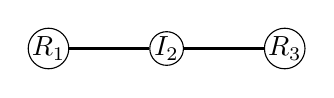
\begin{tikzpicture}[scale=1.5]
    % Draw a 7,11 network
    % First we draw the vertices
    \foreach \pos/\name in {{(1,0)/R_1}, {(2,0)/I_2}, {(3,0)/R_3}}
        \node[vertex] (\name) at \pos {$\name$};
    % Connect vertices with edges 
    \foreach \source/ \dest in {R_1/I_2, I_2/R_3}
        \path[edge] (\source) -- (\dest) ;
        
\end{tikzpicture}
%\end{minipage}
%}
\end{center}

\caption{The state and the network in which the APEX equilibrium does not exist when $k=2$.}
\label{fig:strong_connectedness}
\end{figure}

\begin{example}\label{ex_strong_connectedness}
Suppose $k=2$ and $\theta=(R,I,R)$. The state and the network is represented in Figure~\ref{fig:strong_connectedness}. Rebel 1 never learns the type of player 3 since Inert 2 cannot reveal it, and hence no APEX equilibrium exists in this scenario.
\end{example}

The following assumption on the prior---\textit{full support on strong connectedness}---excludes the possibility of nonexistence of APEX equilibrium. To this end, I begin with the definition of \textit{strong connectedness}.

\begin{definition}[Strong connectedness]
\label{def:strong_connectedness}
Given $G$, a state $\theta$ has strong connectedness if, for every two Rebels, there is a path consisting of Rebels to connect them.

\end{definition}  

In the language of graph theory, the following definition is equivalent: given $G$, $\theta$ has strong connectedness if the induced graph by $[R](\theta)$ is connected.

\begin{definition}[Full support on strong connectedness]\footnote{The prior has full support on strong connectedness is stronger than every state has strong connectedness is common knowledge. This marginal requirement is convenient in constructing equilibrium. The main result only requires a weaker version---$\pi(\theta)>0\Rightarrow \text{ $\theta$ has strong connectedness }$. Working on this weaker version is at the expense of much tedious proof, however.}
Given $G$, $\pi$ has full support on strong connectedness if 
\[\pi(\theta)>0\Leftrightarrow \text{ $\theta$ has strong connectedness}.\]
\end{definition}  

I state the main characterization of this paper:
\begin{theorem}[APEX equilibrium for the case of $1<k<n$]
\label{thm_main_result}
For any $n$-person repeated $k$-Threshold game with parameter $1<k<n$ played in networks, if networks are acyclic and if $\pi$ has full support on strong connectedness, then there is a $\delta^{*}\in(0,1)$ such that an APEX equilibrium exists whenever $\delta>\delta^{*}$.\footnote{A network is acyclic if the path from $i$ to $j$ for all $i\neq j$ is unique.}

\end{theorem}

Constructing an APEX equilibrium in this case is convoluted. I illustrate the proof idea throughout this paper while leaving the formal proof in Appendix. Moreover, since the case of $k=2$ is trivial given that $\theta$ has strong connectedness, I focus on $2<k<n$ cases.\footnote{Suppose $[R](\theta)\geq k=2$, by the full support on strong connectedness, each Rebel have a Rebel neighbor. The following strategy is an APEX strategy. A Rebel plays \textbf{revolt} from period one afterwards if he has a Rebel neighbor; otherwise, he plays \textbf{stay} forever from period one. It extends to an APEX equilibrium by letting the off-path belief be assigning probability one to the event that all non-neighbors are Inerts.} 

I start with considering a specific APEX strategy as the framework in constructing an APEX equilibrium in Section~\ref{sec:apex_strategy}; incentive compatibility is not incorporated at this moment. Then I introduce an auxiliary scenario to illuminate the discussion of incentive compatibility in Section~\ref{sec:writing}. I then go back to present essential details of the constructed APEX equilibrium in Section~\ref{sec:dis_writing}. 

\subsection{APEX strategy}
\label{sec:apex_strategy}
To begin, the following example is examined.
\begin{example}
\label{ex:leading}
Let $k=5$ and consider the configurations in Figure~\ref{fig:circle_with_bridge_5} and Figure~\ref{fig:circle_with_bridge_4}. Note that there are 6 players in both of these configurations; 5 Rebels are in Figure~\ref{fig:circle_with_bridge_5} and 4 Rebels are in Figure~\ref{fig:circle_with_bridge_4}. The below is an APEX strategy.
\[\textbf{Strategy for Example~\ref{ex:leading}:}\]
\begin{enumerate}
\item At period $j$, $1\leq j \leq 6$, each Rebel plays \textbf{revolt} if himself is $j$ or any of his Rebel neighbors is $j$; otherwise, he plays \textbf{stay}. 
For instance, from period one to period 6, what Rebel 3 plays is $(\textbf{revolt},\textbf{stay},\textbf{revolt}, \textbf{revolt},\textbf{stay}, \textbf{revolt})$ in the configuration in Figure~\ref{fig:circle_with_bridge_5}. Consequently, implied by Rebel 3's actions, in the configuration in Figure~\ref{fig:circle_with_bridge_5}, right after period 1, 2, 3, or 4, Rebel 4 is still aware the existence of Rebel 1, 2, 3, and 4; right after period 5, Rebel 4 is aware that player 5 is an Inert; right after period 6, Rebel 4 is aware that player 6 is a Rebel. Similar behavior applies to other players. 
\item Right after period 6, at period 7, by observing his neighbors' actions, a Rebel who has learnt the number of Rebels exceeding or equal to $k$ plays $(\textbf{revolt},\textbf{revolt})$ consecutively. Then he plays \textbf{revolt} from period 19 afterwards. Likewise, a Rebel who has observed the number of Rebels, which is implied by his neighbors' actions, is less than $k$, he plays $(\textbf{stay},\textbf{stay})$ consecutively. Then he plays \textbf{revolt} from period 19 afterwards. A Rebel whose observation does not belong to the above two categories plays the sequence $(\textbf{revolt},\textbf{stay})$ consecutively and plays \textbf{stay} forever after period 19. 
\item From period 7 to period $19$, a Rebel plays $(\textbf{revolt},\textbf{revolt})$ consecutively right after observing the same sequence played by any of his neighbor; he then plays \textbf{revolt} from period 19 afterwards. Correspondingly, a Rebel plays $(\textbf{stay},\textbf{stay})$ consecutively right after observing the same sequence played by any of his neighbor and then plays $\textbf{stay}$ from period 19 afterwards. 
\item The off-path strategy is simple: ignoring the deviation and following the on-path strategy in which more Rebels can be implied. 
\end{enumerate}

By following the on-path strategy of the above, both Rebel 1 and 4 learn the relevant information right after period 7, and all Rebels play the ex-post outcome from period 19 afterwards. This strategy is thus an APEX strategy with a straightforward idea: from period one to period 6, ``a {reporting phase}'', Rebels reports who their Rebel neighbors are by sequences of actions, and, from period 7 to period 19, ``a {coordination phase}'', they coordinate themselves to disseminate the knowledge whether the relevant information is learnt. 
\end{example}

The above strategy, nevertheless, calls for revising to seemly integrate incentive compatibility. Notice that Rebel 6's actions are redundant: the ex-post efficient outcome will be achieved anyway despite how Rebel 6 plays. This is because Rebel 3's neighbors include Rebel 6's and how Rebel 6 plays cannot be observed by other Rebels outside Rebel 3's neighborhood. The notion ``redundant'' will be replaced by and formally defined as \textit{inactive} later to emphasize that Rebel 6 can actually report nothing. What is more, Rebel 4 has no incentive to report. This is because Rebel 1 reports the identical information to the same Rebels. In other words, the ex-post efficient outcome will be played anyway despite how Rebel 4 plays. Rebel 1's position is exactly the same as Rebel 4's, and thus both of them have no incentive to report. A free-rider problem exists.\footnote{It is worth noting that whether a free-rider problem could happen is not solely determined by whether a network is cyclic. It depends on how an APEX strategy is constructed and exists in the constructed APEX equilibrium for Theorem~\ref{thm_main_result}, in which only acyclic networks are of concern. The formal definition of free-rider problem is in Section~\ref{sec:dis_writing}, and a deeper issue will be discussed in Section~\ref{sec:cyclic}.} 

\begin{figure}
\begin{center}
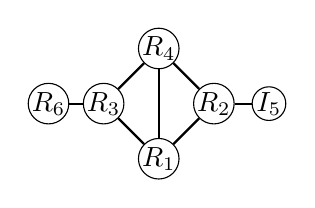
\begin{tikzpicture}[scale=0.7]
    % Draw a 7,11 network
    % First we draw the vertices
    \foreach \pos/\name in {{(2,1)/R_1}, {(3,2)/R_2}, {(1,2)/R_3}, {(2,3)/R_4}, {(4,2)/I_5}, {(0,2)/R_6}}
        \node[vertex] (\name) at \pos {$\name$};
    
%    \foreach \pos/\name in {{(2,3)/I_3}, {(5,3)/I_7}}
%    \node[unknown vertex] (\name) at \pos {$\name$};
    
%    \foreach \pos/\name in {{(3,2)/S_4}, {(4,2)/S_5}}
%    \node[selected vertex] (\name) at \pos {$\name$};
    
    % Connect vertices with edges 
    \foreach \source/ \dest in {R_1/R_4, R_1/R_2, R_1/R_3, R_2/R_4,R_3/R_4, R_2/I_5, R_3/R_6}
        \path[edge] (\source) -- (\dest) ;
        
\end{tikzpicture}
\end{center}
\caption{A configuration of the state and the network in which players 1, 2, 3, 4, 5 are Rebels and players 6 is an Inerts.}
\label{fig:circle_with_bridge_5}
\end{figure}

\begin{figure}
\begin{center}
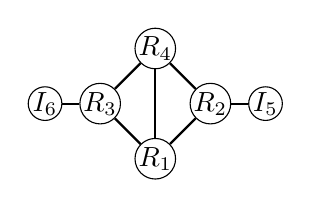
\begin{tikzpicture}[scale=0.7]
    % Draw a 7,11 network
    % First we draw the vertices
    \foreach \pos/\name in {{(2,1)/R_1}, {(3,2)/R_2}, {(1,2)/R_3}, {(2,3)/R_4}, {(4,2)/I_5}, {(0,2)/I_6}}
        \node[vertex] (\name) at \pos {$\name$};
    
%    \foreach \pos/\name in {{(2,3)/I_3}, {(5,3)/I_7}}
%    \node[unknown vertex] (\name) at \pos {$\name$};
    
%    \foreach \pos/\name in {{(3,2)/S_4}, {(4,2)/S_5}}
%    \node[selected vertex] (\name) at \pos {$\name$};
    
    % Connect vertices with edges 
    \foreach \source/ \dest in {R_1/R_4, R_1/R_2, R_1/R_3, R_2/R_4,R_3/R_4, R_2/I_5, R_3/I_6}
        \path[edge] (\source) -- (\dest) ;
        
\end{tikzpicture}
\end{center}
\caption{A configuration of the state and the network in which players 1, 2, 3, 4 are Rebels and player 5, 6 are Inerts.}
\label{fig:circle_with_bridge_4}
\end{figure}

As follows, a revision of Strategy for Example~\ref{ex:leading} is designed and meant to be the foundation framework in constructing the APEX equilibrium for Theorem~\ref{thm_main_result}. Let $\mathbf{I}$ be all possible sets  of Rebels amongst states in the network.\footnote{To be precise, $\mathbf{I}=\{X\subseteq N: \theta_j=R \Leftrightarrow j\in X \text{ for some $\theta\in\Theta$}\}$} 
For convenience, construct a set $W$ that consists of sequences of actions, in which all sequences have equal length, so that there is a one-to-one mapping between $\mathbf{I}$ and $W$. This $W$ exists. For an example, which is used in the constructed APEX equilibrium for Theorem~\ref{thm_main_result}, let the length of each sequence in $W$ be the multiplication of a series of prime numbers. In this series, each prime number is distinct and assigned to a distinct player. Denote $x_i$ as the prime number assigned to $i$. The length of a sequence in $W$ is therefore $\bigotimes_{j\in N}x_j=x_1\otimes...\otimes x_n$, where $\otimes$ is the usual multiplication operator. If $I\in\mathbf{I}$, the corresponding $\langle I \rangle\in W$ is crafted to be:  
\[(\overbrace{\textbf{stay},...,\textbf{stay},\underbrace{\textbf{revolt},\textbf{stay},...,\textbf{stay}}_{\bigotimes_{j\in I}x_j}}^{\bigotimes_{j\in N} x_j}).\]
A one-to-one mapping between $\mathbf{I}$ and ${W}$ exists since a multiplication of prime numbers can be uniquely factorized. 

Fix $W$ and partition the time into two consecutively alternating phases: \textit{coordination phase} and \textit{reporting phase}, while the time is starting from the coordination phase. The $t$-th completion of two consecutive phases is called the $t$-block. The length of each reporting phase is equal to the length of $w\in W$, and the length of each coordination phase is twice of the total number of players. Figure~\ref{fig:ordered_original_game_intro} depicts this partition.\footnote{More precisely, partition the time by $\{\{0\},\{1,...,s_{l_1},s_{l_1}+1,...s_1\},\{s_1+1,...,s_{l_2},s_{l_2}+1,...,s_2\},...,\{s_{t-1}+1,...,s_{l_{t}},s_{l_t}+1,...,s_t\},...\}$, where $t=1,2,...$ and $s_{0}=0$, so that the length of $\{s_{l_t}+1,...,s_t\}$ is equal to the length of $w\in W$ for each $t$, while the length of $\{s_{t-1}+1,...,s_{l_t}\}$ is $2n$. Call $\{s_{t-1}+1,...,s_t\}$ the $t$-block. call $\{s_{l_t}+1,...,s_t\}$ the \textit{reporting phase} at $t$-block and call $\{s_{t-1}+1,...,s_{l_t}\}$ the \textit{coordination phase} at $t$-block.}

\begin{figure}
\[0<\underbrace{(\text{coordination phase})<(\text{reporting phase})}_{\text{$1$-block}}<\underbrace{(\text{coordination phase})<(\text{reporting phase})}_{\text{$2$-block}}<...\]
\caption{The partition of the time in the repeated $k$-threshold game. $<$ is the linear order relation over the time.}
\label{fig:ordered_original_game_intro}
\end{figure}

Given $\theta$, denote the set $I_i$ as $i$'s Rebel neighbors. If $i$ is a Rebel, let $I^1_i= I_i$, and let $I^t_i= \bigcup_{j\in G_i} I^{t-1}_j$ for $t\geq 2$. If $j$ is an Inert, let $I^t_j=\emptyset$ for $t\geq 1$. Put it differently, $I^t_i$ is the set of Rebels who can be reached from Rebel $i$ by a path consisting of Rebels and of which the length is at most $t$. Let us then identify a set of Rebels, \textit{active Rebels}, who are crucial in the information sharing process. For this purpose, first define $G^t_i$ for each $t$: if $i$ is a Rebel, let $G^1_i= G_i$, and let $G^t_i= \bigcup_{j\in G_i} G^{t-1}_j$ for $t\geq 2$; if $j$ is an Inert, let $G^t_j=\emptyset$ for $t\geq 1$. That is, $G^t_i$ is the set of players who can be reached from Rebel $i$ by a path consisting of Rebels and of which the length is at most $t$. Finally, define the active Rebels at $t$-block as follows.
\begin{definition}[Active Rebel at $t$-block]
Set $R^0=[R](\theta)$. The set of active Rebels in the $t$-block is 
\[\text{$R^t:= \{i\in R^{t-1}: \nexists j\in G_i \text{ such that }I^t_i\subseteq G^t_j\}$}.\]
\end{definition}
Otherwise speaking, an active Rebel in the $t$-block is a Rebel whose information about $\theta$, $I^t_i$, is not a subset of any other Rebel's same information. In the configuration in Figure~\ref{fig:circle_with_bridge_5} for Example~\ref{ex:leading}, the set of Rebels is $\{1,2,3,4,6\}$, the active Rebels in the $1$-block are Rebel 2 and 3, and no Rebel is active in the $t$-block when $t\geq 2$. %Take the configuration in Figure~\ref{fig:T-round-4} as another example, $R^0=\{1,2,3,4\}$, $R^1=\{2,3\}$, and $R^2=R^3=...=\emptyset$. 
Notice that the active Rebels have to be also the active ones in the previous block; they are fewer and fewer as $t$ goes by. Let us call a Rebel \textit{inactive Rebel} if he is not an active Rebel.

%\begin{figure}
%
%\begin{center}
%\begin{tikzpicture}[scale=0.7]
%    % Draw a 7,11 network
%    % First we draw the vertices
%    \foreach \pos/\name in {{(1,2)/R_1}, {(2.5,2)/R_2}, {(4,2)/R_3}, {(5.5,2)/R_4}}
%        \node[vertex] (\name) at \pos {$\name$};
%    
%%    \foreach \pos/\name in {{(2,3)/I_3}, {(5,3)/I_7}}
%%    \node[unknown vertex] (\name) at \pos {$\name$};
%    
%%    \foreach \pos/\name in {{(3,2)/S_4}, {(4,2)/S_5}}
%%    \node[selected vertex] (\name) at \pos {$\name$};
%    
%    % Connect vertices with edges 
%    \foreach \source/ \dest in {R_1/R_2, R_2/R_3, R_3/R_4}
%        \path[edge] (\source) -- (\dest) ;
%        
%\end{tikzpicture}
%\end{center}
%\caption{A configuration of the state and the network in which players 1, 2, 3, 4 are Rebels.}
%\label{fig:T-round-4}
%\end{figure}

It is sufficient to reveal the relevant information by letting only active Rebels share information about $\theta$, given that the network is acyclic and given that $\theta$ has strong connectedness. Theorem~\ref{lemma_empty} articulates this.
\begin{theorem}
\label{lemma_empty}
If the network is acyclic and if the $\theta$ has strong connectedness, then there is a strategy so that there exists an active Rebel in the $t$-block who can learn the relevant information at $t+1$-block.
\end{theorem}
Note that $I^t_i\in \mathbf{I}$. The following strategy is for Theorem~\ref{lemma_empty}.\footnote{Theorem~\ref{lemma_empty} is equivalent to the following statement: if the network is acyclic and if the $\theta$ has strong connectedness, then there exists $t\geq 0$ and $i\in R^t$ so that $I^{t+1}_i=[R](\theta)$.} 
\begin{center}
\textbf{Strategy for Theorem~\ref{lemma_empty}:}
\begin{enumerate}
\item In each reporting phase in the $t$-block, each active Rebel $i$ at $t$-block plays $\langle {I^t_i} \rangle\in W$.
\item At each period in each coordination phase in the $t$-block, all Rebels play \textbf{stay}.
\end{enumerate}
\end{center}
\begin{proof} 
Here, I show the proof that there is $t$ and there exists Rebel $i$ who can learn the relevant information in the $t+1$-block. The proof that $i$ has to be active in the $t$-block is in Appendix.  Following the above strategy, right after $t$-block, Rebel $i$ assigns probability one to the event 
\[\{\theta\in \Theta: \text{$\theta_j=R \Leftrightarrow j\in I^{t+1}_i$}\}\] 
by Bayesian rule. To conclude the proof, it is sufficient is to show there exists a $t$ so that $I^{t+1}_i=[R](\theta)$. By definition, $I^t_i$ is the set of Rebels who can be reached by at most $t$ consecutive edges from Rebel $i$, in each of which the endpoints are Rebels. Since $\theta$ has strong connectedness, there exists a $t_i$ so that $I^{t_i}_i=[R](\theta)$. What follows is $i$ learns $\theta$ at $t_i$.
\end{proof}
\begin{remark}
Theorem~\ref{lemma_empty} is not true if the network is cyclic. Take the configuration in Figure~\ref{fig:circle_with_bridge_5} for Example~\ref{ex:leading} as an example. By following Strategy for Theorem~\ref{lemma_empty}, in the $2$-block, there is no Rebel who learns the relevant information. Then, in the $3$-block, either Rebel 1 or 4 learns the relevant information, but both Rebel 1 and 4 are inactive at $2$-block. Theorem~\ref{lemma_empty} thus captures a free-rider problem in cyclic networks as the above mentioned: Rebel 1 and Rebel 4 are redundant mutually.
\end{remark}






%\begin{lemma}
%\label{lemma_inclusion}
%If the $\theta$ has strong connectedness, then 
%$R^t\subseteq R^{t-1}$ for all $t\geq 1$.
%\end{lemma}



Modifying Strategy for Theorem~\ref{lemma_empty}, Strategy for Proposition~\ref{lemma:small_apex} below is an APEX strategy.
\begin{proposition}
\label{lemma:small_apex}
If the network is acyclic and if the $\theta$ has strong connectedness, then there is an APEX strategy.
\end{proposition}
Consider the following strategy. 
\[\textbf{Strategy for Proposition~\ref{lemma:small_apex}:}\]
\begin{enumerate}
\item Suppose $T^{\theta}$ has arrived, Rebels play the ex-post efficient outcome. 
\item Suppose $T^{\theta}$ has not yet arrived. In the reporting phase, Rebels follow Strategy for Theorem~\ref{lemma_empty}. In the coordination phase, as below, the strategy is a contagion process. 
\begin{enumerate}
\item If a Rebel has been certain that there are $k$ or more Rebels, he plays sequence of actions $(\textbf{stay},\textbf{stay})$ continuously starting right after he was certain that. He plays \textbf{stay} forever after this phase; $T^{\theta}$ arrives right after this phase.
\item If a Rebel has learnt that there are less Rebels than $k$ Rebels, he plays sequence of actions $(\textbf{revolt},\textbf{revolt})$ continuously starting right after he learnt that. He plays \textbf{revolt} forever after this phase; $T^{\theta}$ arrives right after this phase.
\item If a Rebel has observed the sequence of actions $(\textbf{stay},\textbf{stay})$, he plays $(\textbf{stay},\textbf{stay})$ continuously starting right after he observed that and plays \textbf{stay} forever after this phase; $T^{\theta}$ arrives right after this phase.
\item If a Rebel has observed the sequence of actions $(\textbf{revolt},\textbf{revolt})$, he plays $(\textbf{revolt},\textbf{revolt})$ continuously starting right after he observed that and plays \textbf{revolt} forever after this phase; $T^{\theta}$ arrives right after this phase.
\item If a Rebel has not learnt the relevant information, he plays sequence of actions $(\textbf{revolt},\textbf{stay})$ continuously.
\end{enumerate} 
\end{enumerate}



This is a simple extension of Strategy for Example~\ref{ex:leading}. Rebels share information in reporting phase. If a Rebel has learnt the relevant information, he disseminates it to all Rebels contagiously in coordination phase; otherwise, he continues to the next phase---a reporting phase. 

If incentive compatibility is under consideration, this logic, however, brings another free-rider problem. Suppose that there are two Rebels who share information to each other in a reporting phase, and each of them is certain that he will learn the relevant information if the other one shares \textit{truthful} information to him. Because sharing information is done by alternating actions, which incurs expected payoff, they will not truthfully share their information. This is because each of them will choose his most profitable way of sharing information without impeding learning the relevant information provided that the other one share the truthful information. The free-rider problem turns out to be the main challenge in the construction of an APEX equilibrium. The proof solves it by arguing that if the network is acyclic, the free-rider problem only occurs between two Rebel neigbors who \textit{commonly know it}, while this argument does not hold for cyclic network.\footnote{Section~\ref{sec:cyclic} provides an example that the free-rider problem is not commonly known between the Rebels who involve.} 
With the help from this argument, the constructed equilibrium solves the free-rider problem by arbitrarily assigning one of them to be the {free rider}, who can choose his most profitable way in sharing information, while letting the other one share truthful information. 

To make the discussion of incentive compatibility more transparent, I introduce \textit{$T$-round writing game} as an auxiliary scenario. In the $T$-round writing game, $T$ is fixed, players are endowed a writing technology so that they can write to share information about $\theta$ for $T$ rounds. They then play a one-shot $k$-threshold game at round $T+1$. This game is a reduced form of the original game by fixing $T$, so that I can pay attention only to the incentive compatibility in information sharing process and ignore the incentive compatibility in the coordination phase.\footnote{There is another free-rider problem in the coordination phase in Strategy for Theorem~\ref{lemma_empty}: a Rebel who has learnt the relevant information might deviate to play $(\textbf{revolt},\textbf{stay})$ from playing $(\textbf{revolt},\textbf{revolt})$. This strategy will be further modified to incorporate the incentive compatibility in Section~\ref{sec:eq_cd}.} 
This writing technology represent a way of communication by \textit{writing sentences that are composed by letters according to a fixed grammar}. Though this auxiliary game will be soon introduced in the next section, I draw Table~\ref{table:analogue} to shed light on the parallel between it and the original game.

\begin{table}[!htbp]
\caption{The analogue between $T$-round writing game and the repeated $k$-threshold game}
\label{table:analogue}
\begin{center}
\begin{tabular}{cc }
$T$-round writing game & Repeated $k$-threshold game \\
\hline
\hline
A round & A range of periods\\
A sentence & A sequence of actions \\
The length of a sentence in a round & The length of a range of periods\\
A chosen letter in a sentence & A chosen action\\
The cost of writing a sentence & The expected payoff occurring in a sequence of actions\\
The fixed grammar & The equilibrium path\\
\hline
\end{tabular}
\end{center}

\end{table}


\subsection{$T$-round writing game}
\label{sec:writing}
The network, the set of states, and the set of players follow exactly the same definitions defined in Section~\ref{sec:model}. In the $T$-round writing game, each player endows a \textit{writing technology}. A writing technology for player $i$ is a pair of $(W,M_i)$, in which $W=\{{\textbf{r}},\textbf{s}\}^L$, $L\in \mathbb{N}$, and $M:= \bigtimes_{i\in N}\bigtimes^T_{t=1}M^{t}_i$ recursively defined by
\[M^1_i=\{f|f:\Theta_{G_i}\rightarrow W\}\cup \{\emptyset\}\]
\[ \text{ for } 2\leq t \leq T\text{ , }M^{t}_i=\{f|f:\bigtimes_{j\in G_i}M^{t-1}_j\rightarrow W\}\cup \{\emptyset\}. \]
$W$ is interpreted as the set of sentence composed by letters \textbf{r} or \textbf{s} with length $L$, while $M_i$ is understood as $i$'s grammar. $\emptyset$ represents remaining silent. The phrase of ``$i$ writes a sentence to all his neighbors at round $t$'' is equivalent to ``$i$ selects an $f\in M^t_i$ to get an element $w\in W$ according to $f$, which can be observed by all $i$'s neighbors''. 
%A sentence being a mixture of two sentences $w,w^{'}\in W$ is denoted as $w\oplus w^{'}$ with the property that $(w\oplus w^{'})_l=\textbf{r}$ if and only if $w_l=\textbf{r}$ or $w^{'}_l=\textbf{r}$ for all $l\in \{1,...,L\}$. 

The time line for the deterministic $T$-round writing game is as follows.
\begin{enumerate}
\item Nature chooses $\theta$ according to the prior $\pi$.
\item $\theta$ is then fixed throughout rounds.
\item At $t=1,...,T$ round, players write to their neighbors. 
\item At $T+1$ round, players play a one-shot $k$-Threshold game.
\item The game ends.
\end{enumerate}
%\begin{table}[!htbp]
%\begin{center}
%\begin{tabular}{ll }
%1.  & Nature chooses $\theta$ according to $\pi$. \\
%2. & $\theta$ is then fixed throughout rounds.\\
%3. & At $t=1,...,T$ round, players write to their neighbors. \\
%4. & At $T+1$ round, players play a one-shot $k$-Threshold game.\\
%5. & The game ends.
%\end{tabular}
%\end{center}
%\end{table}
A Rebel's payoff is the summation of his stage payoff across stages, while an Inert's payoff is set to be $1$. The equilibrium concept is weak sequential equilibrium. An APEX strategy is a strategy that induces the ex-post outcome in the one-shot $k$-threshold game at $T+1$ round. The definition of APEX equilibrium is adapted accordingly. In the examples below, let us focus on the configuration represented in Figure~\ref{fig:T-round-6} and Figure~\ref{fig:T-round-5} with $n=L=8$. I.e.~there are 8 players and the length of a sentence is also 8. Note that the differences between configurations in Figure~\ref{fig:T-round-6} and Figure~\ref{fig:T-round-5} are: (1) there are 6 Rebels in Figure~\ref{fig:T-round-6} but are 5 Rebels in Figure~\ref{fig:T-round-5}; (2) player 8 is a Rebel in Figure~\ref{fig:T-round-6} but he is an Inert in Figure~\ref{fig:T-round-6}.

\begin{figure}

\begin{center}
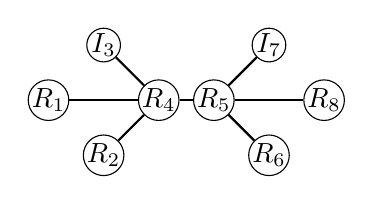
\begin{tikzpicture}[scale=0.7]
    % Draw a 7,11 network
    % First we draw the vertices
    \foreach \pos/\name in {{(1,2)/R_1}, {(2,1)/R_2}, {(5,1)/R_6}, {(6,2)/R_8}, {(3,2)/R_4}, {(4,2)/R_5}}
        \node[vertex] (\name) at \pos {$\name$};
    
    \foreach \pos/\name in {{(2,3)/I_3}, {(5,3)/I_7}}
    \node[unknown vertex] (\name) at \pos {$\name$};
    
%    \foreach \pos/\name in {{(3,2)/S_4}, {(4,2)/S_5}}
%    \node[selected vertex] (\name) at \pos {$\name$};
    
    % Connect vertices with edges 
    \foreach \source/ \dest in {R_1/R_4, R_2/R_4,I_3/R_4,R_4/R_5, R_5/R_6, R_5/I_7, R_5/R_8}
        \path[edge] (\source) -- (\dest) ;
        
\end{tikzpicture}
\end{center}
\caption{A configuration of the state and the network in which players 1, 2, 4, 5, 6, 8 are Rebels while players 3, 7 are Inerts.}
\label{fig:T-round-6}
\end{figure}

\begin{figure}

\begin{center}
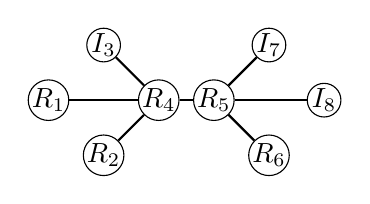
\begin{tikzpicture}[scale=0.7]
    % Draw a 7,11 network
    % First we draw the vertices
    \foreach \pos/\name in {{(1,2)/R_1}, {(2,1)/R_2}, {(5,1)/R_6}, {(3,2)/R_4}, {(4,2)/R_5}}
        \node[vertex] (\name) at \pos {$\name$};
    
    \foreach \pos/\name in {{(2,3)/I_3}, {(5,3)/I_7}, {(6,2)/I_8}}
    \node[unknown vertex] (\name) at \pos {$\name$};
    
%    \foreach \pos/\name in {{(3,2)/S_4}, {(4,2)/S_5}}
%    \node[selected vertex] (\name) at \pos {$\name$};
    
    % Connect vertices with edges 
    \foreach \source/ \dest in {R_1/R_4, R_2/R_4,I_3/R_4,R_4/R_5, R_5/R_6, R_5/I_7, R_5/I_8}
        \path[edge] (\source) -- (\dest) ;
        
\end{tikzpicture}
\end{center}
\caption{A configuration of the state and the network in which players 1, 2, 4, 5, 6 are Rebels while players 3, 7, 8 are Inerts.}
\label{fig:T-round-5}
\end{figure}

%
%\subsubsection{$T$-round writing game with cheap talk}
%\label{sec:cheap_talk}
%\begin{example}[Deterministic $T$-round writing without cost---cheap talk]
%\label{ex:cheap_talk}
%Let $k=6$, $T=2$, and suppose writing is costless. This is, there are two rounds for writing, while writing is the same as cheap talk.
%%Let the grammar for Rebel 4 (or 5) be: \textbf{r} is written in the $i$-th component if player $i$ is a Rebel; \textbf{s} is written in the $j$-th component if $j$'s type is an Inert or unknown to Rebel 4 (or 5).
%
%Consider the following strategy $\phi$. 
%
%At $t=1$, the peripheral Rebels remain silent. Rebel 4 (or 5)'s grammar for writing a sentence is: if player $i$ is a Rebel and known to him, he writes \textbf{r} in the $i$-th component in the sentence; otherwise, he writes \textbf{s} in that component. According to this grammar, the central player Rebel 4 writes the sentence $(\textbf{r},\textbf{r},\textbf{s},\textbf{r},\textbf{r},\textbf{s},\textbf{s},\textbf{s})$ on both configurations in Figure~\ref{fig:T-round-6} and in Figure~\ref{fig:T-round-5}. The central player Rebel 5 writes $(\textbf{s},\textbf{s},\textbf{s},\textbf{r},\textbf{r},\textbf{r},\textbf{s},\textbf{r})$ in the configuration in Figure~\ref{fig:T-round-6} and writes $(\textbf{s},\textbf{s},\textbf{s},\textbf{r},\textbf{r},\textbf{r},\textbf{s},\textbf{s})$ in the configuration in Figure~\ref{fig:T-round-5}.\footnote{The notion of ``peripheral'' and ``central'' will be formalized in Section~\ref{sec:info}} Rebels 4 and 5's sentences thus reveals who are Rebels and who are not. Notice that the common knowledge of the network contributes to the ability of revealing players' types. 
%
%At $t=2$, the peripheral Rebels still remain silent. Rebel 4 writes $(\textbf{r},\textbf{r},\textbf{s},\textbf{r},\textbf{r},\textbf{r},\textbf{s},\textbf{r})$ in the configuration in Figure~\ref{fig:T-round-6} and writes $(\textbf{r},\textbf{r},\textbf{s},\textbf{r},\textbf{r},\textbf{r},\textbf{s},\textbf{s})$ in the configuration in Figure~\ref{fig:T-round-5}. Rebel 5 writes exactly the same sentence as Rebel 4. This is to say Rebel 4 and 5 share information at $t=1$ and then coordinate to announce a mixture sentence at $t=T$. 
%
%At $T+1$, by counting \textbf{r} in Rebel 4 or 5's mixture sentence, all Rebels know whether the number of Rebels outnumbers $k$. This leads all Rebels to play the ex-post efficient outcome in the one-shot $k$-threshold game. 
%
%%Suppose the configuration is that in Figure~\ref{fig:T-round-5}. At $t=1$, similarly, $\phi$ prescribes that Rebels 1,2,6,8 keep silent; Rebel 4 writes $(\textbf{r},\textbf{r},\textbf{s},\textbf{r},\textbf{r},\textbf{s},\textbf{s},\textbf{s})$; Rebel 5 writes $(\textbf{s},\textbf{s},\textbf{s},\textbf{r},\textbf{r},\textbf{r},\textbf{s},\textbf{s})$. At $t=2$, however, $\phi$ prescribes that the peripheral Rebels 1,2,6,8 keep silent; Rebel 4 keeps silent; Rebel 5 keeps silent as well. On the path, keeping silent by Rebel 4 (or 5) reflects that Rebel 4 (or 5) knows that the total number of Rebels is less than $k=6$. At $t=3$, all Rebels know this relevant information and play the ex-post efficient outcome \textbf{stay}.
%
%
%\end{example}
%
%\begin{remark}
%An assessment $(\phi,\omicron)$, where $\omicron$ is a belief system, is made to be an APEX equilibrium for Example~\ref{ex:cheap_talk} above as follows. The off-path strategy of $\phi$ prescribes that if there is a detectable deviation, then the Rebels who detect this deviation will remain silent until $t=T$ and then play \textbf{stay} at $T+1$.\footnote{A deviation could be, for instance, a wrong sentence that is not grammatical, is deviating from the on-path $\phi$,..., etc} 
%The off-path belief of $\omicron$ is to believe that all players who are not neighbors are Inerts. The on-path belief of $\omicron$ is the belief induced by $\phi$. Since any deviation by Rebel 4 or 5 would strictly decrease the possibility of achieving an ex-post efficient outcome, and writing is costless, the assessment $(\phi,\omicron)$ constitutes an APEX equilibrium.
%\end{remark}
%\begin{example}[Deterministic $T$-round writing with a fixed cost]
%\label{ex:fixed_cost_talk}
%Let $k=6$ and $T=2$. Suppose that writing incurs a fixed cost $\epsilon>0$ while keeping silent does not. Let us consider the assessment $(\phi,\omicron)$ in the above example. Since any deviation by Rebel 4 or 5 would strictly decrease the possibility to achieve the ex-post efficient outcome while the ex-post efficient outcome will give the maximum expected payoff for every Rebel at $t=3=T+1$ if the relevant information can be revealed then, if $\epsilon$ is sufficiently small, $(\phi,\omicron)$ also constitutes an APEX equilibrium.
%
%\end{example}

%If writing is costly instead, the next example shows that $(\phi,\omicron)$ is not an APEX equilibrium. This is due to the free-rider problem.

\begin{example}[$T$-round writing and the free-rider problem]
\label{ex:cost_function_talk_fr}
Let $k=6$ and $T=2$. Suppose that remaining silent incurs no cost, but writing incurs an extremely small cost $\epsilon>0$ so that $\epsilon$ is strictly decreasing with the number of \textbf{r} in a sentence. This is to say writing $(\textbf{r},\textbf{r},\textbf{r},\textbf{r},\textbf{r},\textbf{r},\textbf{r},\textbf{r})$ incurs the least cost while writing $(\textbf{s},\textbf{s},\textbf{s},\textbf{s},\textbf{s},\textbf{s},\textbf{s},\textbf{s})$ incurs the largest.\footnote{This cost is not directly linking to the expected payoff in the original game, but is meant to be a metaphor to emphasize that alternating actions might incurs negative expected payoff in the original game and to illustrate the potential free-rider problem.} 

Let us consider the following strategy $\phi$. 

At $t=1$, the peripheral Rebels remain silent. Rebel 4 (or 5)'s grammar for writing a sentence is that if player $i$ is a Rebel and known to him, he writes \textbf{r} in the $i$-th component in the sentence; otherwise, he writes \textbf{s} in that component. According to this grammar, the central player Rebel 4 writes the sentence $(\textbf{r},\textbf{r},\textbf{s},\textbf{r},\textbf{r},\textbf{s},\textbf{s},\textbf{s})$ on both configurations in Figure~\ref{fig:T-round-6} and in Figure~\ref{fig:T-round-5}. The central player Rebel 5 writes $(\textbf{s},\textbf{s},\textbf{s},\textbf{r},\textbf{r},\textbf{r},\textbf{s},\textbf{r})$ in the configuration in Figure~\ref{fig:T-round-6} and writes $(\textbf{s},\textbf{s},\textbf{s},\textbf{r},\textbf{r},\textbf{r},\textbf{s},\textbf{s})$ in the configuration in Figure~\ref{fig:T-round-5}. Rebels 4 and 5's sentences thus reveals who are Rebels and who are not. Notice that the common knowledge of the network contributes to the ability of revealing players' types. 

At $t=2$, the peripheral Rebels still remain silent. Rebel 4 writes $(\textbf{r},\textbf{r},\textbf{s},\textbf{r},\textbf{r},\textbf{r},\textbf{s},\textbf{r})$ in the configuration in Figure~\ref{fig:T-round-6} and writes $(\textbf{r},\textbf{r},\textbf{s},\textbf{r},\textbf{r},\textbf{r},\textbf{s},\textbf{s})$ in the configuration in Figure~\ref{fig:T-round-5}. Rebel 5 writes exactly the same sentence as Rebel 4. This is to say Rebel 4 and 5 share information at $t=1$ and then coordinate to announce a mixture sentence at $t=T$. 

At $T+1$, by counting \textbf{r} in Rebel 4 or 5's mixture sentence, all Rebels know whether the number of Rebels outnumbers $k$. This leads all Rebels to play the ex-post efficient outcome in the one-shot $k$-threshold game. 

The above $\phi$ is not an APEX equilibrium. According to the above-mentioned, Rebel 4 will know the relevant information at $t=2$ even if he deviates to writing that all his neighbors are Rebels, which incurs less cost than his truthful writing.\footnote{This sentence is $(\textbf{r},\textbf{r},\textbf{r},\textbf{r},\textbf{r},\textbf{s},\textbf{s},\textbf{s})$, which incurs less cost than the truthfully reporting sentence $(\textbf{r},\textbf{r},\textbf{s},\textbf{r},\textbf{r},\textbf{s},\textbf{s},\textbf{s})$.}\footnote{If he remains silent, then this behavior will be considered as a deviation, and therefore he will never get the maximum payoff of $1$. Hence, he will avoid doing so.}
Rebel 5 is in the same situation as Rebel 4 and therefore also writes the sentence that indicates that all his neighbors are Rebels. However, these sentences are uninformative. It turns out that both of them will deviate, and neither of them can know the relevant information at $t=2$.
%\footnote{Actually, one can claim there is no APEX equilibrium in this case by contraposition. If there is one, say $(\phi^{'},\omicron^{'})$, then on the path of $\phi^{'}$, some Rebels should write and play differently in different configurations. Suppose Rebel 5 will play differently to truthfully reveal his information at $t=1$. Rebel 4 has two kinds of strategies then. He might write the least-cost sentence or he could write something depending on his information. For the former case, since Rebel 4 will be the only one who know the relevant information, he should write to Rebel 5 to let Rebel 5 pass this information to the remaining Rebels. However, it requires two rounds to pass it, but there is only one round left. For the latter case, if Rebel 4 truthfully reveal his information, the Rebel 5 will deviate to writing least-cost sentence; if Rebel 4's information is not truthfully reveal, there is a prior so that the ex-post outcome will not be played.}


\end{example}

Fortunately, the following example shows that the free-rider problem can be solved. 

\begin{example}[$T$-round writing and solving the free-rider problem]
\label{ex:cost_function_talk_solve_fr}
The solution to solve the free-rider problem in the previous example is to extend $T$. It would open the possibility of the existence of a free rider at some round, while letting this free rider reveals relevant information at the next round. To this end, let $k=6$ and $T=3$. Consider the following strategy $\rho$ and focus on the interaction between Rebels 4 and 5.
%First note that if the previous strategy $\phi$ is extended to the current case so that Rebel 4 and 5 still simultaneously truthfully write their information at either $t=1$ or $t=2$, $\phi$ is not an equilibrium path by the same free-rider argument as the above. 

At $t=1$, the lowest-index Rebel between Rebels 4 and 5 is the free rider, while the other one truthfully writes down his information. This is to say Rebel 4 will be the free rider and he writes the least-cost sentence. Rebel 5 writes $(\textbf{s},\textbf{s},\textbf{s},\textbf{r},\textbf{r},\textbf{r},\textbf{s},\textbf{r})$ in the configuration of Figure~\ref{fig:T-round-6}and writes $(\textbf{s},\textbf{s},\textbf{s},\textbf{r},\textbf{r},\textbf{r},\textbf{s},\textbf{s})$ in the configuration of Figure~\ref{fig:T-round-5}. 

At $t=2$, Rebel 4 has known the relevant information. Rebel 4 writes the least-cost sentence if there are $k$ or more Rebels but remains silent otherwise. The consequence is Rebel 4's behavior reveals the relevant information to his neighbors at this round. Rebel 5 remains silent instead. 

At $t=T$, Rebel 5 has known the relevant information since he is Rebele 4's neighbor. He writes the least-cost sentence if there are $k$ or more Rebels but remains silent otherwise. Therefore Rebel 5's behavior at this round reveals the relevant information to his neighbors. Rebel 4 remains silent instead.

At $T+1$, all Rebels know the relevant information by observing Rebels 4 and 5's behavior. They play the ex-post efficient outcome accordingly. 
%To construct an APEX equilibrium from $\rho$, recall $(\phi,\omicron)$ and let the on-path belief of $\dot{\omicron}$ be induced by $\rho$. The off-path strategy follows that in $\phi$, and the off-path belief follows that of $\omicron$.   



\end{example}

\begin{remark}
Why does Rebel 5 \textit{know} that he is not a free rider and therefore behaves not like a free rider? The following is the reason. He \textit{knows} that, by common knowledge of the network, he and Rebel 4 are in a free-rider problem. Moreover, by common knowledge of the network, he knows that Rebel 4 knows that he and Rebel 4 are in a free-rider problem, he knows that Rebels 4 knows that he knows that,...,and so forth. Consequently, Rebel 5 and 4 commonly know that they are engaged in a free-rider problem. 
\end{remark}
In the next section, Section~\ref{sec:dis_writing}, I delver into substantial ideas in constructing an APEX equilibrium and leave actual details in Appendix. Separately, I depict the construction in the reporting phase and in the coordination phase. The depiction might seem repetitive, but deliberately tailored. Especially, so far, the attention is devoutly paid to integrating incentive compatibility in the reporting phase, but in the lack of the coordination phase. Section~\ref{sec:eq_cd} manages the incentive compatibility in the coordination phase.
\subsection{Equilibrium construction}
\label{sec:dis_writing}
The framework is adapted from Proposition~\ref{lemma:small_apex}, and the time is partitioned by two consecutively alternating phases as shown in Figure~\ref{fig:ordered_original_game_intro}. Recall that the time is partitioned into
\[0<\underbrace{(\text{coordination phase})<(\text{reporting phase})}_{\text{$1$-block}}<\underbrace{(\text{coordination phase})<(\text{reporting phase})}_{\text{$2$-block}}<...\]

The off-path belief is simple and serves as a grim trigger. Whenever Rebel $i$ detects a deviation at period $\varsigma$, he forms the following belief: 
\begin{equation}
\label{eq_grim_trigger}
\sum_{\theta \in \{\theta:\theta_j=I,j\notin G_i\}}\beta^{\pi,\tau}_{G_i}({\theta}|h^{s}_{G_i})=1 \text{, for all $s\geq \varsigma$}.
\end{equation}
This is to say $i$ believe all players outside his neighborhood are Inerts. Thus, if $\# I^{\varsigma}_i<k$, he will play \textbf{stay} forever after he detects a deviation. 

\subsubsection{The equilibrium path in the reporting phase}
\label{sec:eq_rp}
The description in this section is for the APEX equilibrium path {before} $T^{\theta}$. Let us shorten ``reporting phase in $t$-block'' by $\Omicron^{t}$, denote $|\Omicron^t|$ as the length of $\Omicron^{t}$, and shorten \textbf{revolt} and \textbf{stay} to \textbf{r} and \textbf{s} receptively. For simplicity, the term ``reporting phase'' refers to ``reporting phase in $t$-block'' in this section.

$|\Omicron^{t}|$ is independent from $t$ and determined only by the set of players. Firstly, assign each player $i$ a distinct prime number $x_i$ starting from $3$. Then let $|\Omicron^{t}|=\bigotimes_{i\in N} x_i=x_1\otimes x_2\otimes...\otimes x_n$ , where $\otimes$ is the usual multiplication operator. The sequence of actions in $\Omicron^{t}$ is with length $|\Omicron^t|$ and would take one of the forms specified in the right column in Table~\ref{Table_msg_form}. The abbreviations of these sequences are listed in the left column. Since these sequences in the reporting phase are meant to share information about $\theta$, the terms ``playing the sequence'' and ``reporting the information'' are interchangeable and will be alternatively used.


\begin{table}[!htbp]
\caption{The notations for the sequences of actions in $\Omicron^t$ on the path}
\label{Table_msg_form}
\begin{center}
\begin{tabular}{l c c}
Notations && The sequences of actions\\
\hline
\hline
$\langle  I \rangle$ 				& $:=$ 			& $(\overbrace{\textbf{s},...,\textbf{s},\underbrace{\textbf{r},\textbf{s},...,\textbf{s}}_{\bigotimes_{j\in I}x_j} }^{\bigotimes_{i\in N} x_i})$  \\
$\langle 1 \rangle$	 					& $:=$ 			& $( \overbrace{\textbf{s},...,\textbf{s},{\textbf{r}} }^{\bigotimes_{i\in N} x_i} )$  \\
$\langle \textbf{all stay} \rangle$	 					& $:=$ 			& $(\overbrace{ \textbf{s},...,\textbf{s},{\textbf{s}} }^{\bigotimes_{i\in N} x_i})$  \\
\hline
\end{tabular}
\end{center}
\end{table}


It is worth noting that the sequence constructed by prime numbers brings two benefits. Firstly, since the multiplication of distinguishing prime numbers can be uniquely factorized, the Rebels can use such sequence to precisely report players' identities. Secondly, the un-discounted expected payoff of playing $\langle I^t_i \rangle$ for some $I^t_i$ for an active Rebel $i$ is always equal to $-1$, and therefore it is relatively easy to calculate. This is because only active Rebels will report $\langle I \rangle$ for some $I$. Since this $I$ is not reported by any other Rebel, at most one Rebel would play \textbf{r} at any period in the reporting phase by the property of prime number multiplication.\footnote{This statement holds if there is no Rebel who plays $\langle 1 \rangle$.} 

I list the sequences played in the reporting phase on the path in Table~\ref{Table_msg_RP_path}. The terms $\theta$-pivotal, $k-1$-pivotal, and free-rider problem will be defined one-paragraph later.

\begin{table}[!htbp]
\caption{The sequences of actions played in $\Omicron^t$ on the path}
\label{Table_msg_RP_path}
\begin{center}
\begin{tabular}{l c}
Rebel $i$ & $i$ plays\\
\hline
\hline
$i$ is inactive				& $\langle \textbf{all stay} \rangle$  \\
$i$ is active but $i$ is not pivotal	 					 			& $\langle I^t_i \rangle$  \\
$i$ is $k-1$-pivotal	 					 			& $\langle 1 \rangle$  \\
$i$ is $\theta$-pivotal but not in the free-rider problem	 					 			& $\langle 1 \rangle$  \\
$i$ is in the free-rider problem with the lowest index	 					 			& $\langle 1 \rangle$  \\
$i$ is in the free-rider problem without the lowest index	 					 			& $\langle I^t_i \rangle$  \\
\hline
\end{tabular}
\end{center}
\end{table}

On the path, the sequences $\langle I \rangle$ or $\langle 1 \rangle$ are meant to differentiate themselves from $\langle \textbf{all stay} \rangle$. The sequence $\langle \textbf{all stay} \rangle$ is for the inactive Rebels at $t$-block to report nothing. The sequence $\langle I \rangle$ is for active Rebels at $t$-block to report $I$ if $I$ is a set of Rebels. Although the definitions of \textit{pivotal Rebel} and \textit{free-rider problem} has not yet formally defined at this present, the sequence $\langle 1 \rangle$ is intentionally crafted to tackle the free-rider problem. To see how $\langle 1 \rangle$ works, I turn to formally defining the {pivotal Rebel} and the {free-rider problem}. 

\begin{definition}[Pivotal Rebels in $\Omicron^t$]
A Rebel $p$ is pivotal in $\Omicron^t$ if $p$ is uncertain the relevant information at $t$-block, and $p$ is certain that he will learn the relevant information right after $\Omicron^t$, given that each $i\in R^t$ reports $\langle I^t_i \rangle$.
\end{definition}

By the definition, a pivotal Rebel in the reporting phase is one who can learn the relevant information if all of his active Rebel neighbors truthfully report their information about $\theta$ to him. The pivotal Rebels can be further classified into two kinds: ones who can learn $\theta$, and ones who learn only the relevant information. When $k=6$, in the configuration in Figure~\ref{fig:T-round-6}, only Rebels 4 and 5 are pivotal; they are of the first kind. In the configuration in Figure~\ref{fig:central_pivotal}, only Rebel 5 is pivotal; he is of the first kind. In the configuration in Figure~\ref{fig:k-1_pivotal}, only Rebel 4 pivotal; he is of the second kind.

%\begin{figure}
%
%\begin{center}
%\begin{tikzpicture}[scale=0.7]
%    % Draw a 7,11 network
%    % First we draw the vertices
%    \foreach \pos/\name in {{(1,2)/R_1}, {(2,1)/R_2}, {(5,1)/R_6}, {(6,2)/R_8}, {(3,2)/R_4}, {(4,2)/R_5}}
%        \node[vertex] (\name) at \pos {$\name$};
%    
%    \foreach \pos/\name in {{(2,3)/I_3}, {(5,3)/I_7}}
%    \node[unknown vertex] (\name) at \pos {$\name$};
%    
%%    \foreach \pos/\name in {{(3,2)/S_4}, {(4,2)/S_5}}
%%    \node[selected vertex] (\name) at \pos {$\name$};
%    
%    % Connect vertices with edges 
%    \foreach \source/ \dest in {R_1/R_4, R_2/R_4,I_3/R_4,R_4/R_5, R_5/R_6, R_5/I_7, R_5/R_8}
%        \path[edge] (\source) -- (\dest) ;
%        
%\end{tikzpicture}
%\end{center}
%\caption{A configuration of the state and the network in which players 1, 2, 4, 5, 6, 8 are Rebels while players 3, 7 are Inerts.}
%\label{fig:T-round-6}
%\end{figure}


\begin{figure}

\begin{center}
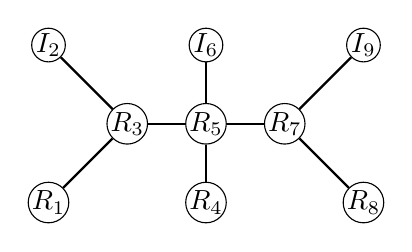
\begin{tikzpicture}[scale=1]
    % Draw a 7,11 network
    % First we draw the vertices
    \foreach \pos/\name in {{(1,1)/R_1}, {(1,3)/I_2}, {(2,2)/R_3}, {(3,1)/R_4}, {(3,2)/R_5}, {(3,3)/I_6}, {(4,2)/R_7}, {(5,1)/R_8}, {(5,3)/I_9}}
        \node[vertex] (\name) at \pos {$\name$};
    
    
    % Connect vertices with edges 
    \foreach \source/ \dest in {R_1/R_3, I_2/R_3, R_3/R_5, R_4/R_5, I_6/R_5, R_5/R_7, R_7/R_8, R_7/I_9}
        \path[edge] (\source) -- (\dest) ;
        
\end{tikzpicture}
\end{center}
\caption{A configuration of the state and the network in which player 1, 3, 4, 5, 7, 8 are Rebels while players 2, 4, 9 are Inerts.}
\label{fig:central_pivotal}
\end{figure}

\begin{figure}


\begin{center}
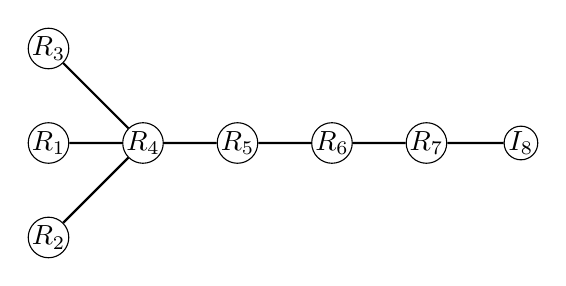
\begin{tikzpicture}[scale=1.2]
    % Draw a 7,11 network
    % First we draw the vertices
    \foreach \pos/\name in {{(2,2)/R_1}, {(2,1)/R_2}, {(2,3)/R_3}, {(3,2)/R_4}, {(4,2)/R_5}, {(5,2)/R_6}, {(6,2)/R_7}, {(7,2)/I_8}}
        \node[vertex] (\name) at \pos {$\name$};
    
    
    % Connect vertices with edges 
    \foreach \source/ \dest in {R_1/R_4, R_2/R_4,R_3/R_4,R_4/R_5, R_5/R_6, R_6/R_7, R_7/I_8}
        \path[edge] (\source) -- (\dest) ;
        
\end{tikzpicture}
\end{center}
\caption{A configuration of the state and the network in which player 1, 2, 3, 4, 5, 6, 7 are Rebels while player 8 is an Inert.}
\label{fig:k-1_pivotal}
\end{figure}

Call $p$ of the first kind the \textit{$\theta$-pivotal} Rebel. For the second kind, if the network is acyclic and if the prior has full support on strong connectedness, $p$ is the second kind only if $I^{t}_p=k-1$. Call this second kind \textit{$k-1$-pivotal} Rebel.\footnote{To show that a pivotal Rebel is the second kind in $\Omicron^{t}$ only if $I^{t}_p=k-1$, one can follow the same argument in Theorem~\ref{lemma_empty}.} Below is the defined free-rider problem in the reporting phase.

\begin{definition}
A free-rider problem exists in $\Omicron^t$ if there are multiple $\theta$-pivotal Rebels in $\Omicron^t$.
\end{definition}



The following lemma is crucial. 
%it says that there will be at most two $\theta$-pivotal Rebels in $R^{t}$. Therefore, if there is a free-rider problem, it occurs between two $\theta$-pivotal Rebels. Moreover, if there are two of them, they are neighbors. (... it occurs between two Rebels who are neighbors.)
\begin{lemma}
\label{lemma_at_most_two_nodes}
If the network is acyclic and if $\pi$ has full support on strong connectedness, there are at most two active $\theta$-pivotal Rebels in the $t$-block. Moreover, they are neighbors.\footnote{As a remark, Lemma~\ref{lemma_at_most_two_nodes} is not true when the network is cyclic. To see this, consider a 4-player circle given that $\theta=(R,R,R,R)$.}
\end{lemma}

And notably,

\begin{lemma}
\label{lemman_pivotals_CK}
If the network is acyclic and if $\pi$ has full support on strong connectedness, when there are two active $\theta$-pivotal Rebels $p,p^{'}$ in the $t$-block, then they commonly know that they are $\theta$-pivotal Rebels at the beginning of $t$-block.
\end{lemma}

By Lemma~\ref{lemman_pivotals_CK}, $\theta$-pivotal Rebels in the reporting phase can identify themselves at the beginning of this phase. This importance cannot be further emphasized. If the free-rider problem will occurs in the reporting phase, the strategy can, before the reporting phase, prescribes that the lowest indexed $\theta$-pivotal Rebel $p$ involving in the free-rider problem will play $\langle 1 \rangle$, while the other one will play $\langle I^t_{p^{'}} \rangle$. Otherwise speaking, this knowledge is encoded in the belief system of an APEX equilibrium. 

\begin{remark}
As the above mentioned, the assumption of acyclic network in Lemma~\ref{lemman_pivotals_CK} is indispensable. Lemma~\ref{lemman_pivotals_CK} does not hold if the network is cyclic. Section~\ref{sec:cyclic} demonstrates it.
\end{remark}






\subsubsection{The equilibrium path in the coordination phase}
\label{sec:eq_cd}
The descriptions in this section is for the APEX equilibrium path {before} $T^{\theta}$. The term ``coordination phase in $t$-block'' is shorten by $\Kappa^{t}$.  

It is elaborate to spell out the coordination phase structure, but this phase is actually a simple contagion scenario: Rebels jointly decide to terminate or continue their information sharing during this phase. For that, a coordination phase is partitioned into three \textit{divisions}. In the first division, if there is a Rebel has learnt that $\#[R](\theta)<k$, all Rebels will play \textbf{stay} forever right after this division, and $T^{\theta}$ arrives; otherwise, they continue to the next one. In the second division, if there is a Rebel has learnt that $\#[R](\theta)\geq k$, a portion of Rebels, at least $k$ Rebels, will play \textbf{revolt} forever right after this division; otherwise, they continue to the next one. In the third division, if there is a Rebel has learnt that $\#[R](\theta)\geq k$ in the previous divisions, all Rebel will play \textbf{revolt} forever right after this division, and $T^{\theta}$ arrives; otherwise, they continue to the next phase---a reporting phase.

To fulfil the above contagion argument, a set of sequences of actions played on the path is prescribed so that Rebels update their belief according to it. For this task, further partition a division into \textit{sub-blocks}. I depict the whole partition in the coordination phase below, where $\Box$ represents a sub-block in a coordination phase. 

In $\Kappa^1$, 
\[\overbrace{\underbrace{ \Box }_{\text{one sub-block}}}^{\text{$1$-division}} \overbrace{\underbrace{\Box }_{\text{one sub-block}}}^{\text{$2$-division}} \overbrace{\underbrace{\Box \cdot \cdot \cdot \Box}_{\text{$n$ sub-blocks}}}^{\text{$3$-division}}\] 

In $\Kappa^t$, $t\geq 2$,
\[\overbrace{\underbrace{\Box \cdot \cdot \cdot \Box}_{\text{$n$ sub-blocks}}}^{\text{$1$-division}} \overbrace{\underbrace{\Box \cdot \cdot \cdot \Box}_{\text{$t+1$ sub-blocks}} }^{\text{$2$-division}} \overbrace{\underbrace{\Box \cdot \cdot \cdot \Box}_{\text{$n$ sub-blocks}}}^{\text{$3$-division}}\] 




For each $t$, denote $\Kappa^t(u,\cdot)$ as the $u$-division and $|\Kappa^t(u,\cdot) |$ as the length of $\Kappa^t(u,\cdot)$. Likewise, denote $\Kappa^t(u,v)$ as the $v$-th sub-block in $u$-division and $|\Kappa^t(u,v) |$ as the length of $\Kappa^t(u,v)$. Let us shorten \textbf{revolt} and \textbf{stay} to \textbf{r} and \textbf{s} receptively. 

Let
\[
    |\Kappa^t(u,v)|=\left\{
                \begin{array}{lcl}
                  n & \text{if} & u=1,2, v=1,...,n.\\
                 1 & \text{if} & u=3, v=1,...,n.
                \end{array}
              \right. 
\]


Let $|\Kappa^t(u,v)|=n$ if $u=1,2$, $v=1,...,n$. Let $|\Kappa^t(u,v)|=1$ if $u=3$, $v=1,...,n$. I list the the sequences of actions on the path and their notations in Table~\ref{Table_msg_coordination}, where $i$ is the original index of player $i$.
%\footnote{In the $3$-division, since the sequence of actions which length is 1 is equivalent to playing a single action, I do not provide additional notations for conciseness.}



\begin{table}[!htbp]
\caption{The notations for the sequences of actions in $\Kappa^t(u,v)$ for $u=1,2$, $v=1,...,n$, on the path}
\label{Table_msg_coordination}
\begin{center}
\begin{tabular}{l c c}
Notations & &The sequences of actions \\
\hline
\hline
\textbf{s} & $:=$ & $(\textbf{s})$\\
\textbf{r} & $:=$ & $(\textbf{r})$\\
$\langle i \rangle$ 				& $:=$ 			& $(\overbrace{ \textbf{s},...,\textbf{s},\underbrace{\textbf{r},\textbf{s},...,\textbf{s}}_{i}}^{n} )$  \\
$\langle \textbf{all stay} \rangle$	 					& $:=$ 			& $( \overbrace{\textbf{s},...,\textbf{s},{\textbf{s}}}^{n} )$  \\
\hline
\end{tabular}
\end{center}
\end{table}


\subsubsection{The equilibrium behavior on the path in $\Kappa^1$}
\label{sec:cd0}
I begin with depicting the equilibrium path in $\Kappa^1$, which is shown in Table~\ref{Table_cd0}. The belief updating after $\Kappa^1(1,\cdot)$ and $\Kappa^1(2,\cdot)$ on the path is listed in Table~\ref{Table_blf_cd0}. The evolution of players' information filtrations can be tracked throughout in this table. %Since there is only one sub-block in $\Kappa^1(1,\cdot)$ or $\Kappa^1(2,\cdot)$, $\Kappa^1(1,\cdot)$ or $\Kappa^1(2,\cdot)$ is interchangeable with $\Kappa^1(1,1)$ or $\Kappa^1(2,1)$ respectively. 
If there is no confusing, the term ``coordination phase'' refers to ``coordination phase in the $1$-block'' in this section.

\begin{table}[!htbp]
\caption{The sequences of actions played in $\Kappa^1$ on the path}
\label{Table_cd0}
\begin{center}
\begin{tabular}{l c}
\multicolumn{2}{c}{The sequences of actions played in $\Kappa^1(1,1)$ on the path}\\
Rebel $i$ 	 	&  	$i$ plays		 \\
\hline
\hline
$i$ is certain $\#[R](\theta)<k$ 	& 	$\langle \textbf{all stay} \rangle$	\\
$i$ is inactive and is uncertain $\#[R](\theta)\geq k$	& 	$\langle \textbf{all stay} \rangle$	\\
$i$ is active and is uncertain $\#[R](\theta)\geq k$ &  $\langle i \rangle$  \\
$i$ is certain $\#[R](\theta)\geq k$ &  $\langle i \rangle$  \\
\hline
\\
\multicolumn{2}{c}{The sequences of actions played in $\Kappa^1(2,1)$ on the path}\\
Rebel $i$ 	 	&  	$i$ plays		 \\
\hline
\hline
$i$ is certain $\#[R](\theta)<k$ 	& 	$\langle \textbf{all stay} \rangle$	\\
$i$ is inactive and is uncertain $\#[R](\theta)\geq k$	& 	$\langle \textbf{all stay} \rangle$	\\
$i$ is active and is uncertain $\#[R](\theta)\geq k$ &  $\langle i \rangle$  \\
$i$ is certain $\#[R](\theta)\geq k$ &  $\langle \textbf{all stay} \rangle$  \\
\hline
\\
\multicolumn{2}{c}{The sequences of actions played in $\Kappa^1(3,v)$, where $v=1,...,n$, on the path}\\
Rebel $i$ 	 	&  	$i$ plays		 \\
\hline
\hline
$i$ is certain $\#[R](\theta)<k$ 	& 	$ \textbf{s} $	\\
$i$ is inactive and is uncertain $\#[R](\theta)\geq k$	& 	$ \textbf{s} $	\\
$i$ is active and is uncertain $\#[R](\theta)\geq k$ &  $ \textbf{s} $  \\
$i$ is certain $\#[R](\theta)\geq k$ &  $ \textbf{r} $  \\
\hline
\end{tabular}
\end{center}
\end{table}

In the first division in the coordination phase, if Rebel $i$ is certain $\#[R](\theta)<k$, $i$ play $\langle \textbf{all stay} \rangle$. It implies that $i$ is certain that there is no Rebels outside $G_i$ and therefore learns $\theta$ by strong connectedness. This is to say all Rebels are $i$'s neighbors and thus all $i$'s Rebel neighbors are inactive. Since $\langle \textbf{all stay} \rangle$ is played only by an inactive Rebel or a Rebel who is certain $\#[R](\theta)<k$, all $i$'s Rebel neighbors learn $\#[R](\theta)<k$ right after the first division in the coordination phase. Since all Rebels are $i$'s neighbors, all Rebels learn $\#[R](\theta)<k$ right after the first division in the coordination phase. $T^{\theta}$ arrives then. Likewise, if Rebel $i$ is inactive and all $i$'s neighbors play $\langle \textbf{all stay} \rangle$, all Rebels learn $\#[R](\theta)<k$ right after the first division in the coordination phase, and $T^{\theta}$ arrives.    

In the second division in the coordination phase, there is a non-trivial construction to let Rebel $i$ disseminates the knowledge about $\#[R](\theta)\geq k$ if $i$ has learnt that. Rebel $i$ does so by playing $\langle i \rangle$ in the first division in the coordination phase and then play $\langle \textbf{all stay} \rangle$ in the second division in the coordination phase. His behavior is thus different from other kinds of Rebels. His neighbors will know $\#[R](\theta)\geq k$ right after the second division in the coordination phase and play \textbf{r} forever afterwards. Other Rebels will observe \textbf{r} being played in the third division in the coordination phase and thus know $\#[R](\theta)\geq k$ as well. All Rebels learn $\#[R](\theta)\geq k$ right after the third division in the coordination phase, and $T^{\theta}$ arrives.

Note that Rebel $i$ who has learnt $\#[R](\theta)\geq k$ will not deviate to play $\langle \textbf{all stay} \rangle$ in the first division in the coordination phase even though it might be undetectable. This is because the network is acyclic. If $i$ does so, $i$ will be considered as an inactive Rebel by all his neighbors from the point onwards right after the first division in the coordination phase. Two consequences follow. The first is that each of $i$'s neighbor is certain there is no more Rebel ``behind'' $i$.\footnote{To be more precise, there is no more Rebel in a sub-tree that excludes $j$ and roots at $i$.} 
The second is that $i$ keeps reporting nothing in the forthcoming reporting phases. Thus, all $i$'s neighbors report strictly less Rebels than they are supposed to do if $i$ follows the equilibrium path. $i$ then faces the possibility that no Rebel can know $\#[R](\theta)\geq k$ even if the total number of Rebels indeed exceeds $k$. If this event happens, $i$ will only get zero payoff. However, $i$ can surely get stage-game payoff as $1$ afterwards right after the second division in the coordination phase. Sufficiently high $\delta\in(0,1)$ will deter this deviation. 




\begin{table}[!htbp]
\caption{In $\Kappa^1$, on the path, the belief of $i$'s neighbor $j$ after observing $i$'s previous actions.}
\label{Table_blf_cd0}
\begin{center}
\begin{tabular}{l  c | c}
 	$i$ plays	  			&	  &  The event to which $j$ assigns probability one  right after $\Kappa^1(1,1)$\\
\hline
\hline
In $\Kappa^1(1,1)$	&		&		  \\
\hline
  $\langle \textbf{all stay} \rangle$	& &   $i$ is inactive if $j$ is inactive \\
  $\langle \textbf{all stay} \rangle$	&  &  $\#[R](\theta)< k$ if $j$ is inactive\\
  $\langle i \rangle$	&	&  $i$ is active or $\#[R](\theta)\geq k$    \\
  \hline
  \\
 	$i$ plays	  	&  	  &The event to which $j$ assigns probability one  right after $\Kappa^1(2,1)$\\
\hline
\hline
	In $\Kappa^1(1,1)$		&			In $\Kappa^1(2,1)$	&  \\
\hline
  $\langle \textbf{all stay} \rangle$	&  $\langle \textbf{all stay} \rangle$ &  $i$ is inactive if $j$ is inactive \\
  $\langle \textbf{all stay} \rangle$	&  $\langle \textbf{all stay} \rangle$ &  $\#[R](\theta)< k$ if $j$ is inactive\\
  $\langle i \rangle$	&	$\langle \textbf{all stay} \rangle$ &  $\#[R](\theta)\geq k$    \\
  $\langle i \rangle$	&	$\langle i \rangle$ &  $i$ is active  \\
  \hline
\end{tabular}
\end{center}
\end{table}




\subsubsection{The equilibrium behavior on the path in $\Kappa^t$ for $t\geq 2$}
\label{sec:cdt}
The on-path strategy contingent on players' belief is introduced in Table~\ref{Table_cdt}. The evolution of information filtrations can be tracked throughout in Table~\ref{Table_blf_cdt}. 

The intrigued part in $\Kappa^t$ is how a pivotal Rebel $p$ in $\Omicron^{t-1}$ disseminates the relevant information. For convenience, in this section, let $I^{t+1}_{ij}=I^t_i\cup I^t_j$, and the term ``coordination phase'' refers to ``coordination phase in the $t$-block.'' I begin with the case when $p$ is certain $\#[R](\theta)< k$.

\begin{table}[!htbp]
\caption{The sequences of actions played in $\Kappa^t$, $t\geq 2$ on the path}
\label{Table_cdt}
\begin{center}
\begin{tabular}{l c}
\multicolumn{2}{c}{The sequences of actions played in $\Kappa^t(1,v)$, where $v=1,...,n$, for $t\geq 2$ on the path}\\
Rebel $i$ 	 	&  	$i$ plays		 \\
\hline
\hline
$i$ is certain $\#[R](\theta)<k$ 	& 	$\langle \textbf{all stay} \rangle$	\\
$i$ is inactive and is uncertain $\#[R](\theta)\geq k$	& 	$\langle i \rangle$	\\
$i$ is active and is uncertain $\#[R](\theta)\geq k$ &  $\langle i \rangle$  \\
$i$ is certain $\#[R](\theta)\geq k$ &  $\langle i \rangle$  \\
\hline
\\
\multicolumn{2}{c}{The sequences of actions played in $\Kappa^t(2,v)$, where $v=1$, for $t\geq 2$ on the path}\\
Rebel $i$ 	 	&  	$i$ plays		 \\
\hline
\hline
$i$ is certain $\#[R](\theta)<k$ 	& 	$\langle \textbf{all stay} \rangle$	\\
$i$ is inactive and is uncertain $\#[R](\theta)\geq k$	& 	$\langle \textbf{all stay} \rangle$	\\
$i$ is active and is uncertain $\#[R](\theta)\geq k$ &  $\langle i \rangle$  \\
$i$ is certain $\#[R](\theta)\geq k$ &  $\langle \textbf{all stay} \rangle$  \\
\hline
\\
\multicolumn{2}{c}{The sequences of actions played in $\Kappa^t(2,v)$, where $v=2,...,t+1$, for $t\geq 2$ on the path}\\
Rebel $i$ 	 	&  	$i$ plays		 \\
\hline
\hline
$i$ is certain $\#[R](\theta)<k$ 	& 	$\langle \textbf{all stay} \rangle$	\\
$i$ is inactive and is uncertain $\#[R](\theta)\geq k$	& 	$\langle \textbf{all stay} \rangle$	\\
$i$ is active and is uncertain $\#[R](\theta)\geq k$ &  $\langle \textbf{all stay} \rangle$  \\
$i$ is certain $\#[R](\theta)\geq k$ &  $\langle i \rangle$  \\
\hline
\\
\multicolumn{2}{c}{The sequences of actions played in $\Kappa^t(3,v)$, where $v=1,...,n$, for $t\geq 2$ on the path}\\
Rebel $i$ 	 	&  	$i$ plays		 \\
\hline
\hline
$i$ is certain $\#[R](\theta)<k$ 	& 	$\textbf{s}$	\\
$i$ is inactive and is uncertain $\#[R](\theta)\geq k$	& 	$ \textbf{s} $	\\
$i$ is active and is uncertain $\#[R](\theta)\geq k$ &  $ \textbf{s} $  \\
$i$ is certain $\#[R](\theta)\geq k$ &  $ \textbf{r} $  \\
\hline
\end{tabular}
\end{center}
\end{table}


%\clearpage
%\begin{landscape}
\begin{table}[!htbp]
\caption{In $\Kappa^t$, $t\geq 2$, on the path, the belief of $i$'s neighbor $j$ after observing $i$'s previous actions.}
\label{Table_blf_cdt}
\begin{center}
\begin{tabular}{l l l | c}
%\multicolumn{4}{c}{The belief of $j\in G_i$ after observing $i$'s previous actions right after $\Omicron^t$}\\
 $i$ plays  	&&	&	 The event to which $j$ assigns probability one right after $\Omicron^t$\\
\hline
\hline
 In $\Omicron^t$		&&&					 \\
\hline
$\langle \textbf{all stay} \rangle$  &&&     $i$ is inactive and $I^{t+1}_{ji}=I^t_j$ \\
$\langle I^t_{i} \rangle$  &&&     $i$ is active and $I^{t+1}_{ji}=I^t_j\cap I^t_{i}$ \\
$\langle 1 \rangle$  &&& 	  $i$ is pivotal    \\
\hline
%\multicolumn{4}{c}{The belief of $j\in G_i$ after observing $i$'s previous actions right after $\Kappa^t_1$ {contingent} on $\Omicron^t$}\\
\\
 $i$ plays	&&			  & The event to which $j$ assigns probability one right after $\Kappa^t(1,1)$\\
\hline
\hline
	  In $\Omicron^t$	 	&		In $\Kappa^t(1,1)$	&		&		  \\
\hline
$\langle \textbf{all stay} \rangle$  & $\langle i \rangle$	&&    $i$ is inactive and $I^{t+1}_{ji}=I^t_j$  \\
$\langle I^t_{i} \rangle$  & $\langle \textbf{all stay} \rangle$	&&    $\#[R](\theta)< k$ \\
$\langle I^t_{i} \rangle$  & $\langle i \rangle$	&&   $(\#[R](\theta)\geq k )$ or  ($i$ is active and $I^{t+1}_{ji}=I^t_j\cap I^t_{i})$\\
$\langle 1 \rangle$  & $\langle \textbf{all stay} \rangle$	&&	  $\#[R](\theta)< k$    \\
$\langle 1 \rangle$  & $\langle i \rangle$	&&	  $\#[R](\theta)\geq k$  \\
\hline
%\multicolumn{4}{c}{The belief of $j\in G_i$ after observing $i$'s previous actions right after $\Kappa^t(2,\cdot)$ {contingent} on $\Omicron^t$, $\Kappa^t(1,\cdot)$, and $\Kappa^t(2,\cdot)$}\\
\\
 $i$ plays  	&		&  	  &The event to which $j$ assigns probability one right after $\Kappa^t(2,1)$\\
\hline
\hline
In $\Omicron^t$			&	In $\Kappa^t(1,1)$			&			In $\Kappa^t(2,1)$		&   \\
\hline
$\langle \textbf{all stay} \rangle$  & $\langle i \rangle$	&  $\langle \textbf{all stay} \rangle$ &  $i$ is inactive and $I^{t+1}_{ji}=I^t_j$  \\
$\langle I^t_{i} \rangle$  & $\langle \textbf{all stay} \rangle$	&  $\langle \textbf{all stay} \rangle$ &  $\#[R](\theta)< k$ \\
$\langle I^t_{i} \rangle$  & $\langle i \rangle$	&  $\langle \textbf{all stay} \rangle$ &  $\#[R](\theta)\geq k$ \\
$\langle I^t_{i} \rangle$  & $\langle i \rangle$	&  $\langle i \rangle$ &  $i\in R^t$ and $I^{t+1}_{ji}=I^t_j\cap I^t_{i}$ \\
$\langle 1 \rangle$  & $\langle \textbf{stay} \rangle$	&	$\langle \textbf{all stay} \rangle$ &  $\#[R](\theta)< k$    \\
$\langle 1 \rangle$  & $\langle i \rangle$	&	$\langle \textbf{all stay} \rangle$ &  $\#[R](\theta)\geq k$  \\
  \hline
\end{tabular}
\end{center}
\end{table}
%\end{landscape}


If $p$ is certain $\#[R](\theta)< k$, $p$ plays $\langle \textbf{all stay} \rangle$ in the first sub-block of the first division in the coordination phase. Consequently, all $p$'s neighbors know $\#[R](\theta)< k$ right after that since $p$ has played $\langle 1 \rangle$ in the just finished reporting phase to announce he is pivotal. $p$'s neighbors then play $\langle \textbf{all stay} \rangle$ continuously in each sub-block in the first division in the coordination phase, and therefore all Rebels know $\#[R](\theta)< k$ contagiously by observing $\langle \textbf{all stay} \rangle$ being played. All Rebels play \textbf{s} forever after the first division in the coordination phase, and $T^{\theta}$ arrives. 

Alternatively, if $p$ is certain $\#[R](\theta)\geq k$, $p$ plays $\langle p \rangle$ in each sub-block in the first division in the coordination phase. To reveal $\#[R](\theta)\geq k$, $p$ plays $\langle \textbf{all stay} \rangle$ in the first sub-block of the second division in the coordination phase. Notice that $\langle \textbf{all stay} \rangle$ is a costless sequence of actions. It might not seem intuitive at first sight, but playing $\langle \textbf{all stay} \rangle$ effectively prevents another free-rider problem. Suppose there are two pivotal Rebels, say $p$ and $p^{'}$, who have already known $\#[R](\theta)\geq k$ right after the previous reporting phase. If initiation to disseminate knowledge about $\#[R](\theta)\geq k$ incurs negative payoff, $p$ or $p^{'}$ will have the incentive, again, to wait for the other one initiates it. Playing $\langle \textbf{all stay} \rangle$ in the first sub-block of the second division in the coordination phase proudly becomes the initiation sequence by its cheapness. By the same contagion argument as the above mentioned, all Rebels play \textbf{r} after the third division in the coordination phase, and $T^{\theta}$ arrives.

The remaining question is why a non-pivotal Rebel, say $i$, does not mimic a pivotal Rebel's behavior by playing $\langle 1 \rangle$ in the just finished reporting phase even though it might be undetectable. The reason is the following. If $i$ plays $\langle 1 \rangle$, $i$'s neighbor will think $i$ is pivotal. According to the equilibrium path, it implies that all players play either \textbf{r} or \textbf{s} forever after the third division in the coordination phase; therefore, the belief updating is also terminated. What follows is $i$ cannot learn the relevant information after the third division in the coordination phase. If $i$ does not deviate, $i$ will learn the relevant information eventually and choose the best response to get the maximum payoff at every $\theta$. He prefers not to deviate if $\delta\in(0,1)$ is high enough.\footnote{By Lemma~\ref{lemma:learning_on_the_path} in Appendix, the relevant information is learnt by every Rebel on the path eventually.} 


\subsection{Sketch of the proof of Theorem~\ref{thm_main_result}}

In the above I have listed Rebels' behavior in Table~\ref{Table_msg_RP_path}, Table~\ref{Table_cd0}, Table~\ref{Table_blf_cdt}, and their belief updating in Table~\ref{Table_blf_cd0}, Table~\ref{Table_blf_cdt}, as the blueprint for the constructed equilibrium path. I sketch the proof of Theorem~\ref{thm_main_result} as follows.

I use off-path belief to prevent players from making detectable deviations, such as deviating from playing the specified forms of sequences that are listed in Table~\ref{Table_msg_form} or Table~\ref{Table_msg_coordination}. This off-path belief serves as a grim trigger: the punisher will play \textbf{stay} forever if he has not yet learnt the relevant information. Due to this, if a deviant who has not yet learnt the relevant information, from his perspective, making detectable deviation will strictly reduce the possibility of achieving the ex-post efficient outcome. Remind that the ex-post efficient outcome gives him the highest ex-post stage payoff in the $k$-threshold game. As for making an undetectable deviation, though grim trigger is not effective, an undetectable deviation will too strictly reduce the deviant's expected continuation payoff. This is caused by two reasons. The first is that, in the reporting phase, an undetectable deviation that untruthfully reports less Rebels diminishes the possibility of achieving the ex-post outcome. The second is that an undetectable deviation that adds ``noises'' into information sharing process strictly reduces the deviant's expected continuation payoff as argued in Section~\ref{sec:cdt}. Since the stage-game payoff after $T^{\theta}$ is maximum ex-post for every $\theta$ by following the constructed equilibrium, a sufficiently high $\delta\in(0,1)$ will deter Rebels from deviating. I then conclude the proof.

\section{Discussion}
\label{sec:varies}
%
%
In the above APEX equilibrium construction, players act as if acting a sequence. Nevertheless, the actual description of an APEX equilibrium should prescribe how they act period by period and how they update belief at every period. This description is tedious; it is left in the Appendix.

Instead of providing further details in equilibrium construction, I discuss the scenario when pay-off is a signal and why my constructed APEX equilibrium may fail in cyclic networks.



%\subsubsection{Variation: Rebels with different levels of efforts}
%
%We may also consider a model in which players contribute different levels of efforts to a collective action. Let the set of states of nature be $\hat{\Theta}=\Theta \times \Xi$, where $\Theta=\{Rebel,Inert\}^n$ and $\Xi=\{1,2,...,k\}^n$. Let $\hat{\theta}=(\theta,e)$ be a state of nature. After $\hat{\theta}$ is realized, a player $i$ will hold an endowment $e_i$, where $e_i\in \{1,2,...,k\}$. The payoff structure is modified as the following.
%\begin{enumerate}
%\item $u_{Rebel_i}(a_{Rebel_i},a_{-\theta_i})=b_i$ if $a_{Rebel_i}=\textbf{revolt}$ and $\sum_{j:a_{\theta_j}=\textbf{revolt}}e_j\geq k$
%\item $u_{Rebel_i}(a_{Rebel_i},a_{-\theta_i})=-e_i$ if $a_{Rebel_i}=\textbf{revolt}$ and $\sum_{j:a_{\theta_j}=\textbf{revolt}}e_j< k$
%\item $u_{Rebel_i}(a_{Rebel_i},a_{-\theta_i})=0$ if $a_{Rebel_i}=\textbf{stay}$
%\item $u_{Inert_i}(a_{Inert_i},a_{-\theta_i})=1$ if $a_{Inert_i}=\textbf{stay}$
%\end{enumerate}
%
%
%
%After $\hat{\theta}$ is realized, players repeatedly play the above game in a network $G$. To see that the strategies constructed in previous section is still an equilibrium, we can %transform $(G,\hat{\Theta})$ to $(G^{'},\hat{\Theta}^{'})$, where each player $i$ is attached with $\#e_i$ different players in $G^{'}$, and $\hat{\Theta}^{'}=\Theta\times \{1\}^{n}$. 




\subsection{Payoff as signals}
The hidden payoff assumption can be relaxed without changing the main result. One may consider a situation in which the stage payoff depends not only on players' joint efforts but also on a random shock, say the weather. To fix the idea, there is a public signal $y\in \{r,s\}$ generated according to the action profile. Let a Rebel's payoff function be $u_{R}(a_{R},y)$ such that $u_{R}(\textbf{stay},r)=u_{R}(\textbf{stay},s)=u_0$. $y$ is drawn from the distribution of 
\begin{eqnarray*}
p_{rr} &=& \mathrm {Pr}(y=r|\#\{j:a_j\textbf{revolt}\}\geq k) \\
p_{sr}=1-p_{rr} &=& \mathrm {Pr}(y=s|\#\{j:a_j\textbf{revolt}\}\geq k) \\
p_{ss} &=& \mathrm {Pr}(y=s|\#\{j:a_j\textbf{revolt}\}< k) \\
p_{rs}=1-p_{ss} &=& \mathrm {Pr}(y=r|\#\{j:a_j\textbf{revolt}\}< k) \\
\end{eqnarray*}
such that
\begin{equation*}
p_{rr}u_{R}(\textbf{revolt}, r)+p_{sr}u_{R}(\textbf{revolt}, s)>u_0>p_{rr}u_{R}(\textbf{revolt}, r)+p_{ss}u_{R}(\textbf{revolt}, s),
\end{equation*}
and
\begin{equation*}
0\leq p_{rs}\leq 1,0\leq p_{ss}\leq 1.
\end{equation*}

The APEX equilibrium constructed for Theorem~\ref{thm_main_result} is still a one in this scenario. Note that in that APEX equilibrium path, at most one \textbf{revolt} can occur at every period before some Rebel plays $\langle 1 \rangle$. This implies that the signal $y$ is completely uninformative before some Rebel plays $\langle 1 \rangle$. If a Rebel $i$ deviates to play $\langle 1 \rangle$ in $\Omicron^t$ at some $t$ in the hope gathering information from $y$, he will not learn the relevant information after $\Omicron^t$ since the terminal period will come right after $t$-block. He will, however, learn the relevant information and play the ex-post efficient outcome if he is on the path, and hence he will not deviate.

%If $p_{rr}$ or $p_{ss}=1$, an APEX equilibrium can be easily constructed: all Rebels play \textbf{revolt} in the first period and then keep playing \textbf{revolt} or \textbf{stay} contingent on the signals $y=r$ or $y=s$ respectively.

\subsection{Cyclic networks}
\label{sec:cyclic}


Scenarios in cyclic networks substantially differ from the acyclic counterpart. The free-rider problem could become intractable in cyclic networks. Let us consider the configuration in Figure~\ref{fig:cyclic_network}, and suppose $k=4$.

\begin{figure}[!h]

\begin{center}
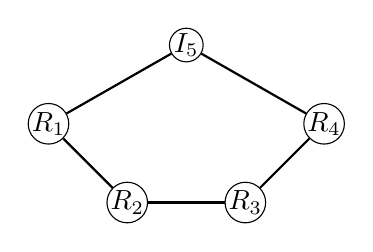
\begin{tikzpicture}[scale=1]
    % Draw a 7,11 network
    % First we draw the vertices
    \foreach \pos/\name in {{(2,3)/R_1}, {(3,2)/R_2}, {(4.5,2)/R_3}, {(5.5,3)/R_4}, {(3.75,4)/I_5}}
        \node[vertex] (\name) at \pos {$\name$};
    
    
    % Connect vertices with edges 
    \foreach \source/ \dest in { R_1/R_2, R_2/R_3, R_3/R_4, R_4/I_5, I_5/R_1}
        \path[edge] (\source) -- (\dest) ;
        
\end{tikzpicture}
\end{center}
\caption{A configuration of the state and the network in which player 1, 2, 3, 4 are Rebels while player 5 is an Inert.}
\label{fig:cyclic_network}
\end{figure}

In Figure~\ref{fig:cyclic_network}, Rebels 2 and 3 are $\theta$-pivotal by definition. From the perspective of Rebel 2, the type of player 5 could be Inert. Therefore, Rebel 2 does not know that Rebel 1 is pivotal. Similarly, Rebel 2 does not know that Rebel 3 is pivotal, \textit{even though} player 3 is indeed $\theta$-pivotal. Therefore there is no common knowledge of the free-rider problem at the beginning of $1$-block. 

However, the common knowledge of engaging in a free-rider problem is restored when we cut the edge between player 4 and 5; Rebel 2 knows that he is the only $\theta$-pivotal Rebel.

I leave a conjecture in this paper and end this section.

\begin{conjecture}
For any $n$-person repeated $k$-Threshold game with parameter $ k < n$ played in any network,
if $\pi$ has full support on strong connectedness, then there exists a $\delta^{*}\in (0,1)$ such that an APEX equilibrium exists whenever $\delta>\delta^{*}$.
\end{conjecture}
%
%
%

\section{Conclusion}
\label{sec:con}

I model a coordination game and illustrate the learning processes generated by strategies in a sequential equilibrium to answer the question proposed in the beginning: what kind of networks can conduct coordination in a collective action with information barrier. In the equilibrium, players transmit the relevant information by encoding such information by their actions as time goes by. Since there might be an negative expected payoff in coding information, the potential free-rider problems might occur to impede the learning process. My result show that if the network is acyclic, players can always learn the underlying relevant information and conduct the coordination only by actions. In cyclic networks, however, what kinds of equilibrium strategies can lead to learning the relevant information still remains to be answered.


The construction of the communication protocol by actions exploits the assumption of the common knowledge of the network and the finite type space. Since the relevant information has been parametrized as a threshold in the stage game, players can acquire this information by jointly incrementally reporting their own private information period by period. The major punishment to deter deviation is then the joint shifting to play that same action as the stopping to update information. The threshold game thus seems a potential model in proofing that a communication protocol by actions not only leads a learning process but also constitutes an equilibrium to reveal the relevant information in finite time.

Existing literatures in political science and sociology have recognized the importance of social network in influencing individual's behavior in participating social movements ( \citep{Passy2003}\citep{McAdam2003}\citep{Siegel2009}). This paper views networks as routes for communication in which rational individuals initially have local information but they can influence nearby individuals by taking actions. Such influence may take long time to travel across individuals and the whole process incurs inefficient outcomes in many periods. A characterization in the speed of information transmission across a network is not answered here, although it is an important topic in investigating the most efficient way to let the information be spread. This question would remain for the future research.



\bibliographystyle{abbrvnat}	% (uses file "plain.bst")
\bibliography{bigref}		% expects file "myrefs.bib"


\appendix
\section{Appendix}
\subsection{The APEX equilibrium for Theorem~\ref{thm_main_result}}
\subsubsection{Equilibrium path}
\label{sec:equilibrium_path}
By definition of information hierarchy, 
\begin{eqnarray*}
I^t_i & = & \bigcup_{k_1\in G_i}\bigcup_{k_2\in G_{k_0}}...\bigcup_{k_{t}\in G_{k_{t-1}}}I^1_{k_{t}}\\
&= & \{v\in [R](\theta): \text{$\exists$ a path $(i,k_1...k_{l},v)$ s.t.~$0\leq l\leq t-1$ and $\theta_i=\theta_{k_1}=...=\theta_{k_l}=R$}\}
\end{eqnarray*}
Let us define several notions.
\begin{notation}[Extended vertices by $I^t_i$]
\label{def:ext_tree}
\begin{eqnarray*}
X^t_i & := &  \{v\in N: \\
	& & \text{$\exists$ a path $(i,k_1...k_{l},k_{l+1})$ s.t.~$k_{l+1}=v$, $l\geq t-1$, $\{i,k_1,...,k_{t}\}\subset I^t_i$}\}\cup I^t_i
\end{eqnarray*}
\end{notation}
Namely, $X^t_i $ is the set of all possible Rebels in $G$ given information $I^t_i$. 

\begin{notation}[The vertices induced by a sub-tree rooting in $j$ but excluding $i$]
\[TR_{ij}:= \{v\in N:\text{there is a path from $i$ to $v$ through $j$}\}\cup\{j\},\text{ where $j\in G_i$}\]
\end{notation}


%\begin{notation}[The vertices that are in $X^t_i$ and $TR_{ij}$, but outside of $I^t_i$]
\begin{notation}[The vertices that are in $X^t_i$ and $TR_{ij}$]
\[Y^t_{ij}:= (X^t_i\cap TR_{ij})\]
\end{notation}


\begin{notation}
\[D^t_{i}:= \{v\in G_i: (Y^t_{ij}\setminus I^t_i)\neq \emptyset\}\]
\end{notation}




\begin{definition}[Finite register machine]
A finite register machine for $i$ consists finite registers $\Sigma$. A register $\sigma\in Sigma$ is a tuple \[(\Omega, \times_{G_i}A_R,f,\lambda),\] in which 
\begin{enumerate}
\item $\Omega$ is the set of all information sets over $\Theta$ induced by $\times^{\infty}_{s=0}H^s_i$. 
\item $\times_{G_i}A_R$ is the set of inputs, which is equal to the set of action profiles of $i$'s neighbors.
\item $f:\Omega\rightarrow A_{R}$ is the outcome function, which maps each information set to an action.
\item $\lambda: \Omega\times \times_{G_i}A_R \rightarrow \Sigma$ is the transition function, which prescribes the transition between registers.
\item There are initial registers. 
\end{enumerate}
\end{definition}

Note that this definition of finite register machine is non-standard in the following sense. An $i$'s register prescribes $i$'s action according to his information at a certain period but does not characterize $i$'s information transition. The information of $i$ up to period $s$ is specified by $P_i(\theta)\times \{h^s_{G_i}\}\times H^s_{N\setminus G_i}$, which is characterized in Section~\ref{sec:model}. 
%The register machine here is more like the \textit{switch function} instead of the finite automata. 

\begin{definition}[$m$-register in $t$-block]
A $m$-register in a (sub)block or a division is the register in the $m$-th period in that (sub)block or division. 
\end{definition}

\begin{notation}[$m\dashv\Gamma$]
\[\text{$m\dashv\Gamma$ is the $m$-register in the (sub)block or division $\Gamma$.}\]
\end{notation}

\begin{definition}[Terminal \textbf{r}]
The terminal \textbf{r} is a register such that the image of $f$ is $\{\textbf{revolt}\}$ and the image of transition $\lambda$ is a singleton containing the register machine itself. 
\end{definition}

\begin{definition}[Terminal \textbf{s}]
The terminal \textbf{s} is a register such that the image of $f$ is $\{\textbf{stay}\}$ and the image of transition $\lambda$ is a singleton containing the register machine itself. 
\end{definition}

The equilibrium will be represented as a {finite register machine}. Note that, though players act as if they are acting a whole sequence, they in fact act period by period. For convenience, for any finite sequence of action $\langle \rangle$, denote $\langle \rangle(m)$ as the $m$-th (counting from the beginning) component in $\langle \rangle$, and denote $\langle \rangle^m$ as the prefix of $\langle \rangle$ with length $m$. If necessary, \textbf{revolt} and \textbf{stay} will be abbreviate as \textbf{r} and \textbf{s} respectively. 

\paragraph{Initial registers}
%\noindent{\textbf{Initial registers}
The initial register for each Rebel is $1\dashv[\Kappa](1)(1,1)$, which is defined in the next section.
\paragraph{Registers in $\Kappa^1$}
%\noindent{\textbf{Equilibrium path in $\Kappa^1$}}

\begin{landscape}
\begin{table}[!htbp]
\caption{The $m\dashv\Kappa^1(1,1)$ on the path}
\label{table:eqm_path_k01}
\begin{center}
\begin{tabular}{c c | c | c | c }
\multicolumn{5}{c}{$1\leq m \leq |\Kappa^1(1,1)|-1$}\\
$\omega_i$ 	 & 	   &	$f(\omega_i)$  &	$a_{G_i}$ & $\lambda(\omega_i,a_{G_i})$ \\
\hline
\hline
$\# X^1_i<k$  	& 	 &$\langle \textbf{all stay} \rangle_m$ &	& terminal \textbf{s}\\
$i\notin R^1$, $\# X^1_i\geq k$, $I^1_i< k$  	&  &$\langle \textbf{all stay} \rangle_m$ & 	& $m+1\dashv\Kappa^1(1,1)$\\
$i\in R^1$, $\# X^1_i\geq k$, $I^1_i< k$  	& 	 &$\langle i \rangle_m$	&  & $m+1\dashv \Kappa^1(1,1)$\\
$i\in R^1$, $\# X^1_i\geq k$, $I^1_i\geq k$  	& 	 &$\langle i \rangle_m$	&  & $m+1\dashv \Kappa^1(1,1)$\\
\hline
\\
\multicolumn{5}{c}{$m=|\Kappa^1(1,1)|$}\\
$\omega_i$ 	 & 	   &	$f(\omega_i)$  &	$a_{G_i}$ & $\lambda(\omega_i,a_{G_i})$ \\
\hline
\hline
$\# X^1_i<k$  	& 	& $\langle \textbf{all stay} \rangle_m$	&     & terminal \textbf{s}\\
$i\notin R^1$, $\# X^1_i\geq k$, $I^1_i< k$   	& all $j$ play $\langle \textbf{all stay} \rangle(m-1)$ & $\langle \textbf{all stay} \rangle_m$	 & all $j$ play \textbf{s} & terminal \textbf{s}\\
$i\notin R^1$, $\# X^1_i\geq k$, $I^1_i< k$   	& $\exists j$ plays $\langle j \rangle(m-1)$ & $\langle \textbf{all stay} \rangle_m$	& such $j$ plays $\langle j \rangle_m$  & $1\dashv \Kappa^1(2,1)$\\
$i\in R^1$, $\# X^1_i\geq k$, $I^1_i< k$   	& 	& $\langle i \rangle_m$	&& $1\dashv \Kappa^1(2,1)$ \\
$i\in R^1$, $\# X^1_i\geq k$, $I^1_i\geq k$  	& 	& $\langle i \rangle_m$ &	& $1\dashv \Kappa^1(2,1)$ \\
\hline
\end{tabular}
\end{center}
\end{table}



\end{landscape}

\begin{landscape}
\begin{table}[!htbp]
\caption{The $m\dashv\Kappa^1(2,1)$ on the path}
\label{table:eqm_path_k02}
\begin{center}
\begin{tabular}{c c | c | c | c}
\multicolumn{5}{c}{$1\leq m < |\Kappa^1(2,1)|$}\\
$\omega_i$ 	 & 	   &	$f(\omega_i)$  &	$a_{G_i}$ & $\lambda(\omega_i,a_{G_i})$ \\
\hline
\hline
$i\notin R^1$  	& & $\langle \textbf{all stay} \rangle_m$	&    & $m+1\dashv \Kappa^1(2,1)$\\
$i\in R^1$, $I^1_i< k$  	& $\exists j\in G_i$, $j$ plays $<j>_j=s$	& $\langle \textbf{all stay} \rangle_m$	& 	& $m+1\dashv \Kappa^1(2,1)$\\
$i\in R^1$, $I^1_i< k$  	& $\forall j\in G_i$, $j$ plays $<j>_j=r$ 	& $\langle i \rangle_m$	& 	& $m+1\dashv \Kappa^1(2,1)$\\
$i\in R^1$, $I^1_i\geq k$  	& 	& $\langle \textbf{all stay} \rangle_m$	&	& $m+1\dashv \Kappa^1(2,1)$\\
\hline
\\
\multicolumn{5}{c}{$m= |\Kappa^1(2,1)|$}\\
$\omega_i$ 	 & 	   &	$f(\omega_i)$  &	$a_{G_i}$ & $\lambda(\omega_i,a_{G_i})$ \\
\hline
\hline
$i\notin R^1$  	& $\forall j\in G_i$, $j$ plays $\langle j \rangle(m-1)$    & $\langle \textbf{all stay} \rangle_m$	& $\forall j\in G_i$, $j$ plays $\langle j \rangle_m$	& $1\dashv \Kappa^1(3,\cdot)$\\
$i\notin R^1$  	& $\exists j\in G_i$, $j$ plays $\langle \textbf{all stay} \rangle(m-1)$   & $\langle \textbf{all stay} \rangle_m$	& such $j$ plays $\langle \textbf{all stay} \rangle_m$	& terminal \textbf{r}\\
$i\in R^1$, $I^1_i< k$   	& $\forall j\in G_i$, $j$ play $\langle j \rangle(m-1)$ 	& $\langle i \rangle_m$	&  $\forall j\in G_i$, $j$ plays $\langle j \rangle_m$	& $1\dashv \Kappa^1(3,\cdot)$ \\
$i\in R^1$, $I^1_i< k$   	&  $\exists j\in G_i$, $j$ plays $\langle \textbf{all stay} \rangle(m-1)$ 	& $\langle i \rangle_m$	& such $j$ plays $\langle \textbf{all stay} \rangle_m$	&  terminal \textbf{r}\\
$i\in R^t$, $I^1_i\geq k$  	& 	& $\langle \textbf{all stay} \rangle_m$	& 	& terminal \textbf{r} \\
\hline
\end{tabular}
\end{center}
\end{table}

\end{landscape}





\begin{table}[!htbp]
\caption{The $m\dashv\Kappa^1(3,\cdot)$ on the path}
\label{table:eqm_path_k03}
\begin{center}
\begin{tabular}{c c | c | c | c}
\multicolumn{5}{c}{$1\leq m < |\Kappa^1(3,\cdot)|$}\\
$\omega_i$ 	 & 	   &	$f(\omega_i)$  &	$a_{G_i}$ & $\lambda(\omega_i,a_{G_i})$ \\
\hline
\hline
  	&	& \textbf{s} & $\forall j$ play $\textbf{s}$ 	& $m+1\dashv \Kappa^1(3,\cdot)$\\
  	&  & \textbf{s}  &  $\exists j$ play $\textbf{r}$  	& terminal \textbf{r}\\
\hline
\\
\multicolumn{5}{c}{$1\leq m = |\Kappa^1(3,\cdot)|$}\\
$\omega_i$ 	 & 	   &	$f(\omega_i)$  &	$a_{G_i}$ & $\lambda(\omega_i,a_{G_i})$ \\
\hline
\hline
  	& 	& \textbf{s} & $\forall j$ play $\textbf{s}$ 	& $1\dashv \Omicron^1$\\
  	&  & \textbf{s}  &  $\exists j$ play $\textbf{r}$  	& terminal \textbf{r}\\
\hline
\end{tabular}
\end{center}
\end{table}



\clearpage

\paragraph{Registers in $\Omicron^t$}
%\noindent \textbf{Equilibrium path in $\Omicron^t$}
In $\Omicron^t$, let $\Omicron^t(m)$ be its $m$-th period. Let $m(I^{t}_i)$ be the period in which $i$ plays $I^t_i$. Formally, $m(I^t_i)$ is a period so that $\langle I^{t}_i \rangle(m(I^t_i))=\textbf{revolt}$. Further define $m(\langle 1 \rangle)=|\Omicron^t|$ and $m(\langle 0 \rangle)=|\Omicron^t|+1$ Then define $G_i(m):=\{j\in G_i: m(I^t_j)<m\}$. Define $I^{t+1}_i(m):= I^t_i\cup(\bigcup_{j\in G_i(m)}I^t_j)$ as the information of $i$ up to the $m$-th period. Define $X^{t+1}_i(m)$ to be the vertices induced by the sub-tree by $I^t_i(m)$ in the same way as that in Definition~\ref{def:ext_tree}, and define $Y^t_{ij}(m)$ and $D^t_i(m)$ accordingly.



%Similarly, define $i$'s extended neighbors to be $G^{t+1}_i(m):= G^t_i\cup(\bigcup_{j\in G_i, m_j<m}I^t_j)$. 




%\noindent \textbf{k-1 Condition} 
%\begin{enumerate}
%\item $\#I^{t+1}_i(m)\geq k-1$
%\item $\#X^{t+1}_i(m)\geq k$
%\item $i$ can tell whether or not $\#[R](\theta)\geq k$ immediately after $\Omicron^t$ whenever none of $i$'s neighbors plays $\langle 1 \rangle$.
%\end{enumerate}

\begin{definition}[Condition $k-1$]
A Rebel $i$ satisfies Condition $k-1$ at the $m$-th period in the reporting phase if
\begin{enumerate}
\item $\#[R](\theta)\geq k\Leftrightarrow\#I^{t+1}_i\geq k$
\item $m(I^t_i)\geq m$
\item $\#I^{t+1}_i(m(I^t_i))\geq k-1$
\end{enumerate}
\end{definition}



%\noindent \textbf{Failure Condition} 
%\begin{enumerate}
%\item $\#X^{t+1}_i(m)< k$ whenever $i$ is inactive
%\end{enumerate}
\begin{definition}[$\theta$ is critical]
Define
\begin{eqnarray*}
\Theta^{<k}_j & := & \{\theta:\text{$j$ is inactive }\Leftrightarrow\#[R](\theta)<k\} \\
\Theta^{k-1}_j & := & \{\theta:\text{$j$ is active }\Rightarrow \text{$j$ satisfies Condition $k-1$}\},
\end{eqnarray*}
for every $j\in [R](\theta)$. Define
\begin{eqnarray*}
\Theta^{\#[R](\theta)<k} & :=  &\bigcup_{j\in [R](\theta)}\Theta^{\#[R](\theta)}_j\\
\Theta^{k-1} & :=  &\bigcup_{j\in [R](\theta)}\Theta^{k-1}_j
\end{eqnarray*}

Then define, \[\text{$\theta$ is \textit{critical} if and only if $\theta\in \Theta^{\#[R](\theta)}\cup \Theta^{k-1}$}\]
\end{definition}






%\noindent \textbf{k-1 Condition} 
%\begin{enumerate}
%\item $\#I^{t+1}_i(m)\geq k-1$
%\item $\#X^{t+1}_i(m)\geq k$
%\item $i$ can tell whether or not $\#[R](\theta)\geq k$ immediately after $\Omicron^t$ whenever none of $i$'s neighbors plays $\langle 1 \rangle$.
%\end{enumerate}

\begin{landscape}
\begin{table}[!htbp]
\caption{The $m\dashv\Omicron^t$ on the path, where $1\leq m < |\Omicron^t|$}
\label{table:eqm_path_ot1}
\begin{center}
\begin{tabular}{c c | c | c | c}
%\multicolumn{5}{c}{$1\leq m < |\Omicron^t|$}\\
$\omega_i$ 	 & 	   &	$f(\omega_i)$  &	$a_{G_i}$ & $\lambda(\omega_i,a_{G_i})$ \\
\hline
\hline
$i\notin R^t$  	& 								& $\langle \textbf{all stay} \rangle_m$		&  			& $m+1\dashv \Omicron^t$ \\
$i\in R^t$, not a free rider, not $k-1$-pivotal		 	&  $\#I^{t+1}_i(m)< k$, $\#X^{t+1}_i(m)<k$			&  $\langle \textbf{all stay} \rangle_m$	& 	& terminal \textbf{s} \\
$i\in R^t$, not a free rider, not $k-1$-pivotal	  	& $\#I^{t+1}_i(m)<k$, $\#X^{t+1}_i(m)\geq k$		    & $\langle I^t_i \rangle_m$ 		&    			& $m+1\dashv \Omicron^t$ \\
$i\in R^t$, not a free rider, not $k-1$-pivotal	 	&  $\#I^{t+1}_i(m)\geq k$, $\#X^{t+1}_i(m)\geq k$	& $\langle 1 \rangle_m$ 	& 	& $m+1\dashv \Omicron^t$ \\
$i\in R^t$, not a free rider, not $k-1$-pivotal	 	&  $\#I^{t+1}_i(m)\geq k-1$, $\#X^{t+1}_i(m)\geq k$, $\#D^t_i=1$	& $\langle 1 \rangle_m$ 	& 	& $m+1\dashv \Omicron^t$ \\
$i\in R^t$, not a free rider, not $k-1$-pivotal	 	&  $\#I^{t+1}_i(m)\geq k-1$, $\#X^{t+1}_i(m)\geq k$, $\#D^t_i>1$	& $\langle I^t_i \rangle_m$ 	& 	& $m+1\dashv \Omicron^t$ \\
$i\in R^t$, the free rider  	&  $\#X^{t+1}_i(m)\geq k$ & $\langle 1 \rangle_m$ 		& 				  & $m+1\dashv \Omicron^t$ \\
$i\in R^t$, the free rider  	&  		$\#X^{t+1}_i(m)<k$					&  $\langle \textbf{all stay} \rangle_m$		& 										  & terminal \textbf{s} \\
$i\in R^t$, $i$ is $k-1$-pivotal  	&  $\#X^{t+1}_i(m)\geq k$ & $\langle 1 \rangle_m$ 	& 											 & $m+1\dashv \Omicron^t$ \\
$i\in R^t$, $i$ is $k-1$-pivotal  	&  	$\#X^{t+1}_i(m)<k$		&  $\langle \textbf{all stay} \rangle_m$	& 											 & terminal \textbf{s} \\
\hline
\end{tabular}
\end{center}
\end{table}


\end{landscape}



\begin{landscape}
\begin{table}[!htbp]
\caption{The $m\dashv\Omicron^t$ on the path, where $m=|\Omicron^t|$}
\label{table:eqm_path_ot2}
\begin{center}
\begin{tabular}{c c | c | c | c}
$\omega_i$ 	 & 	   &	$f(\omega_i)$  &	$a_{G_i}$ & $\lambda(\omega_i,a_{G_i})$ \\
\hline
\hline
%$X^{t+1}_i(m)<k$  	&                                    & 											&				 				& to terminal \textbf{s}\\
$i\notin R^t$  	& 								& $\langle \textbf{all stay} \rangle_m$		&  			& $1\dashv \Kappa^t(1,1)$ \\
$i\in R^t$, not a free rider, not $k-1$-pivotal		 	&  $\#I^{t+1}_i(m)< k$, $\#X^{t+1}_i(m)<k$			&  $\langle \textbf{all stay} \rangle_m$	& 	& terminal \textbf{s} \\
$i\in R^t$, not a free rider, not $k-1$-pivotal	  	& $\#I^{t+1}_i(m)<k-1$, $\#X^{t+1}_i(m)\geq k$		    & $\langle I^t_i \rangle_m$ 		&    			& $1\dashv \Kappa^t(1,1)$ \\
$i\in R^t$, not a free rider, not $k-1$-pivotal	 	&  $\#I^{t+1}_i(m)\geq k$, $\#X^{t+1}_i(m)\geq k$	& $\langle 1 \rangle_m$ 	& 	& $1\dashv \Kappa^t(1,1)$ \\
$i\in R^t$, not a free rider, not $k-1$-pivotal	 	&  $\#I^{t+1}_i(m)\geq k-1$, $\#X^{t+1}_i(m)\geq k$, $\#D^t_i=1$	& $\langle 1 \rangle_m$ 	& 	& $1\dashv \Kappa^t(1,1)$ \\
$i\in R^t$, not a free rider, not $k-1$-pivotal	 	&  $\#I^{t+1}_i(m)\geq k-1$, $\#X^{t+1}_i(m)\geq k$, $\#D^t_i>1$	& $\langle I^t_i \rangle_m$ 	& 	& $1\dashv \Kappa^t(1,1)$ \\
$i\in R^t$, the free rider  	&  $\#I^{t+1}_i(m)\geq k-1$, $\#X^{t+1}_i(m)\geq k$ & $\langle 1 \rangle_m$ 		& 				  & $1\dashv \Kappa^t(1,1)$ \\
$i\in R^t$, the free rider  	&  		$\#X^{t+1}_i(m)<k$					&  $\langle \textbf{all stay} \rangle_m$		& 										  & terminal \textbf{s} \\
$i\in R^t$, $i$ is $k-1$-pivotal  	&  $\#X^{t+1}_i(m)\geq k$ & $\langle 1 \rangle_m$ 	& 											 & $1\dashv \Kappa^t(1,1)$ \\
$i\in R^t$, $i$ is $k-1$-pivotal  	&  	$\#X^{t+1}_i(m)<k$		&  $\langle \textbf{all stay} \rangle_m$	& 											 & terminal \textbf{s} \\
\hline
\end{tabular}
\end{center}
\end{table}


\end{landscape}




\clearpage

\paragraph{Registers in $\Kappa^t$ for $t\geq 2$}
%\noindent \textbf{Equilibrium path in $\Kappa^t$ for $t\geq 1$}
\clearpage
\begin{table}[!htbp]
\caption{The $m\dashv\Kappa^t(1,v)$ for $v=1,...,n$ on the path}
\label{table:eqm_path_kt1}
\begin{center}
\begin{tabular}{c c | c | c | c}
\multicolumn{5}{c}{$1\leq m < |\Kappa^t(1,v)|$, where $v=1,...,n$}\\
$\omega_i$ 	 & 	   &	$f(\omega_i)$  &	$a_{G_i}$ & $\lambda(\omega_i,a_{G_i})$ \\
\hline
\hline
$X^{t+1}_i<k$  	&                                & $\langle \textbf{all stay} \rangle_m$		&				 				& terminal \textbf{s}\\
$X^{t+1}_i\geq k$  	& 						& $\langle i \rangle_m$		&  $\exists j\in G_i, j=m\text{ such that } a_j=\textbf{s}$	& terminal \textbf{s}\\
$X^{t+1}_i\geq k$ 	& 						& $\langle i \rangle_m$		&  $\forall j\in G_i\text{ such that } a_j= \langle j \rangle_m$	& $m+1\dashv \Kappa^t(1,v)$\\
\hline
\\
\multicolumn{5}{c}{$m= |\Kappa^t(1,v)|$, where $v=1,...,n-1$}\\
$\omega_i$ 	 & 	   &	$f(\omega_i)$  &	$a_{G_i}$ & $\lambda(\omega_i,a_{G_i})$ \\
\hline
\hline
$X^{t+1}_i<k$  	&                                & $\langle \textbf{all stay} \rangle_m$	&				 				& terminal \textbf{s}\\
$X^{t+1}_i\geq k$ & 						& $\langle i \rangle_m$		&  $\exists j\in G_i, j=m\text{ such that } a_j=\textbf{s}$	& terminal \textbf{s}\\
$X^{t+1}_i\geq k$ 	& 						& $\langle i \rangle_m$		&  $\forall j\in G_i\text{ such that } a_j= \langle j \rangle_m$	& $1\dashv \Kappa^t(1,v+1)$\\
\hline
\\
\multicolumn{5}{c}{$1\leq m < |\Kappa^t(1,n)|$}\\
\hline
\hline
$X^{t+1}_i\geq k$ 	& 						& $\langle i \rangle_m$		&  $\exists j\in G_i, j=m\text{ such that } a_j=\textbf{s}$	& terminal \textbf{s}\\
$X^{t+1}_i\geq k$ & 						& $\langle i \rangle_m$		&  $\forall j\in G_i\text{ such that } a_j= \langle j \rangle_m$	& $m+1\dashv \Kappa^t(1,n)$\\
\hline
\\
\multicolumn{5}{c}{$m= |\Kappa^t(1,n)|$}\\
$\omega_i$ 	 & 	   &	$f(\omega_i)$  &	$a_{G_i}$ & $\lambda(\omega_i,a_{G_i})$ \\
\hline
\hline
$X^{t+1}_i\geq k$ 	& 						& $\langle i \rangle_m$		&  $\exists j\in G_i, j=m\text{ such that } a_j=\textbf{s}$	& terminal \textbf{s}\\
$X^{t+1}_i\geq k$ 	& 						& $\langle i \rangle_m$		&  $\forall j\in G_i\text{ such that } a_j= \langle j \rangle_m$	& $1\dashv \Kappa^t(2,1)$\\
\hline
\end{tabular}
\end{center}
\end{table}


\clearpage



\begin{table}[!htbp]
\caption{The $m\dashv\Kappa^t(2,v)$ for $v=1,...,t+1$ on the path}
\label{table:eqm_path_kt2}
\begin{center}
\begin{tabular}{c l | c | c | c}
\multicolumn{5}{c}{$1\leq m < |\Kappa^t(2,v)|$, where $v=1,...,t+1$}\\
$\omega_i$ 	 & 	   &	$f(\omega_i)$  &	$a_{G_i}$ & $\lambda(\omega_i,a_{G_i})$ \\
\hline
\hline
$I^{t+1}_i< k$  	& 	$\exists j$, $\langle j \rangle_j=\textbf{s}$	& $\langle \textbf{all stay} \rangle_m$		&  	& $m+1\dashv \Kappa^t(2,v)$\\
$I^{t+1}_i< k$  	& 	$\forall j$, $\langle j \rangle_j=\textbf{r}$	& $\langle i \rangle_m$		&  	& $m+1\dashv \Kappa^t(2,v)$\\
$I^{t+1}_i\geq k$	 & 				& $\langle \textbf{all stay} \rangle_m$ 	& 		& $m+1\dashv \Kappa^t(2,v)$\\
\hline
\\
\multicolumn{5}{c}{$m= |\Kappa^t(2,v)|$, where $v=1,....,t$}\\
$\omega_i$ 	 & 	   &	$f(\omega_i)$  &	$a_{G_i}$ & $\lambda(\omega_i,a_{G_i})$ \\
\hline
\hline
$I^{t+1}_i< k$  	& 	$\exists j\in G_i$, $\langle j \rangle_j=\textbf{s}$	& $\langle \textbf{all stay} \rangle_m$		&  	& $1\dashv \Kappa^t(2,v+1)$\\
$I^{t+1}_i< k$  	& 	$\forall j\in G_i$, $\langle j \rangle_j=\textbf{r}$	& $\langle i \rangle_m$		&  	& $1\dashv \Kappa^t(2,v+1)$\\
$I^{t+1}_i\geq k$	 & 				& $\langle \textbf{all stay} \rangle_m$ 	& 		& $1\dashv \Kappa^t(2,v+1)$\\
\hline
\\
\multicolumn{5}{c}{$1\leq m < |\Kappa^t(2,t+1)|$}\\
$\omega_i$ 	 & 	   &	$f(\omega_i)$  &	$a_{G_i}$ & $\lambda(\omega_i,a_{G_i})$ \\
\hline
\hline
$I^{t+1}_i< k$  	& 	$\exists j\in G_i$, $\langle j \rangle_j=\textbf{s}$	& $\langle \textbf{all stay} \rangle_m$		&  	& $m+1\dashv \Kappa^t(2,t+1)$\\
$I^{t+1}_i< k$  	& 	$\forall j\in G_i$, $\langle j \rangle_j=\textbf{r}$	& $\langle i \rangle_m$		&  	& $m+1\dashv \Kappa^t(2,t+1)$\\
$I^{t+1}_i\geq k$	 & 				& $\langle \textbf{all stay} \rangle_m$ 	& 		& $m+1\dashv \Kappa^t(2,t+1)$\\
\hline
\\
\multicolumn{5}{c}{$m= |\Kappa^t(2,t+1)|$}\\
$\omega_i$ 	 & 	   &	$f(\omega_i)$  &	$a_{G_i}$ & $\lambda(\omega_i,a_{G_i})$ \\
\hline
\hline
$I^{t+1}_i< k$  	& 	$\exists j\in G_i$, $\langle j \rangle_j=\textbf{s}$	& $\langle \textbf{all stay} \rangle_m$		&  	& terminal \textbf{r}\\
$I^{t+1}_i< k$  	& 	$\forall j\in G_i$, $\langle j \rangle_j=\textbf{r}$	& $\langle i \rangle_m$		&  	& $1\dashv \Kappa^t(3,1)$\\
$I^{t+1}_i\geq k$	 & 				& $\langle \textbf{all stay} \rangle_m$ 	& 		& terminal \textbf{r}\\
\hline
\end{tabular}
\end{center}
\end{table}




\clearpage









\begin{table}[!htbp]
\caption{The $m\dashv\Kappa^t(3,1)$ on the path}
\label{table:eqm_path_kt3}
\begin{center}
\begin{tabular}{c c | c | c | c}
\multicolumn{5}{c}{$1\leq m < |\Kappa^t(3,1)|$}\\
$\omega_i$ 	 & 	   &	$f(\omega_i)$  &	$a_{G_i}$ & $\lambda(\omega_i,a_{G_i})$ \\
\hline
\hline
  	&	& \textbf{s} & $\forall j\in G_i$, $j$ plays $\textbf{s}$ 	& $m+1\dashv \Kappa^t(3,1)$\\
  	&  & \textbf{s}  &  $\exists j\in G_i$, $j$ plays $\textbf{r}$  	& terminal \textbf{r}\\
\hline
\\
\multicolumn{5}{c}{$m= |\Kappa^t(3,1)|$}\\
$\omega_i$ 	 & 	   &	$f(\omega_i)$  &	$a_{G_i}$ & $\lambda(\omega_i,a_{G_i})$ \\
\hline
\hline
 	& 	& \textbf{s} & $\forall j\in G_i$, $j$ plays $\textbf{s}$ 	& $1\dashv \Omicron^{t+1}$\\
  	&  & \textbf{s}  &  $\exists j\in G_i$, $j$ play $\textbf{r}$  	& terminal \textbf{r}\\
\hline
\end{tabular}
\end{center}
\end{table}




\clearpage
\subsection{Missing proofs}
%\label{appx_network}
\noindent\textbf{Proof of Lemma~\ref{lemma_learn}}
%\begin{lemma*}[Learning in the APEX equilibrum]
%If the assessment $(\tau^*,\mu^{*})$ is an APEX equilibrium, then for all $\theta\in \Theta$, there is a finite time $T^{\theta}_i$ for every Rebel $i$ such that $\sum_{\theta\in\{\theta:[R](\theta)\geq k\}}\beta^{\pi,\tau^*}_{G_i}(\theta|h^{s}_{G_i})=$ either $1$ or $0$
%whenever $s\geq T^{\theta}_i$.
%\end{lemma*}
\begin{proof}
The proof is done by contraposition. Suppose Rebels' strategies constitute an APEX equilibrium. By definition of the APEX equilibrium, at every $\theta$, there is a period $T^{\theta}$ when all Rebels' actions start to repeat themselves. Let $T=\max_{\theta\in \Theta}{T^{\theta}}$. For Rebel $i$, let $T_i=T+1$, and suppose $0<\sum_{\theta:\#[R](\theta)\geq k}\beta^{\pi,\tau^*}_{G_i}(\theta|h^{s}_{G_i})<1$ for some $s\geq T_i$. Then this Rebel assigns positive weight at some ${\theta^{'}}\in \{\theta:\#[R](\theta)< k\}$ and some positive weight at some ${\theta^{''}}\in \{\theta:\#[R](\theta)\geq k\}$ at period $s$. Note that $i$ has already known $\theta_j$ if $j\in G_i$, and therefore $i$ assigns positive weight at some $\theta^{'}\in \{\theta:\#[R](\theta)< k, \theta_l=R, l\notin G_i\}$ and positive weight at some $\theta^{''}\in \{\theta:\#[R](\theta)< k, \theta_l=I, l\notin G_i\}$. Since all Rebels' actions start to repeat themselves at period $T$, $i$ cannot update information afterwards. Suppose $i$'s continuation strategy is to continuously play \textbf{revolt}, then this is not ex-post efficient when $\#[R](\theta)< k$. Suppose $i$'s continuation strategy is to continuously play \textbf{stay}, then this is not ex-post efficient when $\#[R](\theta)\geq k$.
\end{proof}
%
%
\bigskip
\noindent\textbf{Proof of Theorem~\ref{thm_minor_thm}}
%\begin{theorem*}[APEX equilibrium for the case of $k=n$]
%For any $n$-person repeated $k$-Threshold game with parameter $k=n$ played in a network, there is a $\delta^{*}$ such that a sequential APEX equilibrium exists whenever $\delta>
%\delta^{*}$.
%\end{theorem*}
\begin{proof}
Let $\tau^{*}$ be the following strategy. After the nature moves, a Rebel $i$ plays \textbf{revolt} if he has no Inert neighbor, and plays \textbf{stay} forever if he has an Inert neighbor. After the first period, if $i$ has not detect a deviation and observes that all his Rebel neighbors play \textbf{revolt} continuously previously, he will play \textbf{revolt} in the current period; otherwise, he will play \textbf{stay} afterwards and forever. If a Rebel $j$ deviates, then $j$ plays \textbf{stay} afterwards and forever.

At period $s$, according to $\tau^{*}$, if $i$ has not detect a deviation, but observes that his Rebel neighbors play \textbf{stay} in the current period, he will form the belief of \[\sum_{\theta:\#[R](\theta)\geq k}\beta^{\pi,\tau^*}_{G_i}(\theta|h^{s}_{G_i})=0\] afterwards and forever. Therefore, he plays \textbf{stay} afterwards and forever as his best response. 

At period $s$, if a Rebel detects a deviation or has deviated, then to play \textbf{stay} afterwards and forever is his best response since at least one player will play \textbf{stay} afterwards and forever. 

Since the network is finite with $n$ vertices, if all players do not deviate, after period $n$, each Rebel plays \textbf{revolt} and get payoff $1$ forever if $\theta\in \{\theta: \#[R](\theta)\geq k\}$ or plays \textbf{stay} and gets payoff $0$ forever if $\theta\in \{\theta: \#[R](\theta)< k\}$. However, a Rebel who has deviated surely gets payoff $0$ forever after period $n$. Therefore, there is a $0<\delta<1$ large enough to impede Rebels to deviate.

To check if $\tau^{*}$ and $\{\beta^{\pi,\tau^*}_{G_i}(\theta|h^{s}_{G_i})\}_{i\in N}$ satisfy full consistency\footnote{Krep and Wilson (1982)}, take any $0<x<1$ such that Rebels play $\tau^{*}$ with probability $1-x$ and play other behavior strategies with probability $x$. Clearly, when $x \rightarrow 0$, the belief converges to $\{\beta^{\pi,\tau^*}_{G_i}(\theta|h^{s}_{G_i})\}_{i\in N}$. Since the off-path strategy is the best response for both the Rebel who detects deviation and the Rebel who deviates, for the arbitrary beliefs they hold, $\tau^{*}$ is a sequential equilibrium.
\end{proof}
%
%
%\bigskip
%\noindent\textbf{Proof of Lemma~\ref{lemma_inclusion}}
%%\begin{lemma*}
%%%\label{lemma_inclusion}
%%If the $\theta$ has strong connectedness, then 
%%\[R^t\subseteq R^{t-1}\] for all $t\geq 1$
%%\end{lemma*}
%\begin{proof}
%I show that if $i\notin R^{t-1}$ then $i\notin R^t$ for all $t$. 
%
%By definition, 
%\begin{eqnarray*}
%G^t_i & = & \bigcup_{k_1\in G_i}\bigcup_{k_2\in G_{k_0}}...\bigcup_{k_{t}\in G_{k_{t-1}}}G^{1}_{k_{t}}\\
%&= & \{j\in N: \text{$\exists$ a path $(i,k_1...k_{l},j)$ such that $l\leq t-1$ and $\theta_i=\theta_{k_1}=...=\theta_{k_l}=R$}\},
%\end{eqnarray*}
%while
%\begin{eqnarray*}
%I^t_i & = & \bigcup_{k_1\in G_i}\bigcup_{k_2\in G_{k_0}}...\bigcup_{k_{t}\in G_{k_{t-1}}}I^{1}_{k_t}\\
%&= & \{j\in [R](\theta): \text{$\exists$ a path $(i,k_1...k_{l},j)$ such that $l\leq t-1$ and $\theta_i=\theta_{k_1}=...=\theta_{k_l}=R$}\}.
%\end{eqnarray*}
%The above equality says that, at $t=\dot{t}$, if $i\notin R^{\dot{t}}$, then there is a $j$ such that the Rebels, who can be reached by $\dot{t}$ consecutive edges from $i$, can be also reached by $\dot{t}$ consecutive edges from $j$. Therefore, if there are new Rebels who can be reached from $i$ at any $\ddot{t}>\dot{t}$ by $\ddot{t}$ consecutive edges, those new ones can be also be reached by $\ddot{t}$ consecutive edges by $j$. Hence, $i\notin R^{\ddot{t}}$. 
%\end{proof}



%
\bigskip
\noindent\textbf{Proof of Theorem~\ref{lemma_empty}}
%\begin{lemma*}
%If the network is acyclic and if the $\theta$ has strong connectedness, then 
%\[[R](\theta)\neq \emptyset \Rightarrow \text{ there exists } t\geq 0 \text{ and } i\in R^t \text{ such that }I^{t+1}_i=[R](\theta).\] 
%\end{lemma*}
\begin{proof}

%\begin{definition}[A tree rooted in $i$ and spanning in the direction toward $j$]
%\[TR_{ij}:= \{v\in N:\text{there is a path from $i$ to $v$ through $j$}\}.\]
%\end{definition}


Since the network is finite, $\theta$ has strong connectedness, and $[R](\theta)\neq \emptyset$, there is a minimum $t_i$ such that $I^{t_i}_i=[R](\theta)$ for each $i$ by the definition of $I^t_i$. Let $P=\underset{i\in N}{\arg\min}\{t_i\}$ with generic element $p$. Therefore $I^{t_p}_p=[R](\theta)$. I show that $p\in R^{t_p-1}$ to complete the proof. I prove it by contradiction. If $p\notin R^{t_p-1}$, then $I^{t_p-1}_p\subseteq G^{t_p-1}_j$ for some $j\in G_p$. Then, all the Rebels in $TR_{jp}$ are in $G^{t_p-1}_j$, but there exist Rebels in $TR_{pj}$ who are in $G^{t_p-1}_j$ but not in $I^{t_p-1}_p$. This is because the network is acyclic and $I^{t_p-1}_p\subset [R](\theta)$. But then $p\notin P$ since $I^{t_j-1}_j=[R](\theta)$ already. I then conclude that $p\in R^{t_p-1}$.

\end{proof}





\noindent\textbf{Proof of Lemma~\ref{lemma_at_most_two_nodes}} 
%\begin{lemma*}
%If the network is acyclic and if $\pi$ has full support on strong connectedness, then for each $t$-block, there are at most two $\theta$-pivotal Rebels. Moreover, if there are two of them, they are neighbors.\footnote{As a remark, the above lemma is not true when the network is cyclic. To see this, consider a 4-player circle when $\theta=(R,R,R,R)$.}
%\end{lemma*}
   
\begin{proof}
The proof is by contradiction. Suppose that, at $t$-block and before $T^{\theta}$, there are three or more active $\theta$-pivotal Rebels. Since $\theta$ has strong connectedness, there are three of them, $p_1,p_2,p_3$, with the property $p_1\in G_{p_2}$ and $p_2 \in G_{p_3}$. 

Since the network is acyclic, $p_1\notin G_{p_3}$ and $p_3\notin G_{p_1}$. Since $p_1$ is an active $\theta$-pivotal Rebel, $p_1$ is uncertain  $I^t_{p_1}= [R](\theta)$ and certain $I^{t+1}_{p_1}=[R](\theta)$. This implies that, in $TR_{p_1p_2}$, $p_1$ can reach all Rebels by $t+1$ edges, but might not reach all of them by $t$ edges. The same situation applies to $p_3$. However, this means that $p_2$ can reach all Rebels in $TR_{p_1p_1}$ by $t$ edges and reach all Rebels in $TR_{p_1p_1}$ by $t$ edges, and hence $p_2$ is certain $I^t_{p_2}=[R](\theta)$ at $t$-block. It contradicts to the definition of the $\theta$-pivotal Rebel.

\end{proof}



\bigskip
\noindent\textbf{Proof of Lemma~\ref{lemman_pivotals_CK}}
%\begin{lemma*}
%If the network is acyclic and if $\pi$ has full support on strong connectedness, then for each $t$-block, if there are two $\theta$-pivotal Rebels $p$ and $p^{'}$, then they commonly know that they are $\theta$-pivotal Rebels at the beginning of $t$-block.
%\end{lemma*}
\begin{proof}
Since there are two active $\theta$-pivotal Rebels and since the network is acyclic, all Rebels in $TR_{p{'}p}$ is in $I^t_{p}$, and all Rebels in $TR_{pp^{'}}$ is in $I^t_{p^{'}}$. Moreover, all vertices in $Y^t_{p^{'}p}$ can be reached by $t+1$ edges from $p^{'}$, and all vertices in $Y^t_{pp^{'}}$ can be reached by $t+1$ edges from $p$. Furthermore, some vertices in $Y^t_{p^{'}p}$ must only be reached by $t+1$ edges from $p^{'}$, and some vertices in $Y^t_{pp^{'}}$ must only be reached by $t+1$ edges from $p$. 

By the network being commonly known, $p$ is therefore certain that he himself is $\theta$-pivotal by concluding it might be $I^t_{p}\subset [R](\theta)$ and $I^{t+1}_{p}=[R](\theta)$. By the network being commonly known and $p$ being active, $p$ is certain that $p^{'}$ is $\theta$-pivotal by concluding $I^t_{p^{'}}\subset [R](\theta)$ and $I^{t+1}_{p^{'}}=[R](\theta)$. The above arguments hold true for $p^{'}$ by replacing $p$ by $p^{'}$ and $p^{'}$ by $p$. Then $p$ and $p^{'}$ commonly know that they are $\theta$-pivotal by applying the common knowledge of network. Note that, though, they are uncertain whether they are both active.
\end{proof}
\bigskip


\noindent\textbf{Proof of Lemma~\ref{lemma_at_most_two_1edges}} 
%\begin{lemma*}
%If the network is acyclic and if $\pi$ has full support on strong connectedness, then for each $t$-block, there are at most two $\theta$-pivotal Rebels. Moreover, if there are two of them, they are neighbors.\footnote{As a remark, the above lemma is not true when the network is cyclic. To see this, consider a 4-player circle when $\theta=(R,R,R,R)$.}
%\end{lemma*}
   
\begin{proof}
The proof is by contradiction. Suppose that, at $t$-block and before $T^{\theta}$, there are three or more active 1-edge-$\theta$-pivotal Rebels. Since $\theta$ has strong connectedness, there are three of them, $p_1,p_2,p_3$, with the property $p_1\in G_{p_2}$ and $p_2 \in G_{p_3}$. 

Since the network is acyclic, $p_1\notin G_{p_3}$ and $p_3\notin G_{p_1}$. Since $p_1$ is an active 1-edge-$\theta$-pivotal Rebel, $p_1$ is uncertain  $I^{t+1}_{p_1}= [R](\theta)$ and certain $I^{t+2}_{p_1}=[R](\theta)$. This implies that, in $TR_{p_1p_2}$, $p_1$ can reach all Rebels by $t+2$ edges, but might not reach all of them by $t+1$ edges. The same situation applies to $p_3$. However, this means that $p_2$ can reach all Rebels in $TR_{p_1p_1}$ by $t+1$ edges and reach all Rebels in $TR_{p_1p_1}$ by $t+1$ edges, and hence $p_2$ is certain $I^{t+1}_{p_2}=[R](\theta)$ at $t$-block. It contradicts to the definition of the 1-edge-$\theta$-pivotal Rebel.

\end{proof}
\bigskip

\bigskip
\noindent\textbf{Proof of Lemma~\ref{lemman_1edge_pivotals_CK}}
%\begin{lemma*}
%If the network is acyclic and if $\pi$ has full support on strong connectedness, then for each $t$-block, if there are two $\theta$-pivotal Rebels $p$ and $p^{'}$, then they commonly know that they are $\theta$-pivotal Rebels at the beginning of $t$-block.
%\end{lemma*}
\begin{proof}
Since there are two active 1-edge-$\theta$-pivotal Rebels and since the network is acyclic, all Rebels in $TR_{p{'}p}$ is in $I^{t+1}_{p}$, and all Rebels in $TR_{pp^{'}}$ is in $I^{t+1}_{p^{'}}$. Moreover, all vertices in $Y^t_{p^{'}p}$ can be reached by $t+2$ edges from $p^{'}$, and all vertices in $Y^t_{pp^{'}}$ can be reached by $t+2$ edges from $p$. Furthermore, some vertices in $Y^t_{p^{'}p}$ must only be reached by $t+2$ edges from $p^{'}$, and some vertices in $Y^t_{pp^{'}}$ must only be reached by $t+2$ edges from $p$. 

By the network being commonly known, $p$ is therefore certain that he himself is 1-edge-$\theta$-pivotal by concluding it might be $I^{t+1}_{p}\subset [R](\theta)$ and $I^{t+2}_{p}=[R](\theta)$. By the network being commonly known and $p$ being active, $p$ is certain that $p^{'}$ is 1-edge-$\theta$-pivotal by concluding $I^{t+1}_{p^{'}}\subset [R](\theta)$ and $I^{t+2}_{p^{'}}=[R](\theta)$. The above arguments hold true for $p^{'}$ by replacing $p$ by $p^{'}$ and $p^{'}$ by $p$. Then $p$ and $p^{'}$ commonly know that they are 1-edge-$\theta$-pivotal by applying the common knowledge of network. Note that, though, they are uncertain whether they are both active.
\end{proof}
\bigskip








\noindent\textbf{Proof of Theorem~\ref{thm_main_result}}
I begin with the following lemmas stating that all Rebels eventually learn the relevant information on the path.
\begin{lemma}
\label{lemma:learning_on_the_path}
If the network is acyclic and if the $\theta$ has strong connectedness, then the equilibrium path prescribed in Section~\ref{sec:equilibrium_path} is an APEX strategy.
\end{lemma}
\begin{proof}
Firstly, suppose $\theta$ satisfies $\#[R](\theta)<k$. I show that, all Rebels will enter terminal \textbf{s} eventually without entering terminal \textbf{r}.  Let $p$ be the Rebel defined in the proof of Theorem~\ref{lemma_empty} so that $I^{t_p}_p=[R](\theta)$, where $p$ is one of the earliest Rebels who knows $\#[R](\theta)<k$. I claim that $\#X^{t_p}_p< k$ if and only if $I^{t_p}_p=[R](\theta)$. For the "only if'' part, the proof is by way of contradiction. If not, by the full support of strong connectedness, there is a possible Rebel outside $I^{t_p}_p$ , and therefore $p$ is uncertain that $\#[R](\theta)<k$. For the "if" part, note that $I^{t_p}_p\subset X^{t_p}_p$ and therefore $\#I^{t_p}_p< \#X^{t_p}_p<k$. I also claim that $\#X^{t_p}_p(m)<k$ if and only $I^{t_p}_p(m)=[R](\theta)$. The proof is exactly the same as the noted above by replacing $I^{t_p}_p$ to $I^{t_p}_p$ and $I^{t_p}_p(m)$ to $I^{t_p}_P(m)$.

Referring to Table~\ref{table:eqm_path_k01} to Table~\ref{table:eqm_path_ot2}, whenever there is a $p$ so that $\#X^{t_p}_p<k$, $p$ plays \textbf{stay} forever. It implies that all Rebels enter terminal \textbf{s} right after $\Kappa^t_1, t\geq 0$. Notice that Rebels enter terminal \textbf{r} only after some period after $\Kappa^t_1$ and therefore all Rebels will enter terminal \textbf{s} before terminal \textbf{r}. 

Secondly, suppose $\theta$ satisfies $\#[R](\theta)\geq k$. I show that all Rebels will enter terminal \textbf{r} eventually. Note first that if there is a Rebel $p$ that $\#I^1_p\geq k$, all Rebels enter terminal \textbf{r} after $\Kappa^1(3,\cdot)$ referring to Table~\ref{table:eqm_path_k01}, Table~\ref{table:eqm_path_k02}, and Table~\ref{table:eqm_path_k03}. At $t>0$, if there is a Rebel $p$ who has played $\langle 1 \rangle$ at $\Omicron^t$, by the postulate of $\#[R](\theta)\geq k$, after $\Kappa^t(3,\cdot)$, all Rebels enter terminal \textbf{r} according to the equilibrium path prescribed in Table~\ref{table:eqm_path_ot1}, Table~\ref{table:eqm_path_ot2}, Table~\ref{table:eqm_path_kt1}, Table~\ref{table:eqm_path_kt2}, and Table~\ref{table:eqm_path_kt3}. There must be some Rebel $p\in R^t$ who plays $\langle 1 \rangle$ at $\Omicron^t$ for some $t$ by the same argument in the proof of Theorem~\ref{lemma_empty}.
%a $\theta$-pivotal or whose $I^{t+1}_p(m)\geq k-1, D^t_p(m)=1$, then $p$ plays $\langle 1 \rangle$. If $p$ is a free rider or is a single $\theta$-pivotal, his neighbor will report truthful information or $\langle 1 \rangle$ to him. Thus he will know $\#[R](\theta)\geq k$ after $\Omicron^t$. If $p$ has $I^{t+1}_p(m)\geq k-1$ but $\#X^{t+1}_p(m)\geq k$, there are two cases. The first case is there is Rebel neighbor $j$ will report some $I^t_j$ such that $\# I^t_j\setminus I^{t+1}_p(m)\geq 1$ by the postulate of $\#[R](\theta)\geq k$, $\#X^{t+1}_p(m)\geq k$, and the full support on strong connectedness. The second case is there is Rebel neighbor $j$ who plays $\langle 1 \rangle$. The first case implies $\#I^{t+1}_p\geq k$. The second case implies $\#I^{t+1}(m)_p\geq k-1$ and $I^{t+1}(m)_p\geq k-1$, and hence $I^{t+1}_i\geq k$ if the network is acyclic. 
%In either case, after $\Kappa^t(3,\cdot)$, all Rebels enter terminal \textbf{r} according to the equilibrium path prescribed in Table~\ref{table:eqm_path_ot1}, Table~\ref{table:eqm_path_ot2}, Table~\ref{table:eqm_path_kt1}, Table~\ref{table:eqm_path_kt2}, and Table~\ref{table:eqm_path_kt3}. 
\end{proof}


%Due to Lemma~\ref{lemma:learning_on_the_path}, define $T^{\theta}_{\tau^{*}}$ as the earliest period at which all Rebels play ex-post efficient outcome afterwards according to an APEX equilibrium $\tau^{*}$.  I prepare the following claims to proceed the proof. These claims will hold for $\pi$ having full support on strong connectedness. For conciseness, in the following claims, I only consider non-trivial cases. I only consider $2<k<n$ as aforementioned and the period $s$ when $s<T^{\theta}_{\tau^{*}}$. For the case of $s>T^{\theta}_{\tau^{*}}$, it should be clear that Rebels will not deviate from the equilibrium path.\footnote{This is because the ex-post efficient outcome in the $k$-threshold game is being played if $s>T^{\theta}_{\tau^{*}}$.}
%Furthermore, I only consider the case that $i$ still believes $\#[R](\theta)\geq k$ with positive probability. Otherwise $i$ will play \textbf{stay} forever on the equilibrium path. 
%
%Some notations are introduced. I suppress the notation $\beta^{\pi,\tau}_{G_i}(\theta|h^s_{G_i})$ to $\beta^{\tau}_{G_i}(\theta|h^s_{G_i})$ and the notation $\alpha^{\pi,\tau}_{G_i}(\theta, h^{s}|\theta_{G_i},h^{s}_{G_i})$ to $\alpha^{\tau}_{G_i}(\theta, h^{s}|h^{s}_{G_i})$. If $\mathbf{Prop}(\theta)$ is a property of $\theta$, define \[\beta^{\tau}_{G_i}(\mathbf{Prop}(\theta)|h^s_{G_i}):= \sum_{\theta\in\{\theta:\mathbf{Prop}(\theta)\}}\beta^{\tau}_{G_i}(\theta|h^s_{G_i}).\] Furthermore, if $s^{'}$ and $s$ are periods and $s^{'}>s$, denote $h^{s^{'}|s}$ as a history in $H^{s^{'}}$ so that $(h^s,h^{s^{'}|s})\in H^{s^{'}}$. Denote $\tau^{'}|^s_{\tau}$ as a strategy following $\tau$ till period $s$. Finally, define
%\[
%    I^s_i:=\left\{
%                \begin{array}{lcl}
%                  I^{t+1}_i(m) & \text{if} & s\in \Omicron^t, s=m+\sum^t_{\gamma=1}(|\Kappa^{\gamma}|+|\Omicron^{\gamma-1}|).\\
%                 I^{t}_i & \text{if} & s\in \Kappa^t.
%                \end{array}
%              \right. 
%\]

%The central idea of the following claims is

\begin{lemma}
\label{lemma:uncertain}
Let Rebel $i$ follow the constructed APEX equilibrium $\tau^{*}$ till period $s$ so that $0<\beta^{\tau^{*}}_{G_i}(\#[R](\theta)\geq k|h^s_{G_i})<1$.
\begin{enumerate}[label=(\arabic*)]
\item If $\tau|^s_{\tau^{*}}$ is a continuation strategy that induces $i$ to be uncertain about the relevant information and stop belief-updating after some period $s^{'}$, then $i$ will not deviate to $\tau|^s_{\tau^{*}}$ given sufficient high $\delta$.
\item If $0<\beta^{\tau^{*}}_{G_i}(\#[R](\theta)\geq k|h^s_{G_i})\leq1$ and $\tau|^s_{\tau^{*}}$ is a continuation strategy that generates the stage payoff at most 0 after some period $s^{'}$ conditional on an event $E$, where 
\[E\subseteq \mathrm{supp}(\beta^{\tau^{*}}_{G_i}(\cdot |h^s_{G_i}))\cap\{\theta^{'}:\#[R](\theta^{'})\geq k\},\] 
then $i$ will not deviate to $\tau|^s_{\tau^{*}}$ given sufficient high $\delta$.
\item If $s$ is after $\Kappa^1$, then $i$ is certain that any Rebel has less than $k$ Rebel neighbors.
\item If $s$ is after $\Kappa^1$ and $\tau|^s_{\tau^{*}}$ is a continuation strategy that generates detectable deviations at $s$ or afterwards, then $i$ will not deviate to $\tau|^s_{\tau^{*}}$ given sufficient high $\delta$.
\item If $s$ is in $\Kappa^1$ and $\tau|^s_{\tau^{*}}$ is a continuation strategy that generates detectable deviations at $s$, then $i$ will not deviate to $\tau|^s_{\tau^{*}}$ given sufficient high $\delta$.
\end{enumerate}

\end{lemma}
\begin{proof}
Due to Lemma~\ref{lemma:learning_on_the_path}, it is safe to define $T^{\theta}_{\tau^{*}}$ as the earliest period at which all Rebels play ex-post efficient outcome afterwards according to an APEX equilibrium $\tau^{*}$. 
The proof for each claim proceeds as follows. 
\begin{enumerate}[label=(\arabic*)]
\item Denote $h^{s^{'}|s}$ as a history in $H^{s^{'}}$ so that $(h^s,h^{s^{'}|s})\in H^{s^{'}}$ when $s^{'}>s$. Denote $\beta^{\tau|^s_{\tau^{*}}}_{G_i}(\theta|h^{s^{'}|s}, h^s_{G_i})$ as $i$'s belief about $\theta$ at $s^{'}$ following $h^{s^{'}|s}$ induced by $\tau|^s_{\tau^{*}}$. By the postulate,  $0<\beta^{\tau|^s_{\tau^{*}}}_{G_i}(\#[R](\theta)|h^{s^{'}|s}, h^s_{G_i})<1$. From the perspective that $i$ holds a belief of $0<\beta^{\tau^{*}}_{G_i}(\#[R](\theta)\geq k|h^s_{G_i})<1$ at period $s$, $h^{s^{'}|s}$ can be thought of a signal at period $s^{'}$ to infer whether or not $\#[R](\theta)\geq k$: if $\#[R](\theta)\geq k$, $h^{s^{'}|s}$ occurs with probability $\eta$ and does not occur with probability $1-\eta$, or if $\#[R](\theta)< k$, $h^{s^{'}|s}$ occurs with probability $\mu$ and does not occur with probability $1-\mu$, subject to $0\leq \eta \leq 1$, $0\leq\mu\leq 1$ and $0<\eta/\mu<\infty$. The last inequality follows the postulate that $h^{s^{'}|s}$ is generated with positive probability by $\tau|^s_{\tau^{*}}$. Denote $S=\max\{s^{'}, T^{\theta}_{\tau^{*}}\}$. Following $h^{s^{'}|s}$, Rebel $i$'s maximum expected stage-game payoff starting from $S$ and calculated at period $s$ is 
\[w=\max\{\eta\beta^{\tau^{*}}_{G_i}(\#[R](\theta)\geq k|h^s_{G_i})-\mu\beta^{\tau^{*}}_{G_i}(\#[R](\theta)< k|h^s_{G_i}),0\}.\]
The first term of the above bracket, $\eta\beta^{\tau^{*}}_{G_i}(\#[R](\theta)\geq k|h^s_{G_i})-\mu\beta^{\tau^{*}}_{G_i}(\#[R](\theta)< k|h^s_{G_i})$, is $i$'s expected stage-game payoff if all Rebels play \textbf{revolt} afterwards starting from $S$.  The second term $0$ is $i$'s individual rational payoff by playing \textbf{stay} afterwards. Rebel $i$'s expected stage-game payoff starting from $S$ on the path, in present value, is 
\[\beta^{\tau^{*}}_{G_i}(\#[R](\theta)\geq k|h^s_{G_i}).\] 
Note that
\[\beta^{\tau^{*}}_{G_i}(\#[R](\theta)\geq k|h^s_{G_i})>w.\]
The inequality above is due to $0\leq \eta \leq 1$, $0\leq\mu\leq 1$ and $0<\eta/\mu<\infty$ by the postulate. There is a loss in present value of
\[v(\delta)=\frac{\delta^{S-s}(\beta^{\tau^{*}}_{G_i}(\#[R](\theta)\geq k|h^s_{G_i})-w)}{1-\delta},\]
comparing to the equilibrium path. Denote $z$ as the summation of all gains from deviation calculated from period $s$ to period $S$. $z$ is finite since the stage-game payoff is finite and $S-s$ is finite. Taking sufficiently high $\delta$ so that $v(\delta)>z$ will deter this deviation.

\item On the path, for every $\theta^{'}\in \mathrm{supp}(\beta^{\tau^{*}}_{G_i}(\cdot |h^s_{G_i}))$, $i$ will get the highest stage payoff as 1 at every period after $T^{\theta^{'}}_{\tau^{*}}$. Denote $S=\max\{s^{'}, T^{\theta}_{\tau^{*}}\}$. If $i$ deviates to $\tau$, comparing to the equilibrium path, there is a loss in expected payoff in present value at least 
\[v(\delta, E)\geq k)=\frac{\delta^{S-s}}{1-\delta}\] 
conditional on $E$. Conditional on $\mathrm{supp}(\beta^{\tau^{*}}_{G_i}(\cdot |h^s_{G_i}))\setminus E$, comparing to the equilibrium path, $i$'s expected gain in present value is at most $z<\infty$ by taking all gains from period $s$ to period $S$. Taking sufficiently high $\delta$ so that $v(\delta, \#[R](\theta)\geq k)>z$ will deter $i$'s deviation.
\item The proof is done by contradiction. If there is a Rebel who has at least $k$ Rebel neighbors, by tracking the equilibrium path, $T^{\theta}_{\tau^{*}}$ arrives in $\Kappa^1$. Then, by Lemma~\ref{lemma_learn} and Lemma~\ref{lemma:learning_on_the_path}, $\beta^{\tau^{*}}_{G_i}(\#[R](\theta)\geq k|h^s_{G_i})=0$ or $=1$ if $s$ is after $\Kappa^1$. It contradicts the postulate that $0<\beta^{\tau^{*}}_{G_i}(\#[R](\theta)\geq k|h^s_{G_i})<1$.
\item This claim is a consequence of (2) and (3). Since $s$ is after $\Kappa^1$, $i$ is certain that any Rebel has less than $k$ Rebel neighbors by (3). Since that, $i$'s detectable deviations will let the detectors play \textbf{stay} forever by their off-path belief for every $\theta^{'}\in \mathrm{supp}(\beta^{\tau^{*}}_{G_i}(\cdot |h^s_{G_i}))$. Let $d\geq 1$ be the number of detectors. Since $0<\beta^{\tau^{*}}_{G_i}(\#[R](\theta)\geq k|h^s_{G_i})<1$, there exists an event $E$ and $d\geq 1$ so that
\[E=\mathrm{supp}(\beta^{\tau^{*}}_{G_i}(\cdot |h^s_{G_i}))\cap \{\theta:k+d>\#[R](\theta)\geq k\}.\] 
Conditional on $E$, following $\tau|^s_{\tau^{*}}$, $i$'s stage payoff is at most 0 after period $s^{'}$. This is because no more than $k$ Rebels will choose \textbf{revolt} after $s^{'}$ by $\#[R](\theta)-d<k$. This claim is then proved by applying (2).
\item In this case, in contrast to (3), there might be a Rebel who has at least $k$ Rebel neighbors on the path. The proof for (4) does not directly applies here. The proof for this claim will respectively considers $i$ being an active Rebel or an inactive one. 

Firstly suppose $i$ is active. Since $i$ is active, for every $j\in G_i$, there is a Rebel outside $G^1_j=G_j$ and therefore outside $I^1_j=I_j$ by definition. By the full support on strong connectedness, it means that the event
\[E^{'}=\mathrm{supp}(\beta^{\tau^{*}}_{G_i}(\cdot |h^s_{G_i}))\cap \{\theta:\text{any $i$'s neighbor has less than $k$ Rebel neighbors}\}\]
is not empty. Let $d\geq 1$ be the number of detectors. Since $0<\beta^{\tau^{*}}_{G_i}(\#[R](\theta)\geq k|h^s_{G_i})<1$, the event
\[E^{''}=\mathrm{supp}(\beta^{\tau^{*}}_{G_i}(\cdot |h^s_{G_i}))\cap \{\theta:k+d>\#[R](\theta)\geq k\}\] 
is not empty. Let $E=E_1\cap E_2$. Since only $i$'s neighbors can detect $i$'s deviation, $E$ is not empty. Conditional on $E$, following $\tau|^s_{\tau^{*}}$, $i$'s stage payoff is at most 0 after period $s^{'}$. Since $\#[R](\theta)-d<k$, no more than $k$ Rebels will choose \textbf{revolt} after $s^{'}$. By applying (2), an active Rebel will not deviate to $\tau|^s_{\tau^{*}}$.

Secondly suppose $i$ is inactive. Note that an inactive Rebel play \textbf{stay} in every period in $\Kappa^1$ on the path, when $0<\beta^{\tau^{*}}_{G_i}(\#[R](\theta)\geq k|h^s_{G_i})<1$. Let $j$ be the detector. If $I_j<k$ or $I_j>k$. When $I_j>k$, on the path, there are $k$ Rebel play \textbf{revolt} right after $\Kappa^1(2,\cdot)$, and therefore $i$ get $1$ right after $\Kappa^1(2,\cdot)$. Any deviation before $\Kappa^1(2,\cdot)$ cost $i$ negative payoffs since it must play \textbf{revolt} somewhere before $\Kappa^1(2,\cdot)$, but at every period at most one Rebel other than $i$ playing \textbf{revolt}. If $I_j<k$, then $j$ will play \textbf{stay} forever after $i$'s deviation. In the event $E$ that all Rebels surrounding $j$, all Rebels play \textbf{stay} right after $\Kappa^1(2,\cdot)$. Any deviation before $\Kappa^1(2,\cdot)$ costs $i$ negative payoffs. In the event $\Theta\setminus E$, $i$ will be uncertain $\#[R](\theta)$, and therefore $i$ will not deviate by applying (1).
\end{enumerate}
\end{proof}





\begin{lemma} Let $\theta$ be $\#[R](\theta)\geq k$. If $\langle 1 \rangle$ is played in the $t$-block on the equilibrium path, then there exists an active Rebel who plays $\langle 1 \rangle$ in the $t$-block at $\theta$ and satisfies Condition $k-1$ at some period in the reporting phase.
\end{lemma}
\begin{proof}
Suppose Rebel $i$ plays $\langle 1 \rangle$. By checking the equilibrium path, $i$ is $k-1$-pivotal, $\theta$-pivotal, or is certain that the state is being critical.



If $i$ is $k-1$ pivotal, then $I^t_i=k-1$. Therefore $i$ satisfies $k-1$ Condition at the first period in the reporting phase.

If $i$ is certain that the state is critical, by definition, $i$ is certain that either $\theta\in \Theta^{k-1}$ (there exists a Rebel who is active and satisfies $k-1$ Condition at $\theta$ ) or $\theta\in \Theta^{fail}$ (there exists a Rebel who is inactive and $\#[R](\theta)<k$). Since players are Bayesian and the prior has full support on strong connectedness, $\theta$ cannot happen if a player believes it cannot happen. It implies $\theta\in \Theta^{k-1}\cup \Theta^{fail}$. By assumption, $\theta$ is being $\#[R](\theta)\geq k$, and therefore there exists a Rebel who is active and satisfies $k-1$ Condition at $\theta$.

Suppose there are two $\theta$-pivotal Rebels. Let $i$ be a $\theta$-pivotal Rebel who is not a free-rider. On the path, $i$ plays $\langle 1 \rangle$ only if $i$ is certain that the state is critical. This lemma follows according to the above argument.

Suppose there are two $\theta$-pivotal Rebels. Let $i$ be a $\theta$-pivotal Rebel who is a free-rider. Note that $i$ plays $\langle 1 \rangle$ on the path unless $X^{t+1}_p(m)<k$ at some $m$-th period in the reporting phase. Note that $X^{t+1}_i(m)\geq k$ for all $m$ since $\#[R](\theta)\geq k$. Let $j$ be the other $\theta$-pivotal Rebel who is not a free rider. If $j$ plays $\langle I^t_{j} \rangle$, since $\#[R](\theta)\geq k$, $i$ satisfies $k-1$ Condition at the last period in the reporting phase. If $j$ plays $\langle 1 \rangle$ instead, the lemma follows according to the above argument.

Suppose only $i$ is a $\theta$-pivotal Rebel. $i$ plays $\langle 1 \rangle$ on the path unless $X^{t+1}_p(m)<k$ at some $m$-th period in the reporting phase. Since $\#[R](\theta)\geq k$, $X^{t+1}_i(m)\geq k$ for all $m$. Since $i$ is the only $\theta$-pivotal player, a Rebel $j\neq i$ plays $\langle 1 \rangle$ only if he is $k-1$-pivotal or certain that the state is critical. Thus, if $\langle 1 \rangle$ is played, this lemma follows according to the above argument. If $\langle 1 \rangle$ is not played, since $\#[R](\theta)\geq k$, $i$ satisfies $k-1$ Condition at the last period in the reporting phase. 



\end{proof}


\begin{lemma} Let $\theta$ be $\#[R](\theta)< k$. If $\langle 1 \rangle$ is played in the $t$-block on the equilibrium path, then there exists an inactive Rebel who is inactive in the $t$-block at $\theta$ if and only if $\#[R](\theta)<k$.
\end{lemma}
\begin{proof}
Suppose Rebel $i$ plays $\langle 1 \rangle$. By checking the equilibrium path, $i$ is $k-1$-pivotal, $\theta$-pivotal, or is certain that the state is being critical. 

Note that the consequent (there exists an inactive Rebel who is inactive in the $t$-block at $\theta$ if and only if $\#[R](\theta)<k$) must be true. This is implied by $\#[R](\theta)<k$ and the finite network. Since the network is finite, there are finitely many Rebels, and therefore there exists an inactive Rebel in the $t$-block when $\#[R](\theta)<k$. The existence of such inactive Rebel is then established, and the consequent follows.

Suppose $i$ is certain that the state is critical. By definition, $i$ is certain that $\theta\in \Theta^{k-1}\cup\Theta^{fail}$. Since players are Bayesian and the prior has full support on strong connectedness, $\theta$ cannot happen if a player believes it cannot happen. Since $\#[R](\theta)<k$ and since the consequent is true at $\theta$, I only need to show $\theta$ is in the support of $i$'s belief. Suppose it were not the case, then $i$ is certain that $\theta\in \Theta^{k-1}$. This however implies that the consequent is false at $\theta$, and hence $\#[R](\theta)<k$ at $\theta$. It contradicts to the postulate of $\#[R](\theta)<k$. This lemma follows.

Suppose there are two $\theta$-pivotal Rebels. Let $i$ be a $\theta$-pivotal Rebel who is not a free-rider. On the path, $i$ plays $\langle 1 \rangle$ only if $i$ is certain that the state is critical. This lemma follows according to the above argument.

Suppose there are two $\theta$-pivotal Rebels. Let $i$ be a $\theta$-pivotal Rebel who is a free-rider. By the definition of a $\theta$ pivotal Rebel, $i$ is certain that $[R](\theta)\subseteq I^{t+1}_i$ and therefore certain that \[\theta\in\{\theta^{'}:\#I^{t+1}\geq k \Leftrightarrow \#[R](\theta^{'})\geq k\}.\] Since the postulate of $\#[R](\theta)<k$ implies $\#I^{t+1}_i<k$, therefore $\theta$ is in the support of $i$'s belief. This lemmas follows. 

Suppose $i$ is the only $\theta$-pivotal Rebel. This lemmas follows according to the above argument for the $\theta$-pivotal who is a free-rider.

\end{proof}

\begin{lemma}
Rebels commonly know that $m(I^t_i)\neq m(I^t_j)$ for all $i\neq j$, $i,j\in R^t$, on the equilibrium path. 
\end{lemma}
\begin{proof}
Since players are indexed by a finite set of prime numbers, there are finitely possible $I^t_i$ for a Rebel $i$. If $i\neq j$ and $i,j\in R^t$, then $I^t_i\neq I^t_j$ by definition of $R^t$. By prime numbers indexing, $m(I^t_i)\neq m(I^t_j)$ on the equilibrium path. Since the network is commonly known, this lemma follows. 
\end{proof}


%\begin{lemma} Let $i$ and $j$ be neighbors who are active Rebels in the $t$-block. On the equilibrium path, at $m<m^t(I^t_i)$, $i$ is uncertain there is a Rebel $\bar{j}\neq j$, $\bar{j}\in TR_{ij}$ who satisfies Condition $k-1$. 
%\end{lemma}
%
%\begin{proof}
%For convenience, first denote
%\[\Theta^{k-1}_{TR_{ij}\setminus j}=\bigcup_{\bar{j}\neq j,\bar{j}\in TR_{ij}}\Theta^{k-1}_{\bar{j}}.\]
%The proof is to show there exists a $\bar{\theta}$ such that (1) $\bar{\theta}\not\in \Theta^{k-1}_{TR_{ij}\setminus j}$ and (2) $\bar{\theta}$ is in the support of $i$'s belief. The argument proceeds by constructing such $\bar{\theta}$. 
%
%Since $i$ is active and the network is acyclic, some Rebel is outside $I^t_j\cup TR_{ij}$. Thus, the true state $\theta$ must be being in ${\Theta}^{'}$, where
%\[{\Theta}^{'}=\{{\theta}^{'}:\text{there exists Rebels outside $I^t_j\cup TR_{ij}$}\}.\]
%This implies that the other set $\Theta^{''}$ such that
%\[{\Theta}^{''}=\{{\theta}^{''}:\text{the total number of Rebels in $I^t_j\cup TR_{ij}$ is no more than $k-1$}\}\]
%is not empty. Since $i$ is Bayesian and the prior has full support on strong connectedness, there is a $\bar{\bar{\theta}}\in\Theta^{'}\cap \Theta^{''}$ in the support of $i$'s belief. 
%
%Then consider a Rebel $\bar{j}\neq j$, $\bar{j}\in TR_{ij}$, for this $\bar{\bar{\theta}}$. Note that $I^{t+1}_{\bar{j}}\subseteq I^t_j\cup TR_{ij}$ since the network is acyclic. To see this, suppose there are some Rebels who can be reached by $t+1$ edges from $\bar{j}$ through $j$. These Rebels must can be reached by $t$ edges from $j$ in an acyclic network. It follows that $\#I^{t+1}_{\bar{j}}\leq k-1$ at $\bar{\theta}$. Since $\#I^{t+1}_{\bar{j}}<k$, Rebel $\bar{j}$ does not satisfies Condition $k-1$ if $\#[R](\bar{\theta})\geq k$. In the case of $\#[R](\bar{\theta})<k$, since there are Rebels outside $I^t_j\cup TR_{ij}$, therefore $\#I^{t+1}_{\bar{j}}< k-1$, and hence $\bar{j}$ does not satisfies Condition $k-1$. Take this $\bar{\bar{\theta}}$ as the required $\bar{\theta}$, and the proof is done.
%
%Then consider $\bar{j}=j$. By Lemma, there are three cases: $m(I^t_j)\leq m< m(I^t_i)$, $m< m(I^t_i)< m(I^t_j)$, or $m\leq m(I^t_j)< m(I^t_i)$. 
%
%In the case of $m(I^t_j)\leq m< m(I^t_i)$, $\langle I^t_j \rangle$ is already played at $m(I^t_j)$, and therefore $j$ does not satisfies Condition $k-1$ at $m$. (Otherwise, $j$ will play $\langle 1 \rangle$ instead). Take an arbitrary $\bar{\bar{\theta}}\in \Theta^{'}\cap \Theta^{''}$ to be $\bar{\theta}$, and this lemma follows. 
%
%In either the case of $m< m(I^t_i)< m(I^t_j)$ or $m\leq m(I^t_j)< m(I^t_i)$, note that $m<m(I^t_j)$. By definition of Condition $k-1$, $j$ does not satisfies Condition $k-1$ at $m$. Take an arbitrary $\bar{\bar{\theta}}\in \Theta^{'}\cap \Theta^{''}$ to be $\bar{\theta}$, and this lemma follows. 
%\end{proof}



%\begin{lemma} Let $i$ be an active Rebel in the $t$-block. Let $j\in G_i$ be an active Rebel who plays $\langle I^t_j \rangle$ on the equilibrium path. At $m<m^t(I^t_i)$, $i$ is uncertain that there is a $\bar{j}\in TR_{ij}$ satisfying Condition $k-1$ conditional on $\Theta^{\geq k}$, where \[\Theta^{\geq k}=\{\theta:\#[R](\theta)\geq k\}.\] 
%\end{lemma}
%\begin{proof}
%For convenience, first denote
%\[\Theta^{k-1}_{TR_{ij}}=\bigcup_{\bar{j}\in TR_{ij}}\Theta^{k-1}_{\bar{j}}.\]
%The proof is to show that, if there is some $\theta^{\geq k}\in\Theta^{\geq k}$ in the support of $i$'s belief, then there exists a $\bar{\theta}$ such that (1) $\bar{\theta}\in\Theta^{\geq k}$, (2) $\bar{\theta}\not\in \Theta^{k-1}_{TR_{ij}}$, and (3) $\bar{\theta}$ is in the support of $i$'s belief. The argument proceeds by constructing such $\bar{\theta}$. 
%
%Since $i$ is active and the network is acyclic, some Rebel is outside $I^t_j\cup TR_{ij}$. Let $r\geq 1$ be the total number of Rebels outside $I^t_j\cup TR_{ij}$. Thus, the true state $\theta$ must be being in ${\Theta}^{'}$, where
%\[{\Theta}^{'}=\{{\theta}^{'}:\text{there exists $r$ Rebels outside $I^t_j\cup TR_{ij}$}\}.\]
%By assumption that $\langle I^t_j \rangle$ is played on the path, it follows that $\#I^t_j\leq k-2$. (Otherwise, $j$ is a $k-1$ pivotal Rebel who plays $\langle 1 \rangle$). This implies that $\Theta^{''}$ is not empty, where
%\[{\Theta}^{''}=\{{\theta}^{''}:\text{the total number of Rebels in $I^t_j\cup TR_{ij}$ is equal to $k-r$}\}.\]
%Take a ${\bar{\theta}}\in\Theta^{'}\cap \Theta^{''}$. Notice that $\#[R]({\bar{\theta}})\geq k$, and therefore ${\bar{\theta}}\in \Theta^{\geq k}$. If there is a $\theta^{\geq k}\in\Theta^{\geq k}$ in the support of $i$'s belief, since Rebels are either in or outside $I^t_j\cup TR_{ij}$, ${\bar{\theta}}$ must be in the support of $i$'s belief. ($\theta^{\geq k}$ could be equal to ${\bar{\theta}}$.)
%
%I need to show $\bar{\theta}\not\in \Theta^{k-1}_{TR_{ij}}$. Let $\bar{j}\in TR_{ij}$
%
%Firstly consider the case of $\bar{j}\neq j$. Note that $I^{t+1}_{\bar{j}}\subseteq I^t_j\cup TR_{ij}$. This is implied by that the network is acyclic. To see this, suppose there are some Rebels who can be reached by $t+1$ edges from $\bar{j}$ through $j$. Then these Rebels must can be reached by $t$ edges from $j$. Therefore, $\#I^{t+1}_{\bar{j}}\leq k-1$ at $\bar{\theta}$. Since $\#I^{t+1}_{\bar{j}}<k$, then $\bar{j}$ does not satisfies Condition $k-1$ if $\#[R](\bar{\theta})\geq k$. In case $\#[R](\bar{\theta})<k$, since there are Rebels outside $I^t_j\cup TR_{ij}$, therefore $\#I^{t+1}_{\bar{j}}< k-1$, and hence $\bar{j}$ does not satisfies Condition $k-1$.
%
%Then consider $\bar{j}=j$. By Lemma, there are three cases: $m(I^t_j)\leq m< m(I^t_i)$, $m< m(I^t_i)< m(I^t_j)$, or $m\leq m(I^t_j)< m(I^t_i)$. 
%
%In the case of $m(I^t_j)\leq m< m(I^t_i)$, $\langle I^t_j \rangle$ is already played at $m(I^t_j)$, and therefore $j$ does not satisfies Condition $k-1$ at $m$. (Otherwise, $j$ will play $\langle 1 \rangle$ instead). Take an arbitrary $\bar{\bar{\theta}}\in \Theta^{'}\cap \Theta^{''}$ to be $\bar{\theta}$, and this lemma follows. 
%
%In either the case of $m< m(I^t_i)< m(I^t_j)$ or $m\leq m(I^t_j)< m(I^t_i)$, note that $m<m(I^t_j)$. By definition of Condition $k-1$, $j$ does not satisfies Condition $k-1$ at $m$. Take an arbitrary $\bar{\bar{\theta}}\in \Theta^{'}\cap \Theta^{''}$ to be $\bar{\theta}$, and this lemma follows. 
%
%\end{proof}

\begin{lemma} Let $i$ be an active Rebel who is not a free rider in the $t$-block. Let $j\in G_i$ be either a free rider or an active Rebel who plays $\langle I^t_j \rangle$ on the equilibrium path. On the equilibrium path, if $i$ believes that this $j$ might exist, then $i$ is uncertain there exists a $\bar{j}\in TR_{ij}$ who satisfies Condition $k-1$ conditional on \[\Theta^{\geq k}=\{\theta:\#[R](\theta)\geq k\}\] at $m<m(I^t_i)$.  
\end{lemma}

\begin{proof}
For convenience, first denote
\[\Theta^{k-1}_{TR_{ij}}=\bigcup_{\bar{j}\in TR_{ij}}\Theta^{k-1}_{\bar{j}}.\]
The proof is to show that, if there is some $\theta^{\geq k}\in\Theta^{\geq k}$ in the support of $i$'s belief, then there exists a $\bar{\theta}$ such that (1) $\bar{\theta}\in\Theta^{\geq k}$, (2) $\bar{\theta}\not\in \Theta^{k-1}_{TR_{ij}}$, and (3) $\bar{\theta}$ is in the support of $i$'s belief. The argument proceeds by constructing such $\bar{\theta}$. 

Since $i$ is active and the network is acyclic, some Rebel is outside $I^t_j\cup TR_{ij}$. Let $r\geq 1$ be the total number of Rebels outside $I^t_j\cup TR_{ij}$. Thus, the true state $\theta$ must be being in ${\Theta}^{'}$, where
\[{\Theta}^{'}=\{{\theta}^{'}:\text{there exists $r$ Rebels outside $I^t_j\cup TR_{ij}$}\}.\]

Designate $r^c$ to be the total number of Rebels in $I^t_j\cup TR_{ij}$, and let
\[{\Theta}^{''}=\{{\theta}^{''}:\text{$r^c=\max\{k-r,0\}$}\}.\]

Take a ${\bar{\theta}}\in\Theta^{'}\cap \Theta^{''}$. Notice that $\#[R]({\bar{\theta}})= k$, and therefore ${\bar{\theta}}\in \Theta^{\geq k}$. If there is a $\theta^{\geq k}\in\Theta^{\geq k}$ in the support of $i$'s belief, since Rebels are either in or outside $I^t_j\cup TR_{ij}$, $i$ believes that $r^c\geq \max\{k-r, 0\}$ is possible. 

I claim that ${\bar{\theta}}$ is also in the support of $i$'s belief. That is to say $i$ also believes $r^c=\max\{k-r,0\}$ is possible if he believes $r^c>\max\{k-r,0\}$ is possible. If $j$ is a free rider, what $j$ plays at $m$ (which is \textbf{stay}) is independent from $r^c$, therefore $r^c=\max\{k-r,0\}$ is also possible by the prior has full support on strong connectedness. If $j$ plays $\langle I^t_j \rangle$ on the path, then $\#I^t_j\leq k-2$. (Otherwise, $j$ is a $k-1$ pivotal Rebel who plays $\langle 1 \rangle$). It implies that $r^c\leq k-1$ and thus $r^c=\max\{k-r,0\}$ is still possible by the prior has full support on strong connectedness.

I then need to show $\bar{\theta}\not\in \Theta^{k-1}_{TR_{ij}}$. Firstly consider the case of $\bar{j}\neq j$. Note that $I^{t+1}_{\bar{j}}\subseteq I^t_j\cup TR_{ij}$. This is implied by that the network is acyclic. To see this, if there are some Rebels who can be reached by $t+1$ edges from $\bar{j}$ through $j$, then these Rebels must can be reached by $t$ edges from $j$. Therefore, $\#I^{t+1}_{\bar{j}}\leq k-1$ at $\bar{\theta}$. Since $\#I^{t+1}_{\bar{j}}<k$ and $\#[R](\bar{\theta})\geq k$, $\bar{j}$ does not satisfies Condition $k-1$.

Then consider $\bar{j}=j$. If $j$ is a free rider, note that $i$ plays either $\langle 1 \rangle$ or $\langle 0 \rangle$. Since $m< m(I^t_i)<m(\langle 1 \rangle)<m(\langle 0 \rangle)$, $j$ does not satisfies Condition $k-1$ at $m$.

Suppose $j$ plays $\langle I^t_j \rangle$. By Lemma, there are three cases: $m(I^t_j)\leq m< m(I^t_i)$, $m< m(I^t_i)< m(I^t_j)$, or $m\leq m(I^t_j)< m(I^t_i)$. 

In the case of $m(I^t_j)\leq m< m(I^t_i)$, $\langle I^t_j \rangle$ is already played at $m(I^t_j)$, and therefore $j$ does not satisfies Condition $k-1$ at $m$. (Otherwise, $j$ will play $\langle 1 \rangle$ instead). 

In either the case of $m< m(I^t_i)< m(I^t_j)$ or $m\leq m(I^t_j)< m(I^t_i)$, note that $m<m(I^t_j)$. By definition of Condition $k-1$, $j$ does not satisfies Condition $k-1$ at $m$. 

\end{proof}


\begin{lemma} If there is an active Rebel $i$ who is not a free rider and certain that the state is critical at $m<m(I^t_i)$ in the $t$-block, then there is a Rebel certain whether or not $\#[R](\theta)\geq k$ in the $t$-block.
%\begin{enumerate}
%\item There are Rebels $i$ and $j\in G_i$ such that (1) $i$ is certain the state is critical and (3) $j$ is active in the $t$-block if and only if $\#[R](\theta)\geq k$.
%\item There is a Rebel $i$ who is certain whether or not $\#[R](\theta)\geq k$. 
%\end{enumerate}

\end{lemma}
\begin{proof}
I first claim that $\theta\in \Theta^{<k}$ if and only if $\#[R](\theta)<k$. To see this, note that the finite network implies there exists an inactive Rebel in the $t$-block if $\#[R](\theta)<k$. The ``if'' part then follows. The ``only if'' part also follows according to the definition of $\Theta^{fail}$.

If $i$ is certain that $\theta\in \Theta^{fail}$, then $i$ is certain that $\#[R](\theta)<k$. This is because $\theta\in \Theta^{fail}$ implies $\#[R](\theta)<k$. If $i$ is certain that $\theta\notin \Theta^{k-1}$, then $i$ is certain that $\#[R](\theta)\geq k$ by the other way around.

The proof proceeds to consider the case when no Rebel is certain whether or not $\#[R](\theta)\geq k$ before $\langle 1 \rangle$ is played. 

I first discuss the case that $i$ satisfies Condition $k-1$ on the equilibrium path. Since that, $i$ is certain that $I^{t+1}_i\geq k$ if and only if $\#[R](\theta)\geq k$. Since $i$ is uncertain whether or not $\#[R](\theta)\geq k$, $i$ is uncertain whether or not $I^{t+1}_i\geq k$. Recall that the network is acyclic. Hence, if $j\in G_i$ and is inactive in the $t$-block, then $I^t_j\subseteq I^t_i$. Thus, there must be a Rebel $j\in G_i$ who is inactive in the $t$-block under $I^{t+1}_i<k$ and is active under $I^{t+1}_i\geq k$. On the equilibrium path, an inactive Rebel plays $\langle 0 \rangle$, while an active Rebel plays $\langle 0 \rangle$ only if $\#[R](\theta)<k$. Thus, $i$ is certain whether or not $\#[R](\theta)\geq k$ in the $t$-block (after he plays $\langle 1 \rangle$).     

I then discuss the case when $i$ does not satisfies Condition $k-1$ on the equilibrium path. As follows, the proof is done by showing that there exists Rebels $\bar{i}$ and $\bar{j}$ so that (1) $\bar{i}=\bar{j}$ or $\bar{j}\in G_{\bar{i}}$, (2) $\bar{j}$ plays $\langle 1 \rangle$ or $\langle 0 \rangle$ respectively when $\#[R](\theta)\geq k$ or $\#[R](\theta)<k$, and (3) $\bar{i}$ is certain that $\bar{j}$ plays $\langle 1 \rangle$ or $\langle 0 \rangle$ respectively when $\#[R](\theta)\geq k$ or $\#[R](\theta)<k$. 

Notice that $i$ is supposed to be uncertain whether or not $\#[R](\theta)\geq k$, there is a $\theta^{\geq k}\in \Theta^{\geq k}=\{\theta:\#[R](\theta)\geq k\}$ in the support of $i$'s belief. Since $i$ is also supposed to be certain that the state is critical at $m$, where $m(I^t_i)>m$, then $\theta^{\geq k}\in \Theta^{k-1}$. By definition of $\Theta^{k-1}$, there exists a farthest Rebel $j$ from $i$ among Rebels who satisfies Condition $k-1$ at $\theta^{\geq k}$. I claim that there are desired $\bar{i}$ and $\bar{j}$ whenever $\theta^{\geq k}$ is in the support of $i$. This claim is based on iteratively discussing sub-paths of $\{i,...,j\}$, which are paths $\{i,i^{'},...,j\}$, $\{i^{'},i^{''},...,j\}$,...,$\{\tilde{i},\tilde{i}^{'},j\}$.

At $\theta^{\geq k}$, consider the path of $\{i,i^{'},...,j\}$. Firstly note that $i^{'}$ is active at $\theta^{\geq k}$ by the full support on strong connectedness. This is because both $i$ and $j$ are active. Secondly, note that, by Lemma, $i$ is certain that $i^{'}$ does not play $\langle I^t_{i^{'}} \rangle$ on the equilibrium path whenever $i^{'}$ is not a free rider. By the full support on strong connectedness, it means that $i$ is certain that $i^{'}$ does not play $\langle \hat{I}^t_{i^{'}} \rangle$ for all possible $\hat{I}^t_{i^{'}}\in G^t_{i^{'}}$ at $m$, where $m(I^t_i)>m$. It is equivalent to say 
\[m>\max_{\hat{I}^t_{i^{'}}\in G^t_{i^{'}}} m(\hat{I}^t_{i^{'}}).\] 
By assumption that $m(I^t_i)>m$, 
\[\max_{\hat{I}^t_{i}\in G^t_{i}} m(\hat{I}^t_{i})>m(I^t_i)>m>\max_{\hat{I}^t_{i^{'}}\in G^t_{i^{'}}} m(\hat{I}^t_{i^{'}}).\] 
It therefore follows that: $i^{'}$ is an active Rebel, not a free rider, and does not play $\langle I^t_{i^{'}} \rangle$. Thus, $i^{'}$ is a Rebel who is certain that the state is critical. $i^{'}$ is in either one of two cases: he himself satisfies Condition $k-1$ or not. In the former case, let $\bar{I}=\bar{j}=i^{'}$ and apply the above argument for the Rebel who satisfies Condition $k-1$, and the proof is done. The proof proceeds in the later case. 
Since $i^{'}$ does not play $\langle I^t_{i^{'}} \rangle$, it follows that $m(I^t_{i^{'}})>m^{'}$, and therefore
\[\max_{\hat{I}^t_{i}\in G^t_{i}} m(\hat{I}^t_{i})>m>\max_{\hat{I}^t_{i^{'}}\in G^t_{i^{'}}} m(\hat{I}^t_{i^{'}})>m(I^t_{i^{'}})>m^{'}.\] 
This implies that $i^{'}$ is uncertain that $i$ does not play $\langle \hat{I}^t_{i} \rangle$ for all possible $\hat{I}^t_{i}\in G^t_{i}$ at $m^{'}$ due to $\max_{\hat{I}^t_{i}\in G^t_{i}} m(\hat{I}^t_{i})>m^{'}$. By Lemma, only Rebels in $TR_{ii^{'}}$ can let $i^{'}$ be certain that they satisfy Condition $k-1$ conditional on $\Theta^{\geq k}$.  

At $\theta^{\geq k}$, continue to consider the path of $\{i^{'},i^{''},...,j\}$. Apply the above argument for $i$ to $i^{'}$. Thus, $i^{''}$ is a Rebel who is certain that the state is critical, and only Rebels in $TR_{i^{'}i^{''}}$ can let $i^{''}$ be certain that they satisfy Condition $k-1$ conditional on $\Theta^{\geq k}$. Again, $i^{''}$ is in either one of two cases: he satisfies Condition $k-1$ or not. In the former case, let $\bar{i}=\bar{j}=i^{''}$, and the proof is done. In the later case, the proof proceeds. 

Iteratively apply the above argument till the path $\{\tilde{i},\tilde{i^{'}},j\}$. Again, if $\tilde{i}^{'}$ satisfies Condition $k-1$, let $\bar{i}=\bar{j}=\tilde{i}^{'}$ to conclude the proof. Otherwise, continue to consider Rebels in $TR_{\tilde{i}\tilde{i}^{'}}$ who let $\tilde{i}^{'}$ be certain that they would satisfies Condition $k-1$ conditional on $\Theta^{\geq k}$. Recall that $j$ is the farthest Rebel from $i$ who might satisfy Condition $k-1$ at $\theta^{\geq k}$. Thus, no Rebel outside $G_{\tilde{i}^{'}}$ could satisfy Condition $k-1$ at $\theta^{\geq k}$. Continue to consider Rebels in $G_{\tilde{i}^{'}}$ who let $\tilde{i}^{'}$ be certain that they would satisfy Condition $k-1$ conditional on $\Theta^{\geq k}$. These Rebel can only play either $\langle 1 \rangle$ or $\langle 0 \rangle$ on the equilibrium path by Lemma. When $\#[R](\theta)< k$, none of these Rebels satisfies Condition $k-1$ since $\tilde{i}^{'}$ himself is an active Rebel, and therefore they will play $\langle 0 \rangle$. When $\#[R](\theta)>k$, one of these Rebels satisfies Condition $k-1$ since $\tilde{i}^{'}$ is certain so, and therefore one of these Rebels called $\tilde{j}$ will play play $\langle 1 \rangle$. Let $\bar{i}=\tilde{i}^{'}$ and let $\bar{j}=\tilde{j}$, and the proof is concluded. 





\end{proof}





\begin{lemma} Suppose Rebel $i$ follows the constructed APEX equilibrium $\tau^{*}$ till period $s$ and $s<T^{\theta}_{\tau^{*}}$. during $\Kappa^t$ given that $\delta$ is sufficiently high.
\end{lemma}
\begin{proof}



Suppose $i$ does not play $\langle 1 \rangle$ or $\langle \textbf{all stay} \rangle$. Suppose $i$ is at $\hat{t}$-block, where $\hat{t}<t$ and $t$ is the period $i$ learns whether or not $\#[R](\theta)\geq k$ on the path. Thus, for all $j\in N$, $I^{\hat{t}}_i<k$, $X^{\hat{t}}_i\geq k$, and there is a node $x_i$ outside $t$-edges from $i$. By the full support on string connectedness, there is a probability that $I^{\hat{t}}_j\cup I^{\hat{t}}_{j^{'}}<k-1$ for all $j,j^{'}$, $x_i$ is an Inert, and therefore no more Rebel outside $t$-edges from $i$ and hence $\#[R](\theta)<k$. There is also a probability that $x_i$ is a Rebel, and thus $\#[R](\theta)\geq k$ is still possible. Hence $i$ does not learn $\#[R](\theta)\geq k$ at $\hat{t}$.

%There is a minimum $t_i$ such that $\#I^{t_i}_i\geq k$ for each $i$ by the definition of $I^t_i$, when $\#[R](\theta)\geq k$. And There is a minimum $t_i$ such that $[R](\theta)\subseteq I^{t_i}_i$ when $\#[R](\theta)< k$. On the equilibrium path, all Rebels learn at the $t^{*}$-block, where $t^{*}=\min_i\{t_i\}$. Suppose $i$ can learn at $t^{'}<t^{*}$ during an undetectable deviation. It means that $\#I^{t^{'}}\geq k$ on the event $\#[R](\theta)\geq k$ and $[R](\theta)\subseteq I^{t^{'}}$ on the event $\#[R](\theta)< k$. Since it is undetectable, its history is an outcome of an equilibrium path. It violates $t^{*}$ is the smallest $t$ such that $\#I^{t_i}_i\geq k$ on the event $\#[R](\theta)\geq k$ and $[R](\theta)\subseteq I^{t}$ on the event $\#[R](\theta)< k$.

There is no way to learn with less cost.

On the equilibrium path, $i$ plays $\langle \textbf{all stay} \rangle$ in $\Omicron^t$ only if $i$ is inactive, that is $I^t_i\subseteq G^t_{i^{'}}$, $i^{'}\in G_i$, or $X^t_i<k$. Let $j$ be an active neighbor of $i$. There is an even $E$ so that continuation strategy that generates the stage payoff at most 0 conditional on $E$. To see this, let $E$ be the event that $\#[R](\theta)=k$. Since $i$'s deviation is not detectable, $j$ consider $i$ is on the equilibrium path. Therefore $j$ consider $i$ is inactive at $t$-block or $x^t_i<k$. Conditional on $E$ and conditional on $j$ believes $i$ is inactive, $j$ believes that all Rebel in $TR_{ji}$ is in $I^t_j$. This is because, otherwise, $i$ should be active by $j$ is active and the full support on strong connectedness. But since $i$ is actually active, there are at most $k-1$ Rebel within $t$ edges from $j$. Therefore $j$ will play \textbf{stay} eventually since in every equilibrium in which $i$ is inactive at $t$-block leads $j$ to do so. Hence there are at most $k-1$ Rebels, excluding $j$, will play \textbf{revolt} forever on the event $E$. If $j$ believes $i$ is with $X^t_i$, then $j$ also believes $\#[R](\theta)<k$. This is because $X^t_i$ for every $t$ implies $\#[R](\theta)<k$ by the full support on strong connectedness. $j$ will then play \textbf{stay} eventually. 

I then show $i$ will not play $\langle 1 \rangle$ at $\Omicron^t$ whenever the equilibrium does not prescribe him to do so. If $i$ is not pivotal, it implies that there is a event with positive probability that all Rebels play $I^t_j$ or $\langle \textbf{all stay} \rangle$ at $\Omicron^t$ on the path. Moreover, it means that $I^t_j<k$ and $I^{t+1}_j<k$ for all $j$ in the event of $\#[R](\theta)\geq k$. Note also that it must be such case that in the event of $\#[R](\theta)<k$. This implies that $i$ is uncertain $\#[R](\theta)\geq k$ immediately after $\Omicron^t$, and $i$ is uncertain there is a Rebel who knows $\#[R](\theta)\geq k$ immediately after $\Omicron^t$. On the equilibrium path, in the event that only one Rebel play $\langle 1 \rangle$, if $i$ play once $\langle i \rangle$ in $\Kappa^t$, then all Rebels must play \textbf{revolt} after $\Kappa$; and if $i$ does not play $\langle i \rangle$ in $\Kappa^t$, then then $i$ must all Rebels play \textbf{stay} after $\Kappa$.


%There is no way to learn with less cost. I first show that $i$ will not play \textbf{revolt} after what the equilibrium describes in $\Omicron^t$. I first show $i$ will not play $\langle \textbf{all stay} \rangle$ whenever the equilibrium does not prescribe him to do so. If $i$ plays $\langle \textbf{all stay} \rangle$ but $i$ is still active, there is an even $E$ so that continuation strategy that generates the stage payoff at most 0 conditional on $E$. To see this, let $E$ be the event that  $\#[R](\theta)=k$. If $j\neq i$ is an initiator on the path, $j$ will not initiate the coordination. This is because $i$ is active, therefore $I^t\not\subseteq I^t_j$. Take a Rebel in $j^{'}\in I^t\setminus I^t_j$. $j^{'}$ cannot be reached from $j$ by $t$-edges. Since $i$ play $\langle \textbf{all stay} \rangle$ afterwards, $j^{'}$ will believe that $j^{'}\notin I^{t^{'}}_{j^{'}}$ for all $t^{'}>t$. But then $j$ believe that $\#[R](\theta)<k$, and therefore $j$ will play \textbf{stay} eventually. If there is no active Rebel surrounding $i$, it is not the case that $\#[R](\theta)=k$.
%
%I then show $i$ will not play $\langle 1 \rangle$ at $\Omicron^t$ whenever the equilibrium does not prescribe him to do so. The equilibrium prescribe $\langle 1 \rangle$ if and only if $i$ is certain to learn $\#[R](\theta)\geq k$ immediately after $\Omicron^t$.


\end{proof}

%\begin{lemma}
%$\beta(I^t(m)\geq k-1)=1$, $i$ plays $\langle 1 \rangle$.
%\end{lemma}
%\begin{proof}
%\end{proof}
%
%\begin{lemma}
%$0<\sum_{\{\theta|\}}\beta(\theta)<1$
%\begin{enumerate}
%\item $\langle \textbf{all stay} \rangle$ to $\langle G^t \rangle$ for some $G^t$, which is undetectable
%\item $\langle I^t \rangle$ to $\langle G^t \rangle$ for some $G^t$
%\end{enumerate}
%\end{lemma}
%\begin{proof}
%undetectable means there other Rebels still follow their prescribed equilibrium strategies.
%\begin{enumerate}
%\item In the event $\beta(I^t(m)\geq k-1)=1$. In the other event.
%\item
%\end{enumerate}
%\end{proof}




\end{document}
